\PassOptionsToPackage{dvipsnames}{xcolor}
\documentclass[a4paper,11pt]{report} %article

\usepackage{graphicx,subfigure,afterpage,hyperref,xspace,xcolor,caption,soul,geometry,pdfpages,stackengine,eso-pic,fancyhdr,hyphenat}

%for alloy syntax highlighting
\usepackage[dvipsnames]{xcolor}
\usepackage{listings}
\usepackage{alloy-style}
\usepackage[T1]{fontenc} %to make | and > appear correctly in alloy code!
\usepackage[utf8]{inputenc} %to make the single quote appear correct after the encoding inserted above!

%command to substitute "{\em MyTaxyService}" with "\mts"
\newcommand{\mts}{\mbox{\normalfont\itshape myTaxiService}}

%alternative page margins setting
%\geometry{
%	a4paper,
%	total={170mm,257mm},
%	left=25mm,
%	top=25mm,
%	bottom=25mm,
%	right=25mm
%}
\geometry{margin=1in}

%header & footer style
\fancyhead{}
%\fancyhead[LE,RO]{\iffloatpage{}{\slshape\rightmark}}
%\fancyhead[LO,RE]{\iffloatpage{}{\slshape\leftmark}}
\fancyhead[C]{\iffloatpage{}{\slshape\rightmark}}
\fancyfoot{}
\fancyfoot[C]{\iffloatpage{}{\thepage}}
\renewcommand{\headrulewidth}{\iffloatpage{0pt}{0.4pt}}
\renewcommand{\footrulewidth}{\iffloatpage{0pt}{0.4pt}}
\pagestyle{fancy}
\renewcommand{\sectionmark}[1]{\markright{\thesection.\ #1}}
\renewcommand{\subsectionmark}[1]{\markright{\thesubsection.\ #1}}

%tOC style: sections bold 
\usepackage[subfigure]{tocloft}
\renewcommand{\cftsecfont}{\bfseries}
\renewcommand{\cftsecpagefont}{\normalfont\bfseries}% page numbers in bold
\renewcommand{\cftdotsep}{1}
\renewcommand{\cftsecleader}{\bfseries\cftdotfill{\cftsecdotsep}}% dot leaders in bold

%to keep the links of the TOC invisible
\hypersetup{
	colorlinks,
	citecolor=black,
	filecolor=black,
	linkcolor=black,
	urlcolor=black
}

%to center the title "Contents" of the TOC
%\renewcommand\cfttoctitlefont{\hfill\Large\bfseries}
%\renewcommand\cftaftertoctitle{\hfill\mbox{}}



\title{Politecnico di Milano\\A.A. 2015/2016\\Software Engineering 2: ``{\em myTaxyService}''}
\author{Alessandro Baldassari (mat. 841561) \\ Alberto Bendin (mat. 841734) \\ Francesco Giarola (mat. 840554)}


%to avoid the hyphenation of the name of the software
\hyphenation{myTaxyService}

\begin{document}
	
	%fIRSTPAGE
	
	%pOLIMI-LOGO
	\begin{figure}[t]
		\centering
		\includegraphics[width=1\linewidth]{"Pictures/polimi-logo"}
		\label{fig:polimi-logo}
	\end{figure}
	
	\maketitle
		
	
	%bLANK-PAGE
%	\afterpage{
%		\thispagestyle{empty}
%		\clearpage\null\newpage
%	}
%	\clearpage
	\thispagestyle{empty}
%	\phantom{a}
%	\vfill
	\clearpage\mbox{}\clearpage
%	\newpage
%	\centering[This page intentionally left blank]
%	\vfill
%	\addtocounter{page}{-1}
	
	
	
	%to number the section from 1 instead of 0.1 with the report class, without using the article class. Avoid the forced use of chapters to number from 1. Tailored for REPORT class!!!
	\renewcommand*\thesection{\arabic{section}}
	\renewcommand*\thesubsection{\arabic{section}.\arabic{subsection}}
	\renewcommand*\thesubsubsection{%
	\arabic{section}.\arabic{subsection}.\arabic{subsubsection}%
	}
	\setcounter{secnumdepth}{4}
	\setcounter{tocdepth}{4}
		
	
	%to change the page numbering from roman in the toc to arabic
	\pagenumbering{roman}
	\tableofcontents
	\newpage
	\pagenumbering{arabic}
	
	
	%to insert the writing "Page" above page numbers in the TOC
	\addtocontents{toc}{~\hfill\textrm{Page}\par}
	
	\section{Introduction}
	
	\subsection{Purpose} The purpose of this document is to describe in a complete and sound way
	the  application that will be developed and the domain in which it will run.\\
	The intended audience for this document are the developers and programmers
	who have to implement the application, system and requirement
	analysts who want to integrate \mts{} with their system or software,
	testers who have to determine whether the requirements have been satisfied in
	the application implementation, projects managers who have to plan, estimate
	and control the analysis and development processes and finally the users themselves.
	This document could be used as a contractual agreement between the costumer
	and the entity who develops the application.
	
	\subsection{Scope} \label{sec:scope}
	\mts{} is a new web and mobile application conceived to provide an immediate and user-friendly access to the taxi service of a large city; it aims at an overall improvement of the quality of the service offered.\\
	This optimization is obtained thanks to the real-time interaction and feedback of all the parties involved in the service: taxi passengers can choose and book the ride, and the system will forward the request to the nearest available taxi drivers who can decide to take over the call; in this case the system will notify the client with the code of the incoming taxi and the waiting-time.
	The	system	guarantees a fair management of taxi queues. In particular, the city is divided in taxi zones and each zone is associated with its taxi queue. The system automatically computes the distribution of taxis in the various zones based on the GPS information it receives from each taxi. When a taxi is available, its identifier is stored in the queue of taxis in the corresponding zone. When a request arrives from a certain zone, the system forwards it to the taxis in the corresponding zone according to their order in the queue. If the taxi confirms, then the system will send a confirmation to the passenger. If not, then the system will forward the request to the second in queue and will move the first taxi in the last position of the queue.
	Additional features of the application are the possibility for the passengers to reserve a ride with an advance of at least two hours, choosing the origin and destination, and the option to possibly share the ride with someone else, thus dividing the cost of the service. The system confirms the reservation to the user and allocates a taxi to the request 10 minutes before the meeting time with the user. If more people are willing to share a ride from the same zone going in the same direction, then the system arranges the route for the taxi driver and defines the fare for every passenger informing all the users involved. 
	
			
	\subsection{Identifying Stackeholders} The main direct stakeholders for this project are the government of the city and the taxi company which together have promoted the renewal of the software that manages the taxi service in the city. Of course once the system will be up and running the final stakeholders will be the users of the service that will provide an essential feedback on the new system.
	
	\subsection{Identifying Actors}
		\begin{itemize}
			\item Clients: are the final users the taxi service is offered to. They can book the ride choosing among different options, for instance date and time, origin and destination locations and the possibility of sharing the trip with other customers.
			\item Taxi Drivers: represent the other category of users of the application, they can accept a call for a service or turn it down, thus allowing the whole system to be synchronized, fast and efficient; moreover the system keeps the coordinates of the taxis automatically updated.
			
			\item Administrator: is the system manager. He supervises the city zones and their taxi queue. He is able to manage the list of taxi drivers in the system.
		\end{itemize}
	
	\subsection{Goals} \label{sec:goals}
	System goals of \mts{} application:
	\begin{itemize}
		\item {[}G1{]} The system has to guarantee to the user the possibility to access the service either through a web application or a mobile application.
		\item {[}G2{]} The system has to guarantee a fair management of the queues in each taxi zone.
		\item {[}G3{]} The system has to assign each taxi to the correct taxi zone using the GPS coordinates that receives from each taxi.
		\item {[}G4{]} The system has to allocate a taxi for each request or reservation.
		\item {[}G5{]} The system has to notify the users, both passengers and taxi drivers, about updates on taxi requests and reservations in which they are involved.
		\item {[}G6{]} The system has to offer public APIs to enable the possibility to develop additional services on top of the basic ones.
	\end{itemize}
	List of the goals of \mts{} application for taxi passengers:
		\begin{itemize}
			\item {[}G7{]} The passenger shall be able to sign up to the service.
			\item {[}G8{]} The passenger shall be able to log in to the service.
			\item {[}G9{]} The passenger shall be able to request a taxi.
			\item {[}G10{]} The passenger shall be able to delete a taxi request.
			\item {[}G11{]} The passenger shall be able to create a reservation for a taxi ride.
			\item {[}G12{]} The passenger shall be able to modify and delete a taxi reservation.
			\item {[}G13{]} The passenger shall be able to enable taxi sharing option.
			\item {[}G14{]} The passenger shall be able to join a shared reservation.
			\item {[}G15{]} The passenger shall be able to see historical data on his taxi rides.
		\end{itemize}
		List of the goals of \mts{} application for taxi drivers:
		\begin{itemize}
			\item {[}G16{]} Taxi drivers shall be able to log in to the service.
			\item {[}G17{]} Taxi drivers must inform the system about their availability.
			\item {[}G18{]} Taxi drivers must confirm if they are going to take care of a certain call.
		\end{itemize}
		List of the goals of \mts{} application for the administrator:
		\begin{itemize}
			\item {[}G19{]} The administrator shall be able to add, edit and delete taxi drivers in the system.
			\item {[}G20{]} The administrator shall be able to manage and supervise the operation of the whole system, including the real-time situation of all the queues and of the taxis.
		\end{itemize}
		
		
		
	\subsection{Proposed system}
	The enterprise web application is going to be developed from scratch, and will also provide the counterpart mobile version for all the main smartphone OSs on the market nowadays. It will be composed of a server, which runs the business logic, generates dynamic web pages and access to the DBMS and on the other side there will be several clients who interact with the server using a web browser or the mobile application.
	
	\subsection{Definitions, acronyms, and abbreviations}
	
	\subsubsection{Definitions}
		\begin{itemize}
			\item Client (or Customer, Taxi passenger): is the user of the application that wants to use the taxi service.
			\item Taxi driver (or Taxi owner, employee): is the user of the application that together with the back-end system makes the service functional and constantly updated, s/he controls the work which is assigned to herself/himself accepting or rejecting the proposals of clients that the system forwards. 
			\item Guest (or Guest): is a non-registered user.
			\item Administrator: manages the system on behalf of the taxi company and of the government of the city.
			\item Ride: is a single taxi ride from a location to another one.
			\item Shared ride: a ride shared with other passengers arranged by the system; in this way clients that have common taxi lines can shrink the cost of the single ride.
			\item Location: are the GPS coordinates (or the street address) to unequivocally identify a place. It could be the position of a taxi, the origin or destination of a ride.
			\item Availability: is the ``status'' of a taxi driver, s/he can be available to take care of new jobs, thus the system should forward compatible requests, or can be unavailable, or occupied, busy, meaning that the taxi is temporarily off line with respect to the system, meaning that the system should not consider that taxi for requests assignment. The availability is set to ``off'' also when the taxi is carrying passengers.
			\item Queue: the queue of the available taxis in each zone of the city; it is updated by the system, based on the interaction with taxi drivers that can accept or reject the proposals forwarded by the system. 
			\item Zone: the city is divided in several zones to better allocate and coordinate the taxi fleet.
			\item Request: it is intended as a real time call of a passenger that simply provides his/her own pickup position for an immediate service, without previous reservation.
			\item Reservation: it is a previously planned ride, for which the client can specify the date and time, the origin and destination, the willingness to share the ride.
			\item Locations provided buy users are always correct.
		\end{itemize}
		
	\subsubsection{Acronyms}
	\begin{itemize}
		\item RASD: Requirements Analysis and Specification Document.
		\item DBMS: DataBase Management System.
		\item DB: DataBase.
		\item OS: Operating Systems.
		\item API: Application Programming Interface.
		\item HW: HardWare.
		\item TCP: Transmission Control Protocol.
		\item HTTP: Hypertext Transfer Protocol.
		\item HTTPS: HTTP over SSL/HTTP Secure.
		\item SSL: Secure Sockets Layer.
		\item DMZ: Demilitarized Zone.
		
	\end{itemize}
	
		\subsubsection{Abbreviations}
		\begin{itemize}
			\item {[}G$n${]}: $n$\textsuperscript{th} goal.
			\item {[}R$n${]}: $n$\textsuperscript{th} functional requirement.
			\item {[}D$n${]}: $n$\textsuperscript{th} domain assumption.
		\end{itemize}
	
	\subsection{Reference Documents}
		\begin{itemize}
			\item Specification document: myTaxiService project
			\item IEEE Std 830-1998 IEEE Recommended Practice for Software Requirements	Specifications.
		\end{itemize}
	
	\subsection{Overview}
		\begin{itemize}
			\item Section 1: Introduction, it gives a brief description of the purpose, functionalities and goals of the application.
			\item Section 2: Overall Description, focuses more in-depth on features of the software, constraints and assumptions.
			\item Section 3: Specific Requirements, this part lists requirements, typical scenarios	and use cases, together with UML diagrams to provide a more easy-to-read insight at the several functionalities of the software.
		\end{itemize}
	
	\pagebreak
	
	\section{Overall description}
	
	\subsection{Product perspective} \mts{} is a web and mobile application which is not integrated with	any other existing system, it is independent and totally self-contained. It has the interface for an administration, except for that feature it is entirely user based. The application does provide some APIs for integration with future projects.
	
	\subsection{Product functions} The function summary that is necessary for this part can be taken directly from the section of the higher-level specification in the first part of this document {\em Scope} (see section~\ref{sec:scope}) and {\em Goals} (see section~\ref{sec:goals}).
	
	\subsection{User characteristics} No technical expertise is required to the intended users of the new service. Part of the developers' effort are invested exactly in designing a user-friendly, self-explanatory interface, yet keeping a modern look and feel to assure an innovative user experience that fully exploits the power of present web and mobile technologies.  
	
	\subsection{Constraints}
	
	\subsubsection{Regulatory Policies \& Safety and security} \mts{} fulfills all the required policies that regulate the public transportation, in particular the taxi-related ones. Besides it enforces all the requested security and privacy-connected regulations for web based transmission of information; it can make use of cookies to memorize some users' preferences and the browser can request to detect the user's position. The mobile application only requires basic permissions. 
	
	\subsubsection{Hardware limitations} \mts{} requires a computer or a smartphone connected to the internet. The mobile application requires the GPS module.   
	
	\subsubsection{Interfaces to other applications} \mts{} requires to access the Internet and the Google Maps APIs to provide map visualizations and map-related services.
	
	\subsubsection{Parallel operation} \mts{} supports parallel operations from different users when working with the DB and when dealing with all the operations done by the user after the connection.
	
	\pagebreak
	
	\subsection{Assumptions and dependencies}
		\begin{itemize}
			\item Entitled taxi drivers are inserted in the system by the administrator.
			\item Taxi zones are predetermined by the city government and will never change in the system time horizon.
			\item The rides that can be shared are only the reserved ones.
			\item Passengers that want to share the ride can be matched only if they share the same pick up and destination zone.
			\item If the taxi availability is set to ``off'', the system does not consider that particular taxi for jobs assignment.
			\item The login page for the users is unique, but according to their role they will be automatically redirected to the appropriate page for the passenger or the employee.
			\item There are no dependencies between users.
			\item Passengers are not allowed to book overlapping taxi rides.
			\item Passengers pay only using their valid credit or debit card by linking it to their own profile.
			\item Passengers always have enough money to pay the taxi fare.
			\item The web application and the mobile counterpart share the same functionalities.
			\item The waiting time can vary depending on the current traffic condition.
			\item The taxi fleet is composed of only one model of car, thus all the cars have the same capacity.
			\item When a taxi is mobilized, it will reach the pick up location in the shortest possible time.
			\item All the actions performed by a taxi driver during working hours will be performed through the mobile application.
			\item Taxi drivers are assigned the zone by the system.
			\item Each taxi driver is associated with only one taxi.
		\end{itemize}
	
%	\pagebreak
	
	\section{Specific requirements}
	
	\subsection{External Interface Requirements} 
	
	\subsubsection{User Interfaces} Shown below are some mock-ups that preview the user interface of the main features the system shall provide.
	
	\pagebreak
	\paragraph{Sign-up} This page presents the sign up form for the clients. The user will need to provide his personal data, home and email addresses, phone number, favorite payment option.
	\begin{center}
		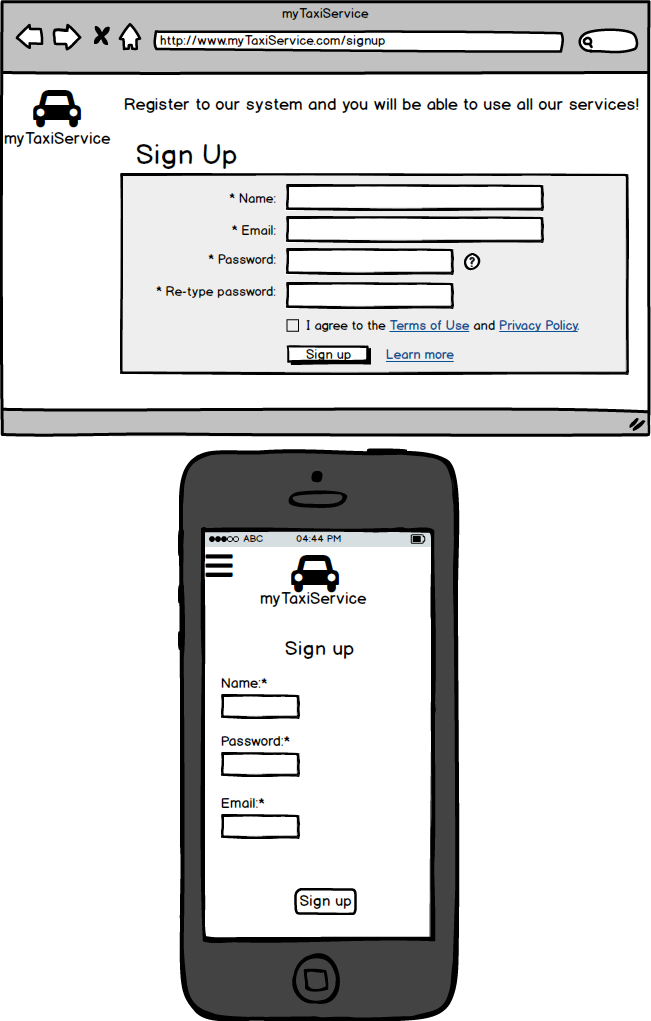
\includegraphics[width=0.9\linewidth]{Pictures/Signup}
	\end{center}
	\pagebreak
	
	\paragraph{Login} This page shows the login form for the final users.
	\begin{center}
		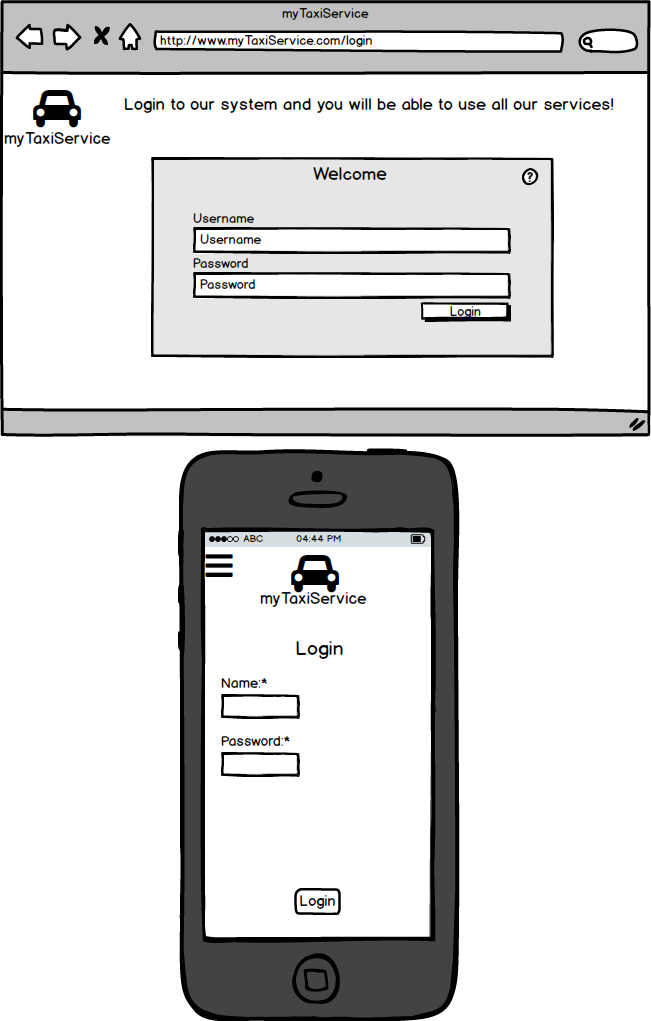
\includegraphics[width=0.9\linewidth]{Pictures/Login}
	\end{center}
	\pagebreak
	
	\pagebreak
	\paragraph{Call a taxi} The user can ask for a taxi providing the pickup location through a complete address or through the automatic detection of his/her location thanks to the browser or the GPS. The user can also choose from an history of ``recent addresses''.
	\begin{center}
		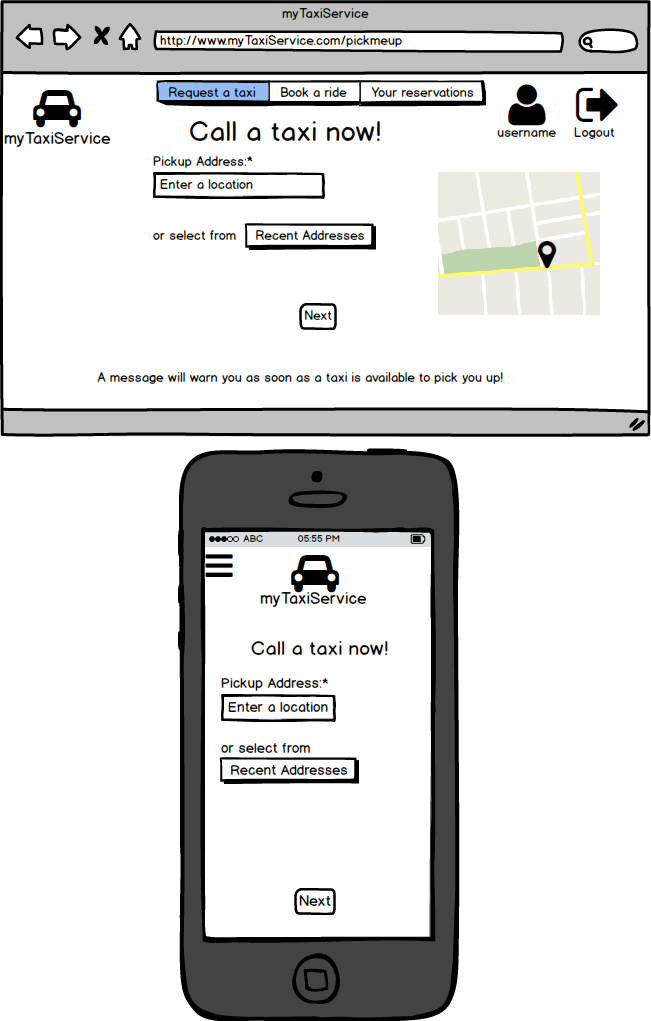
\includegraphics[width=0.9\linewidth]{Pictures/CallATaxi}
	\end{center}
	\pagebreak
	
	\paragraph{Plan a ride} The user can plan a ride in advance providing the pickup and drop off locations, the date and time, the willingness to share the ride.
	\begin{center}
		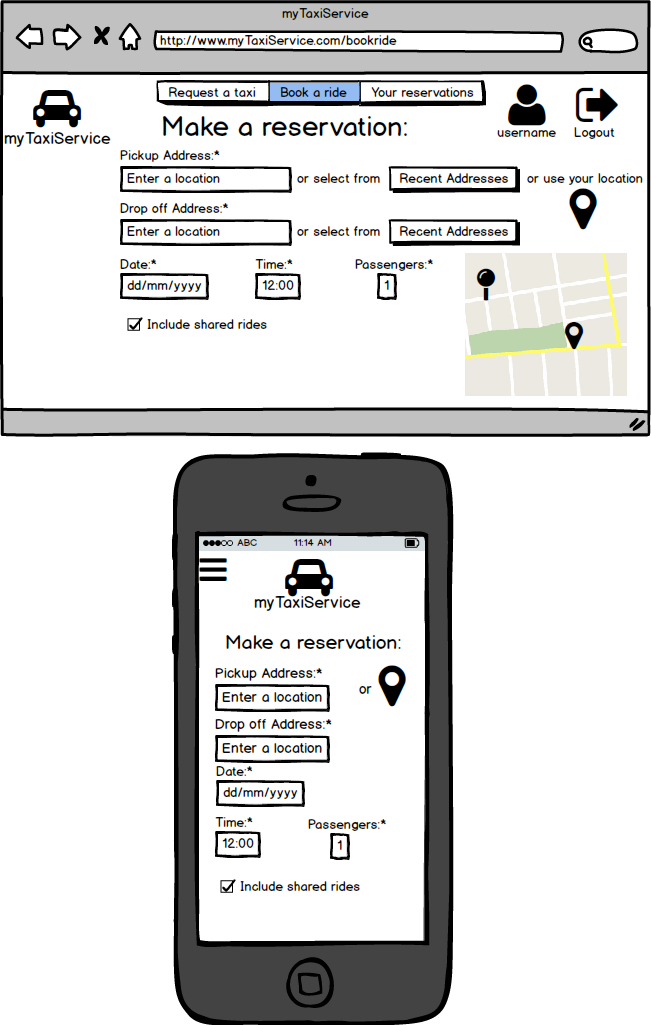
\includegraphics[width=0.9\linewidth]{Pictures/PlanAndBookARide}
	\end{center}
	\pagebreak
	
	\paragraph{Your reservations} The user can see both the active reservations and the past ones. S/he can edit the active reservations within the established time frame before the meeting time.
	\begin{center}
		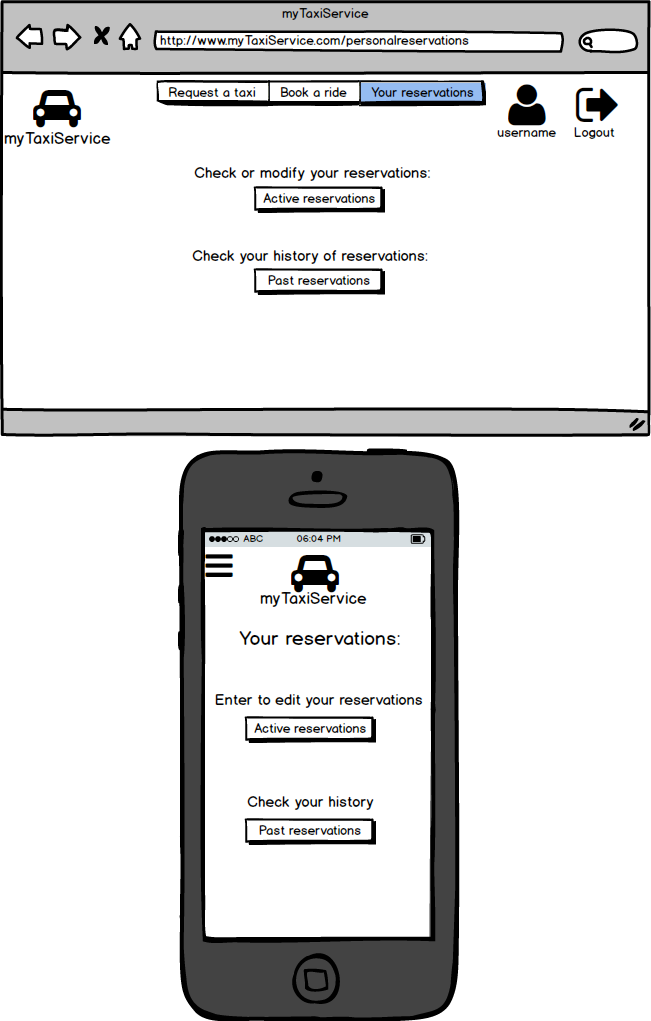
\includegraphics[width=0.9\linewidth]{Pictures/YourReservations}
	\end{center}
	\pagebreak
	
	\paragraph{Your profile} The user can edit the personal profile modifying the password, phone number, email address, permanent address, payment method.
	\begin{center}
		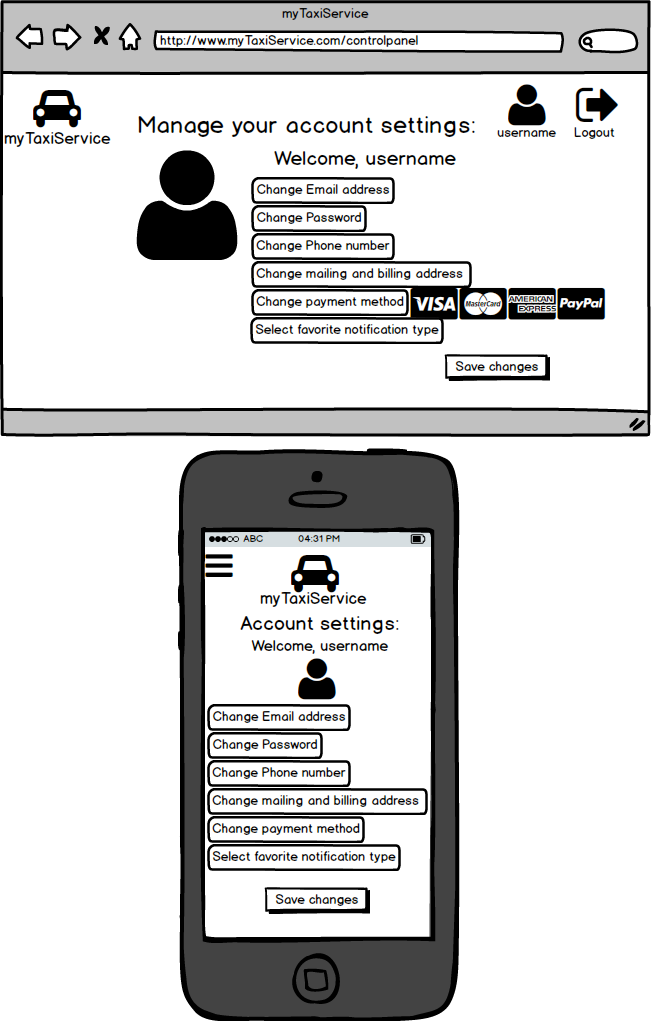
\includegraphics[width=0.9\linewidth]{Pictures/AccountPage}
	\end{center}
	\pagebreak
	
	\paragraph{Manage jobs} The taxi driver's home page: s/he can accept or reject the requests forwarded by the system and set her/his own ``availability''.
	\begin{center}
		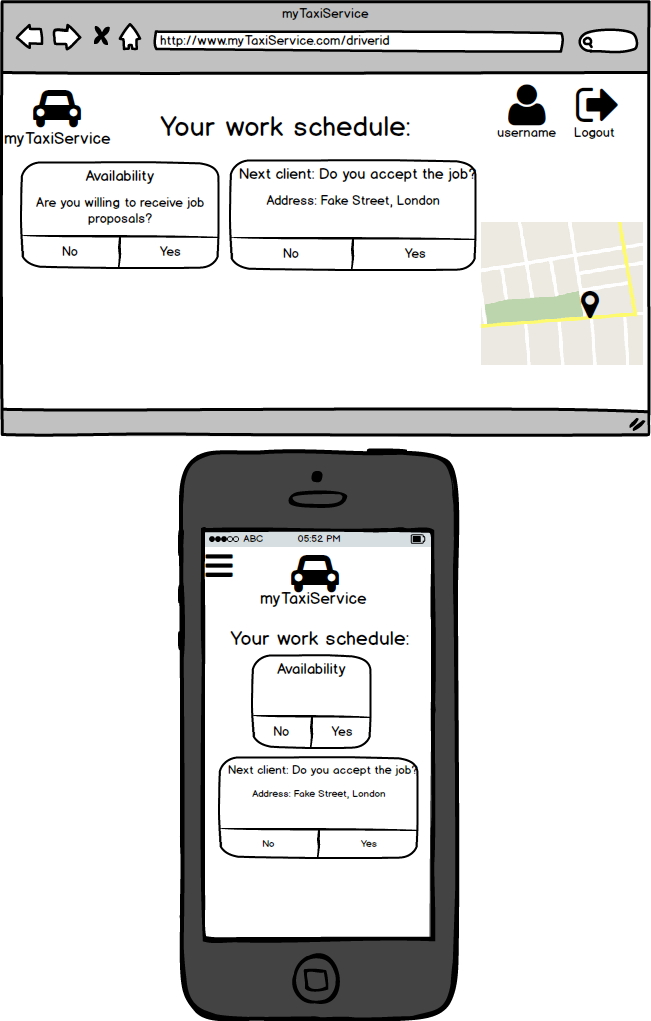
\includegraphics[width=0.4\linewidth]{Pictures/DriverPage}
	\end{center}
	\pagebreak
	
	\paragraph{Administrator panel} The administrator's home page: s/he can monitor the whole system or manage taxi drivers inserting new employees in the system DB or modifying/deleting existing ones.
	\begin{center}
		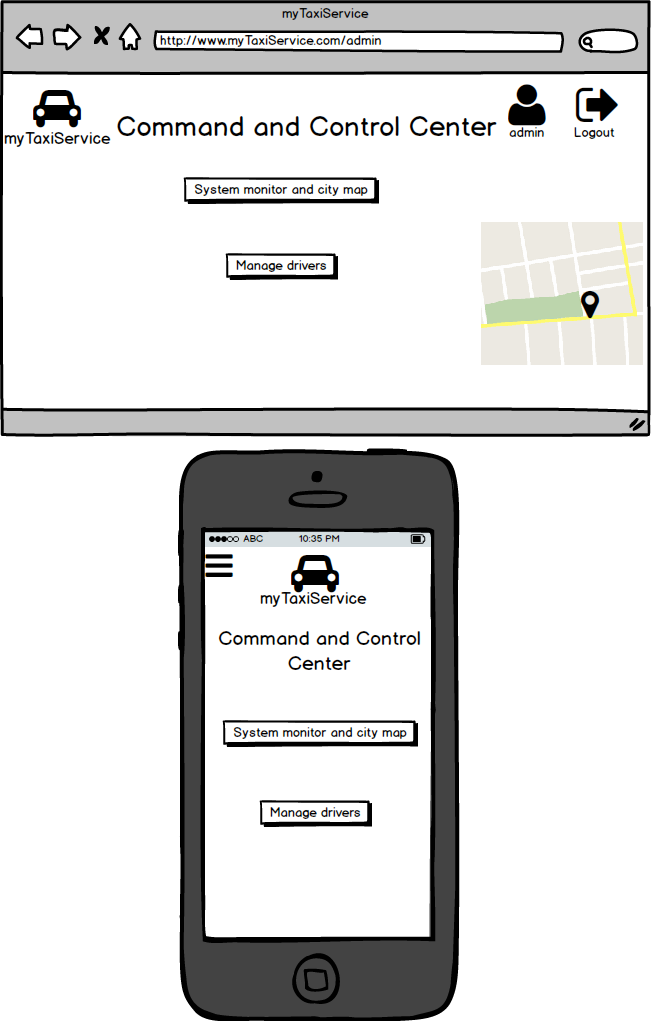
\includegraphics[width=0.9\linewidth]{Pictures/AdminPage}
	\end{center}
	\pagebreak	
	
	\subsubsection{Hardware Interfaces} \mts{} does not require and does not support any additional HW interface, it is enough a compatible smartphones or any supported browser on a computer.
	
%	\subsubsection{Software Interfaces} \textcolor{red}{do we have to pretend to use sql, java ee....???}
	
	\subsubsection{Communication Interfaces} \mts{} uses the TCP transport protocol and HTTP/HTTP over SSL application layer protocol to guarantee the top of the line security on the matter of transmission of private data.
	
	\subsection{Functional Requirements}
	
	\subsubsection{{[}G1{]} The system has to guarantee to the user the possibility to access the service either through a web application or a mobile application.}
	\begin{itemize}
		\item {[}D1{]} The system must offer the same functionalities to the final user in both cases.
	\end{itemize}
	
	\subsubsection{{[}G2{]} The system has to guarantee a fair management of the queues in each taxi zone.}
	\begin{itemize}
		\item {[}R1{]} The system is able to control the queue of taxis in every zone and enforce the predetermined priority rules to guarantee a fair management of the queues.
		\item {[}R2{]} If the taxi driver on top of the queue accepts a job then the system allocates the taxi for the specific request and therefore updates the queue.
		\item {[}R3{]} If the taxi driver on top of the queue rejects the job then the system updates the queue placing the second taxi as first and the one that rejected the job in the last position of the queue of the same zone.
		\item {[}D1{]} Each taxi queue is never empty.
	\end{itemize}
		
	\subsubsection{{[}G3{]} The system has to assign each taxi to the correct taxi zone using the GPS coordinates that receives from each taxi.}
	\begin{itemize}
		\item {[}R1{]} The system is able to map the position of the taxi fleet and assign each taxi to a predetermined zone of the city according to its position.
		\item {[}D1{]} The GPS coordinates are always available and correct.
	\end{itemize}
	
	\subsubsection{{[}G4{]} The system has to allocate a taxi for each request or reservation.}
	\begin{itemize}
		\item {[}R1{]} In case of a request the system allocates a taxi as soon as a driver in the corresponding zone accepts the job.
		\item {[}R2{]} In case of a reservation the system allocates the taxi 10 minutes before the meeting time with the client.
		\item {[}R2{]} The system computes the matching of people in shared rides taking into account the number of passengers from each reservation; the total number of passengers cannot exceed the capacity of the taxi.
		\item {[}D1{]} There is always at least one available taxi.
	\end{itemize}
		
	\subsubsection{{[}G5{]} The system has to notify the users, both passengers and taxi drivers, about updates on taxi requests and reservations in which they are involved.}
	\begin{itemize}
		\item {[}R1{]} The awaiting passenger is notified by the system if the taxi is delayed for any reason.
		\item {[}R2{]} The passenger is notified when other passengers sharing the same route join the ride or cancel the reservation; the user is also updated with the recomputed taxi fare.
		\item {[}R3{]} The system notifies the taxi driver allocated to a request if the correspondent passenger has deleted the reservation.
		\item {[}R4{]} The system allows passengers to choose the type of notification they will receive among text message, email and mobile push notification.
		\item {[}D1{]} The taxi driver will always receive only mobile push notifications.
		\item {[}D2{]} The user will provide his preference on at least one type of notification.
	\end{itemize}
		
	\subsubsection{{[}G6{]} The system has to offer public APIs to enable the possibility to develop additional services on top of the basic ones.}
	\begin{itemize}
		\item {[}R1{]} The system offers APIs to third party applications using web APIs as technology.
		\item {[}R2{]} The system replies using current industry standards.
		\item {[}D1{]} Access to APIs functionalities is provided only using the HTTPS protocol.
	\end{itemize}
		
	\subsubsection{{[}G7{]} The passenger shall be able to sign up to the service.}
	\begin{itemize}
		\item {[}R1{]} The user cannot register more than once.
		\item {[}R2{]} The user must choose a username not already used by someone else.
		\item {[}R3{]} Unregistered users can only see the sign up and login page.
		\item {[}R4{]} The user must fill in all the mandatory fields of the proposed form to successfully complete the registration process.
		\item {[}D1{]} Phone number, email address and credit card data used for the registration are mandatory and must be valid.
	\end{itemize}
		
	\subsubsection{{[}G8{]} The passenger shall be able to log in to the service.}
	\begin{itemize}
		\item {[}R1{]} If the user hasn't the correct login information cannot access the system.
		\item {[}R2{]} If the user provides correct credentials the system will grant him/her the access.
		\item {[}D1{]} The system does not implement a password retrieval mechanism.
	\end{itemize}
		
	\subsubsection{{[}G9{]} The passenger shall be able to request a taxi.}
	\begin{itemize}
		\item {[}R1{]} The user can ask for a taxi simply providing his/her own position.
		\item {[}R2{]} The system is able to dispatch the request of the client to the right queue according to his/her position.
		\item {[}R3{]} The system has to answer a taxi request by informing the passenger about the code of the taxi and the waiting time.
		\item {[}R4{]} When a passenger books a ride s/he is given a code that uniquely identifies her/him in front of the taxi driver.
		\item {[}D1{]} The user knows that the capacity of the taxi is 4 passengers.
		\item {[}D1{]} If there are more than 4 passengers the user has to make two or more requests.
	\end{itemize}
	
	\subsubsection{{[}G10{]} The passenger shall be able to delete a taxi request.}
	\begin{itemize}
		\item {[}R1{]} The passenger can withdraw the request within 30 seconds after the call.
		\item {[}R2{]} A penalty fee is automatically collected if the user deletes the request after the allowed time frame.
		\item {[}D1{]} Passengers always wait for the requested taxi.
	\end{itemize}
	
	\subsubsection{{[}G11{]} The passenger shall be able to create a reservation for a taxi ride.}
	\begin{itemize}
		\item {[}R1{]} The user can customize the reservation, specifying the date and time of the ride, the origin and destination and the number of passengers.
	\end{itemize}
	
	\subsubsection{{[}G12{]} The passenger shall be able to modify or delete a taxi reservation.}
	\begin{itemize}
		\item {[}R1{]} The user can check his/her own reservations and edit or delete them.
		\item {[}D1{]} If the user deletes a reservation in the last 10 minutes before the meeting time (the taxi has already been allocated), then there is a fixed penalty fee automatically deducted from the user's credit card.
	\end{itemize}
	
	\subsubsection{{[}G13{]} The passenger shall be able to enable taxi sharing option.}
	\begin{itemize}
		\item {[}R1{]} The user can enable the sharing of a reservation.
		\item {[}D1{]} This is only valid for reservations booked in advance.
	\end{itemize}
	
	\subsubsection{{[}G14{]} The passenger shall be able to join a shared reservation.}
	\begin{itemize}
		\item {[}R1{]} The system computes the matching of people in shared rides taking into account the number of passengers from each reservation; the total number of passengers cannot exceed the capacity of the taxi.
		\item {[}D1{]} This is only valid for reservations booked in advance.
		\item {[}D2{]} Passengers sharing a ride will be matched only if they share the same pick up and destination zone.
	\end{itemize}
	
	\subsubsection{{[}G15{]} The passenger shall be able to see historical data on his taxi rides.}
	\begin{itemize}
		\item {[}R1{]} The system keeps track of the recent routes and addresses.
		\item {[}R2{]} The user can select locations from past rides to plan new ones.
	\end{itemize}

	\subsubsection{{[}G16{]} Taxi drivers shall be able to log in to the service.}
	\begin{itemize}
		\item {[}R1{]} If the user hasn't the correct login information cannot access the system.
		\item {[}R2{]} If the user provides correct credentials the system will grant him/her the access.
		\item {[}D1{]} The system does not implement a password retrieval mechanism.
		\item {[}D2{]} Only legally employed taxi drivers have the login information to access the system.
	\end{itemize}
	
	\subsubsection{{[}G17{]} Taxi drivers must inform the system about their availability.}
	\begin{itemize}
		\item {[}R1{]} The system allows taxi drivers to set their availability.
		\item {[}R2{]} The system allows to specify the reason of the unavailability.
		\item {[}D1{]} All the actions performed by a taxi driver during working hours will be performed through the mobile application.
		\item {[}D2{]} Taxi drivers always remember to switch their availability.
	\end{itemize}
	
	\subsubsection{{[}G18{]} Taxi drivers must confirm if they are going to take care of a certain call.}
	\begin{itemize}
		\item {[}R1{]} The system allows taxi drivers to accept or reject a call.
		\item {[}D1{]} Taxi drivers always remember to accept or reject a call.
	\end{itemize}	
					
	\subsubsection{{[}G19{]} The administrator shall be able to add, edit and delete taxi drivers in the system.}
	\begin{itemize}
		\item {[}R1{]} The system allows to the administrator to add, edit and delete taxis.
		\item {[}D1{]} The administrator only inserts in the system already verified entitled taxi drivers.
	\end{itemize}	
	
	\subsubsection{{[}G20{]} The administrator shall be able to manage and supervise the operation of the whole system, including the real-time situation of all the queues and of the taxis.}
	\begin{itemize}
		\item {[}R1{]} The system allows to the administrator to have a glance view of the system situation.
		\item {[}D1{]} The visualization is read only.
	\end{itemize}							
		
	\subsection{The world and the machine} ``The World \& The Machine''	model by M. Jackson \& P. Zave has been used as an additional domain analysis of \mts{} application. This approach identifies the portion of ``The World'' affected by ``The Machine'', the portion of system to be developed, and the intersection (``Shared Phenomena'') between the world and the application, that are all world information known or
	managed directly by the application.\\\textcolor{red}{INSERT SCHEMA HERE}
	
	\subsection{Scenarios}
	
	\subsubsection{Scenario 1} Bob lives in Milan, a very crowded and traffic congested city, for this reason he decided not to buy a car. When he needs to move around the city he finds very convenient the taxi service, less crowded than other public transport means. By now he has learned how to use all the different functionalities offered by \mts{} mobile application. Whenever and wherever he needs he simply start the application on his mobile phone and he requests a taxi in a matter of seconds simply providing his location through the built-in GPS of his smartphone. In a very short time, usually no more than a couple of minutes, he receives the notification that confirms the take on responsibility of his call with the code of the incoming taxi and the estimated waiting time. Meanwhile the system reserves on the credit card he linked the minimum fee in case of cancellation. Once the taxi arrives Bob exhibits the identification code to the taxi driver and is taken to his destination; finally the system automatically computes the fare based on the distance covered and deducts the correct amount of money from his credit card. 
	
	\subsubsection{Scenario 2} Alice has just moved to Milan and hasn’t got any car. For this reason, she looks on the Internet to understand which options she has to move around the city with public transports and she finds {\em myTaxyService}'s website that presents the taxi service. She decides to sign up to make use of the service, so she provides her personal data including the data of her credit card and selects ``email'' as notification option. Once the 2-step verification process is successfully completed she logins with the credentials chosen during the registration process. She is now operative and wants to try out the service, so she enters the booking page to make a reservation for the next day. She fills in the pickup address with her own and the destination field with the museum she wants to visit and sets the date and time, enabling the shared ride choice and finally submits the request. The system confirms the reservation process went through. 
	
	\subsubsection{Scenario 3} Alice is invited to her friend’s Bob birthday party held the next evening at Bob’s house, so she logins to the {\em myTaxyService}'s website to reserve a taxi for tomorrow night. Unfortunately, she doesn’t recall her friend’s address, but she remembers that the previous week they took a taxi together to his house, so she browses the history of her own reservation and from there recognizes Bob’s house address, then Alice uses it as drop off location and completes the reservation. Unluckily the following morning Bob phones to Alice and warns her that the party is postponed indefinitely due to bad weather forecast. Alice then decides to delete the reservation for taxi for the night, so she logins to the website and cancel the booking without paying any fees.
	
	\subsubsection{Scenario 4} Mike is a taxi driver in Milan and its company relies on \mts{} for the management of the work. He received the access codes to the system once he had been employed. Now every morning he starts his daily work routine by starting the \mts{} app on his phone and heading to the assigned zone with his taxi to pick up the first client. He switches on the ``availability’’ to work and starts receiving job proposals. Mike accepts them almost always; he only takes the liberty to switch off the system for a 30-minute lunch break. Often it happens that he has to pick up two clients in the same area for a shared ride because they are headed in the same direction. The shared ride feature has been having an huge approval among the clients since the implementation of the \mts{} application. At the end of the day Mike stops the flow of job proposals setting the ``availability’’ back again to off and returns to his family at home.
	
	\subsubsection{Scenario 5} Jack is the manager of the taxi company in Milan and therefore he is the administrator of the \mts{} system. He spends his days monitoring the activity of the system thanks to the supervision functionality of the system. He can access it anytime anywhere thanks to the double interface for web browser and mobile application. Of course he prefers the bigger monitor of his computer when he’s in the office with respect to the small display of the smartphone, but he is more relaxed knowing that he is notified if something goes wrong even when he is outside the office. Often it happens that he needs to insert in the system new just employed drivers; in that case he collects all the information about the person and register the user with the specific functionalities for the drivers.
	
	\pagebreak
	
	\subsection{UML Models}
	
	\subsubsection{Use Case}
	
%	\AddToShipoutPictureBG*{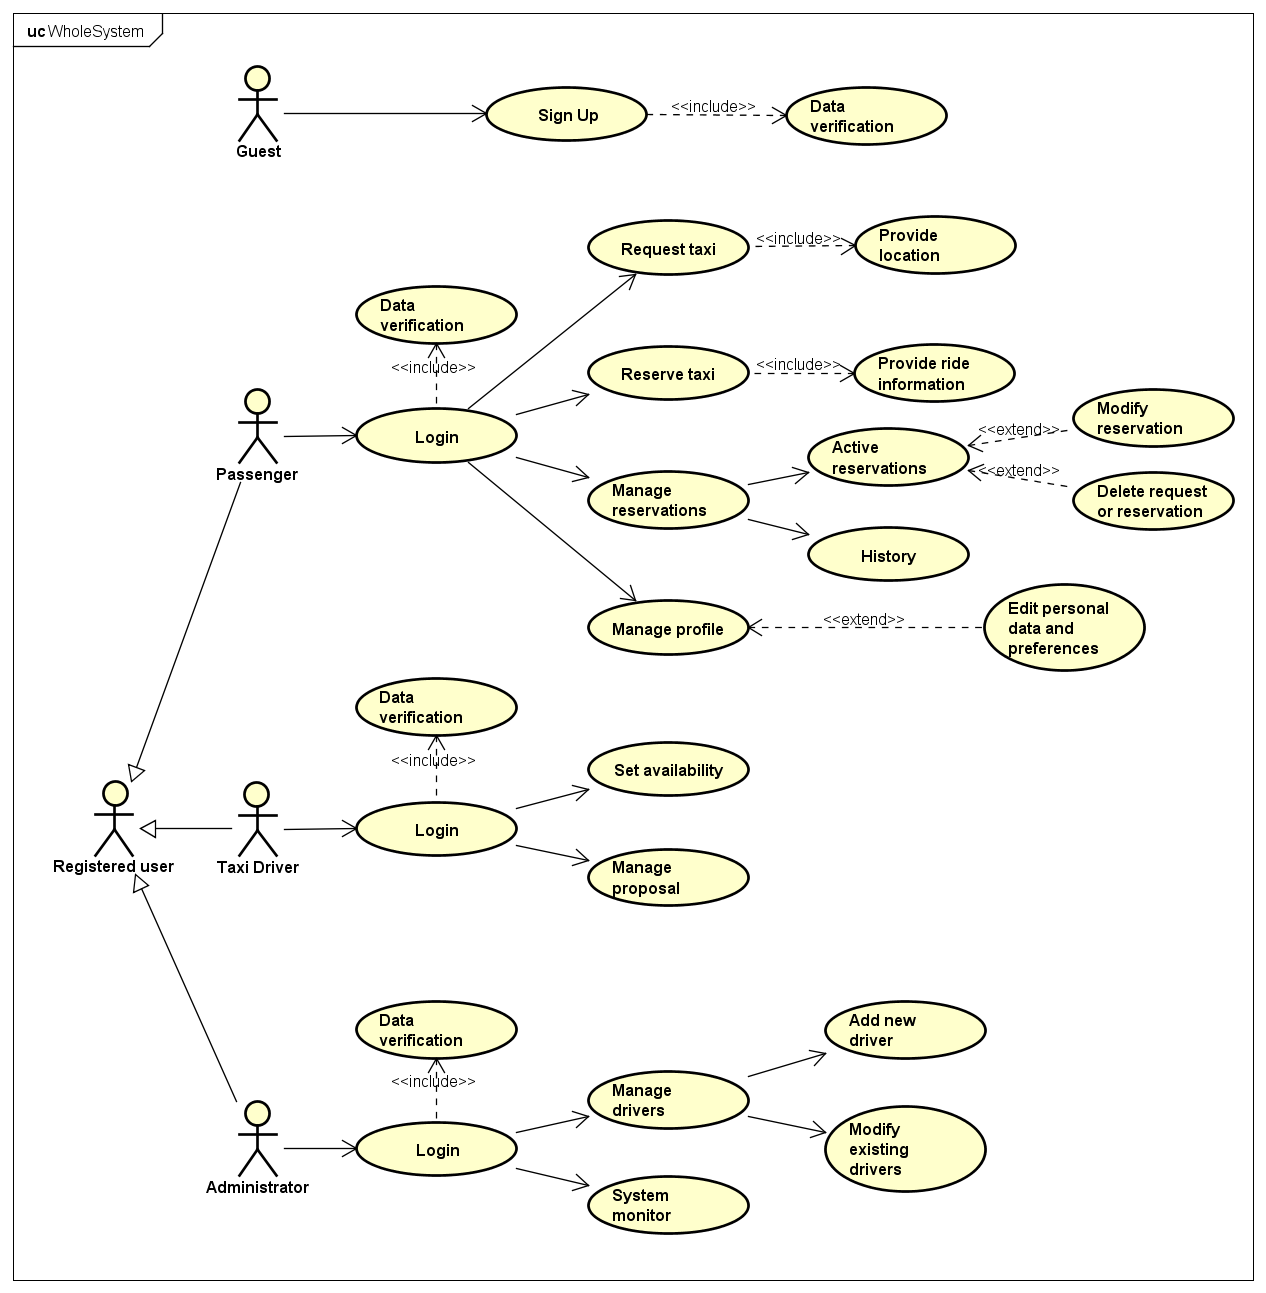
\includegraphics[width=\paperwidth,height=\paperheight]{Pictures/UCWholeSystem}}
%	\begin{figure}[h]
%		\centering
%	%	\begin{center}
%			%			\centerline{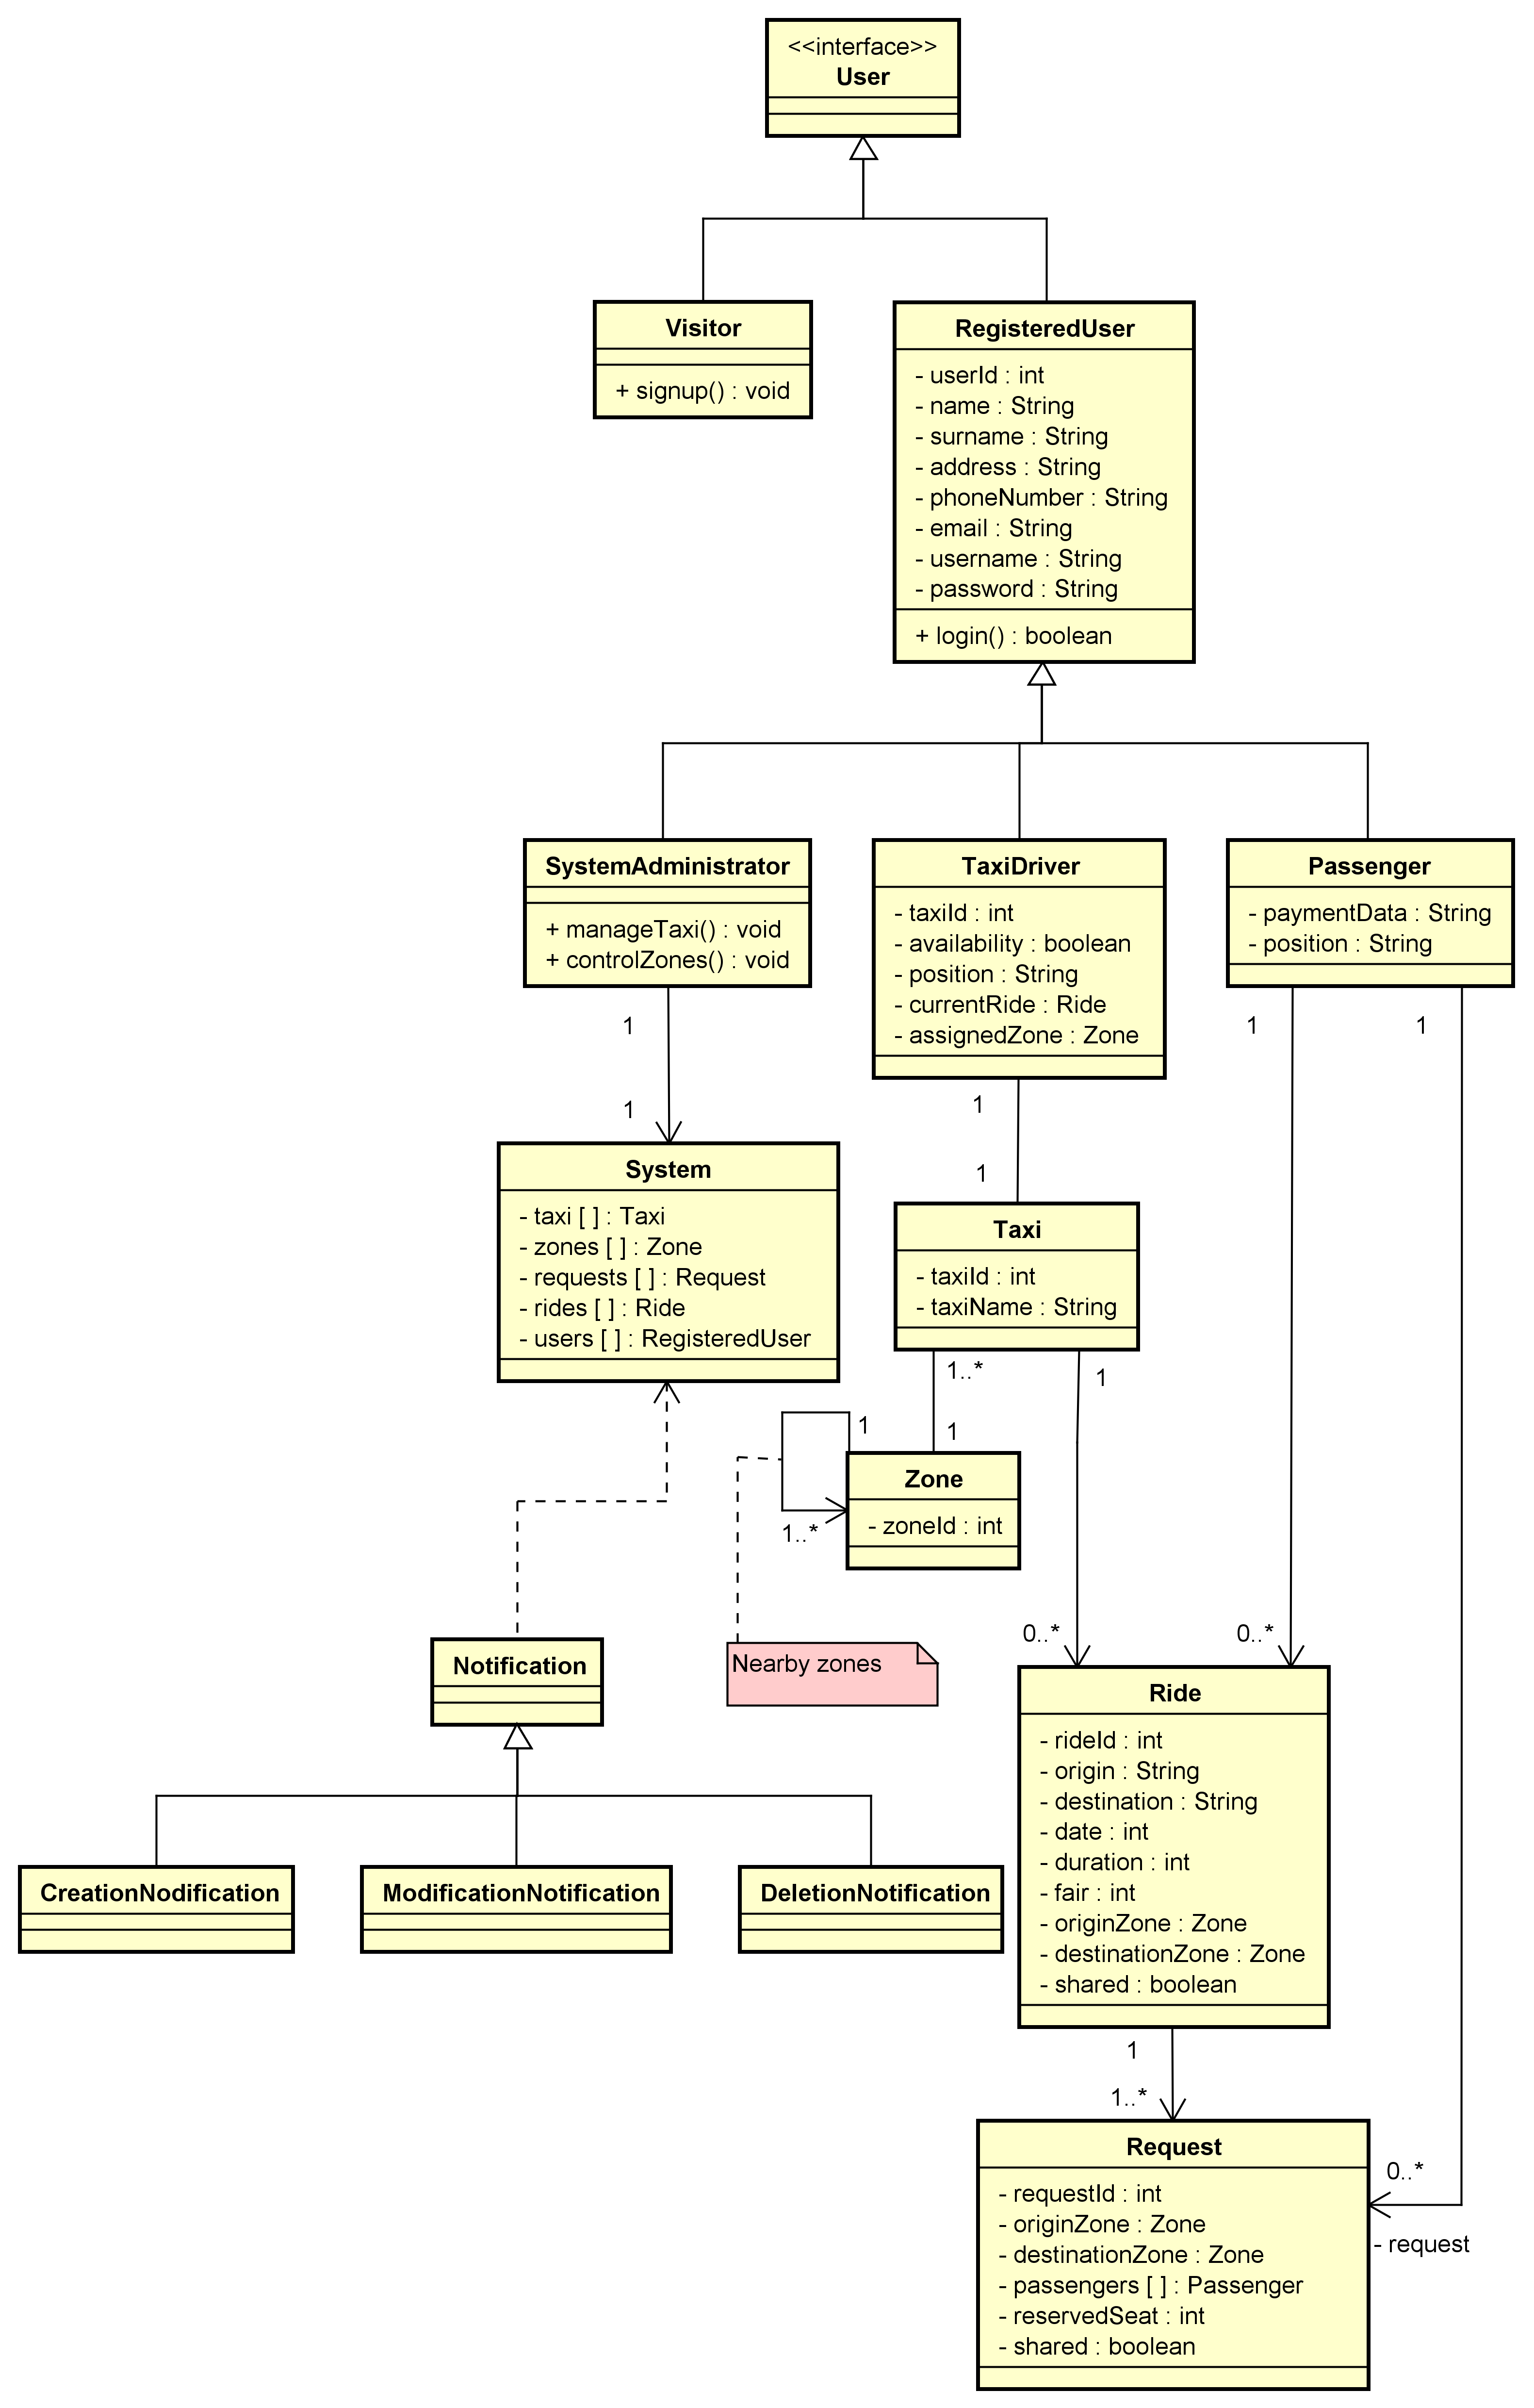
\includegraphics[width=1.4\linewidth]{Pictures/ClassDiagram}}
%%			\vspace*{-2.5cm}
%			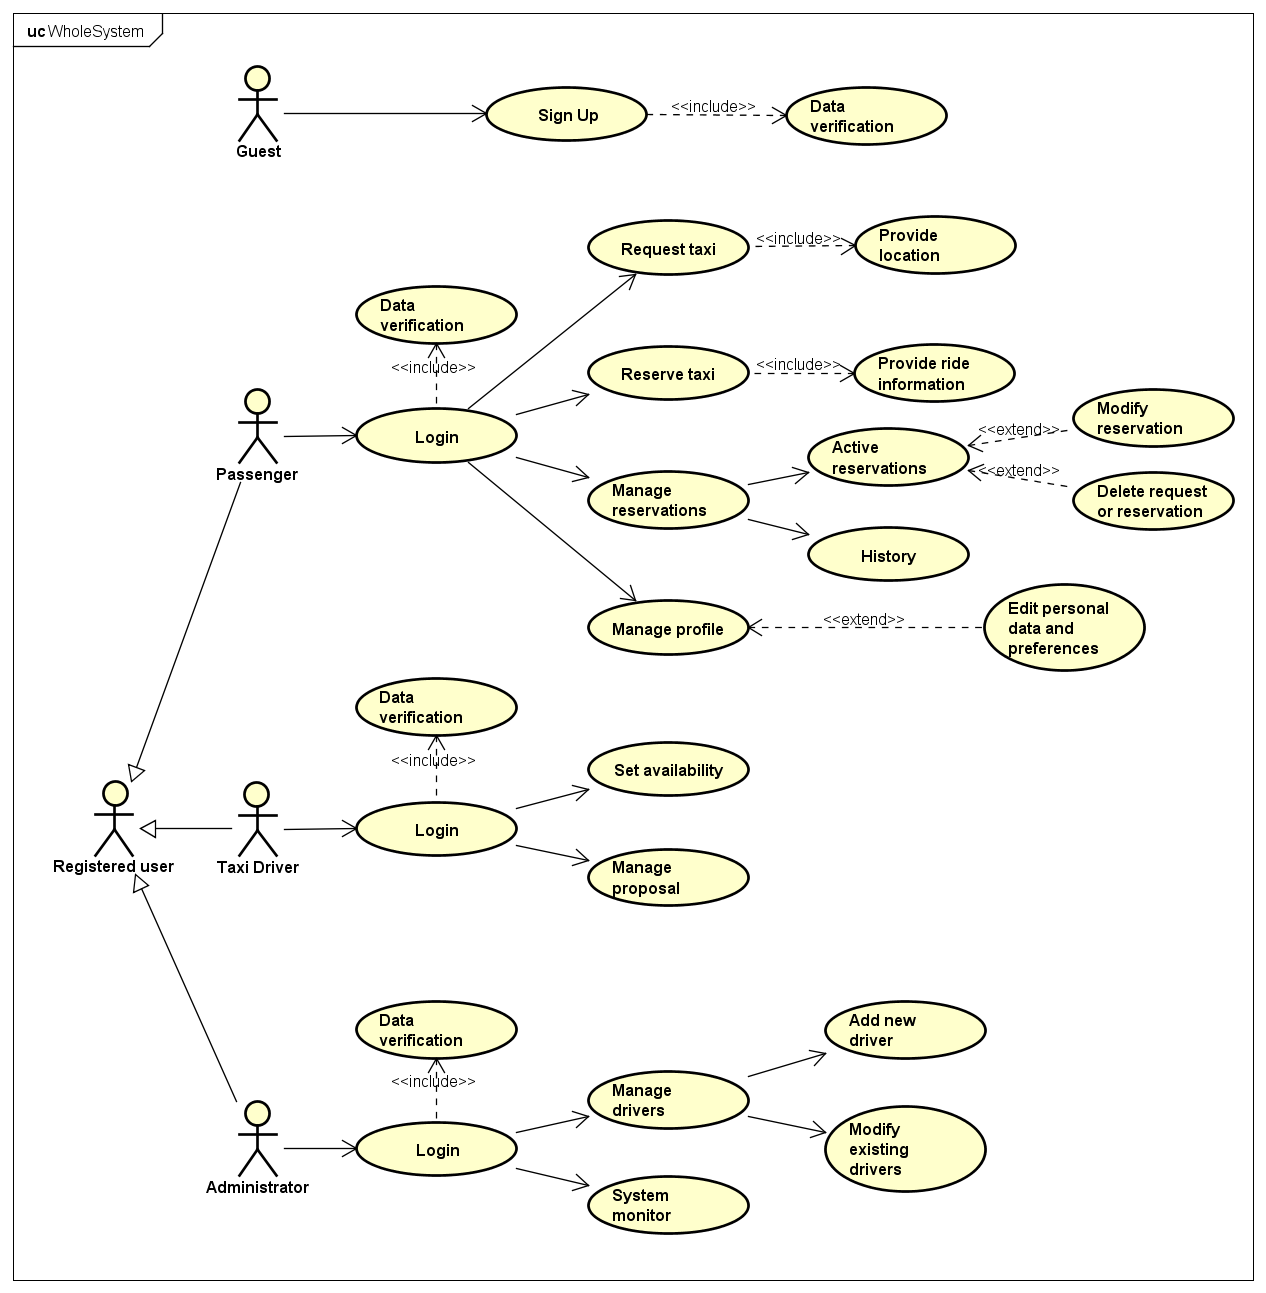
\includegraphics[width=0.95\linewidth]{Pictures/UCWholeSystem}
%					
%	%	\end{center}
%	\end{figure}

	\noindent%
	\begin{minipage}{\linewidth}% to keep image and caption on one page
		\makebox[\linewidth]{%        to center the image
		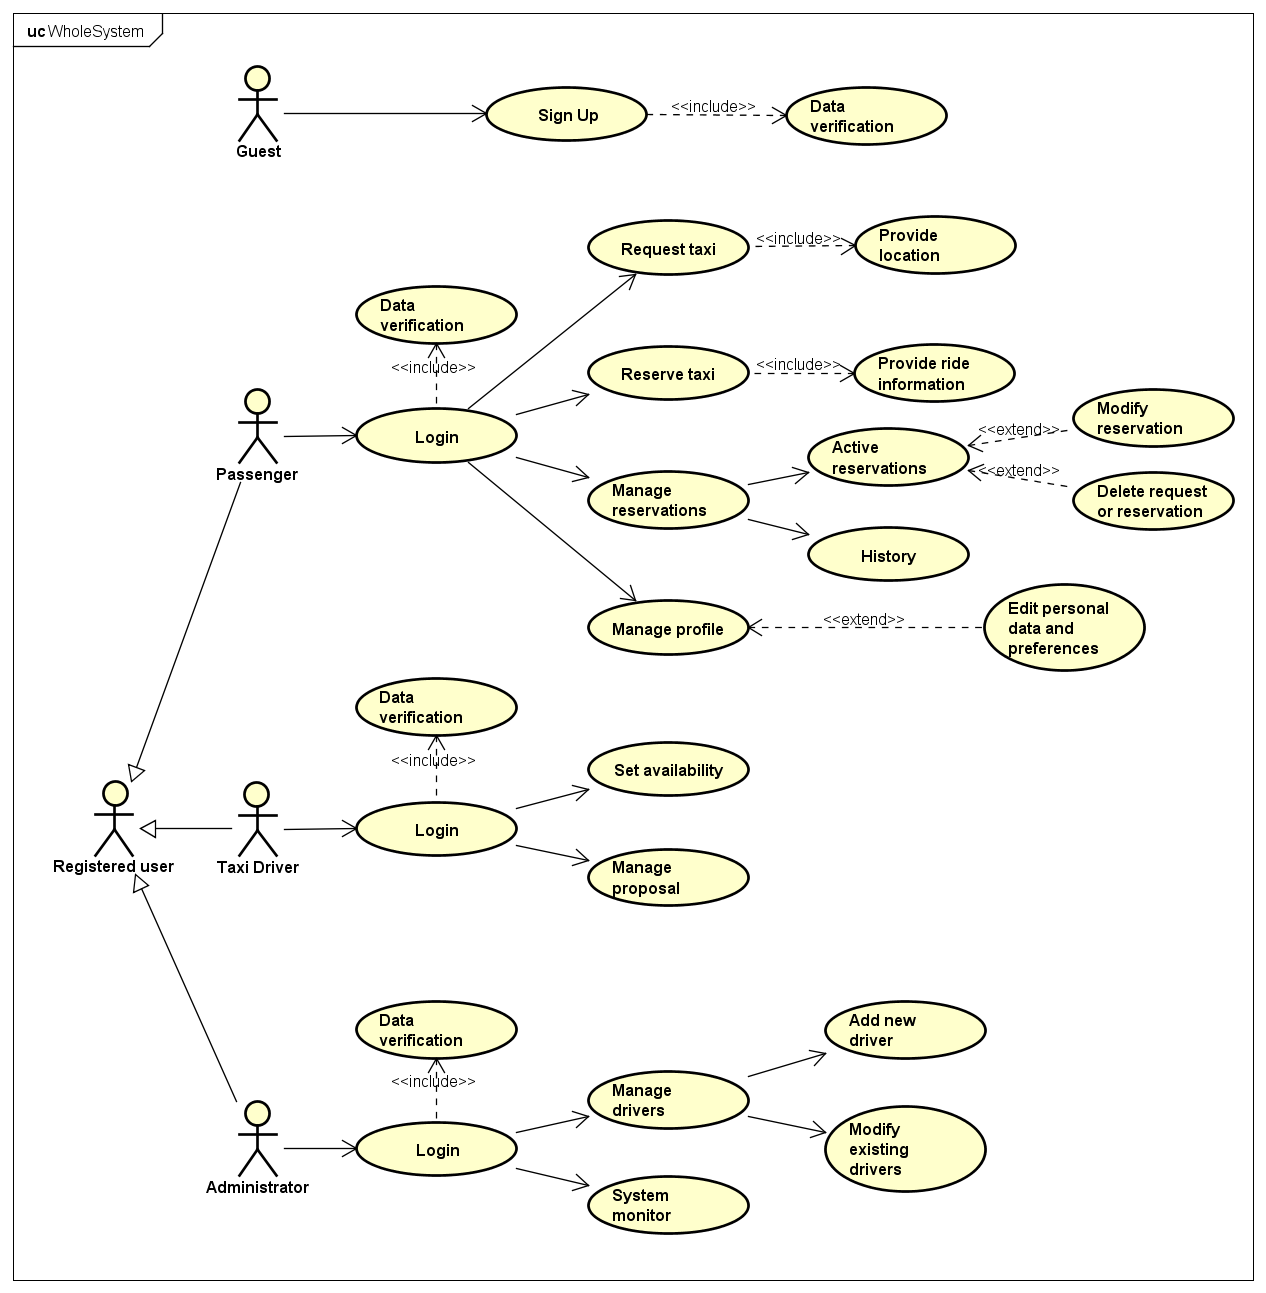
\includegraphics[keepaspectratio=true,scale=0.62]{Pictures/UCWholeSystem}}
	\end{minipage}
	
	\pagebreak
	
	\renewcommand{\arraystretch}{1.5}
	\setlength{\tabcolsep}{6pt}
	\paragraph{Guest registers to \mts{}}
	
	\begin{center}
		\begin{tabular}{| l | p{9cm} |}\hline
			Actor & Guest\\\hline
			Goal & {[}G7{]} \\\hline
			Input Condition & NULL\\\hline
			Event Flow & \begin{enumerate}
							\item Guest on the home page clicks on ``Sign up''.
							\item Guest fills in at least all mandatory fields.
							\item Guest clicks on the ``confirm'' button.
							\item The application saves the data in the DB.
						 \end{enumerate}\\\hline
			Output Condition & Guest successfully completes the registration process and
								becomes a registered user. From now on s/he can login to
								the application using her/his credentials and use \mts{}.\\\hline
			Exceptions & {\begin{enumerate}
							\item The guest is already a registered user.
							\item One or more mandatory fields are not valid or missing.
							\item The username chosen is already used by another user.
							\item The email chosen is already associated to another user.
						  \end{enumerate} All exceptions are handled alerting the guest of the
						problem through an error message.}\\\hline
		\end{tabular}
	\end{center}
%	\begin{center}
%		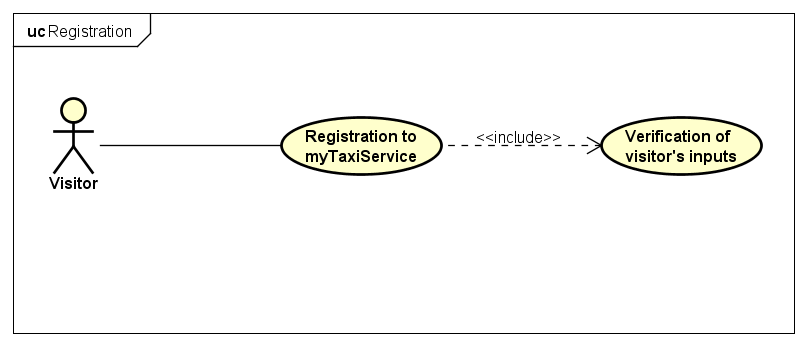
\includegraphics[width=0.9\linewidth]{Pictures/UCRegistration}
%		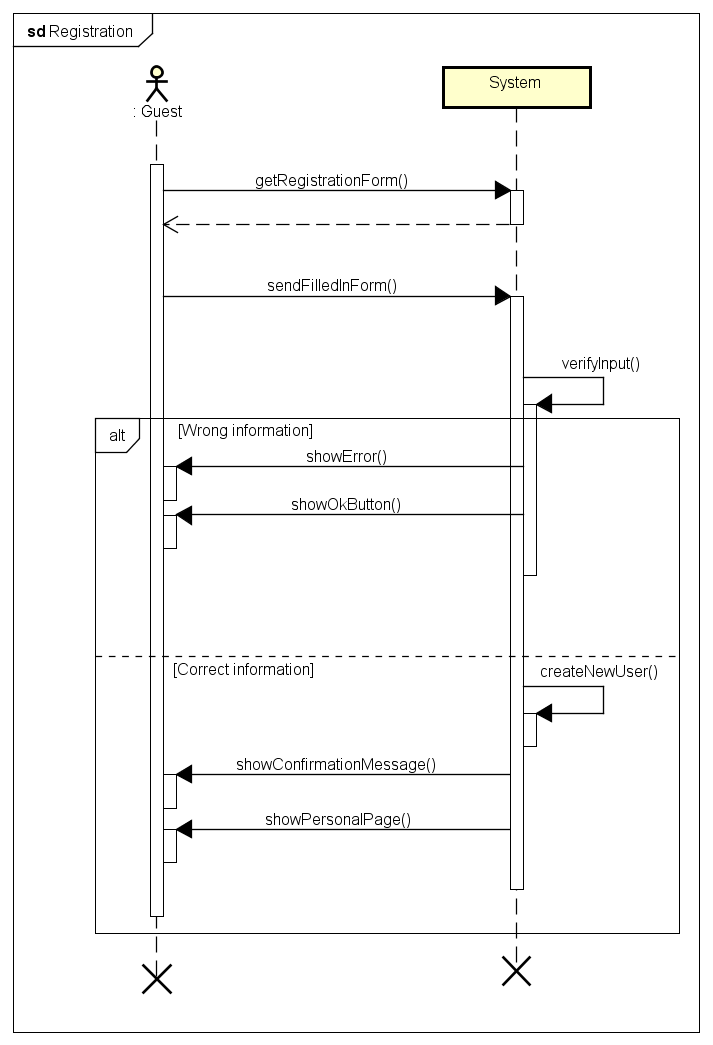
\includegraphics[width=0.9\linewidth]{Pictures/SDRegistration}
%	\end{center}

%		\newgeometry{left=1cm,bottom=1cm,right=1cm,top=1cm}

%	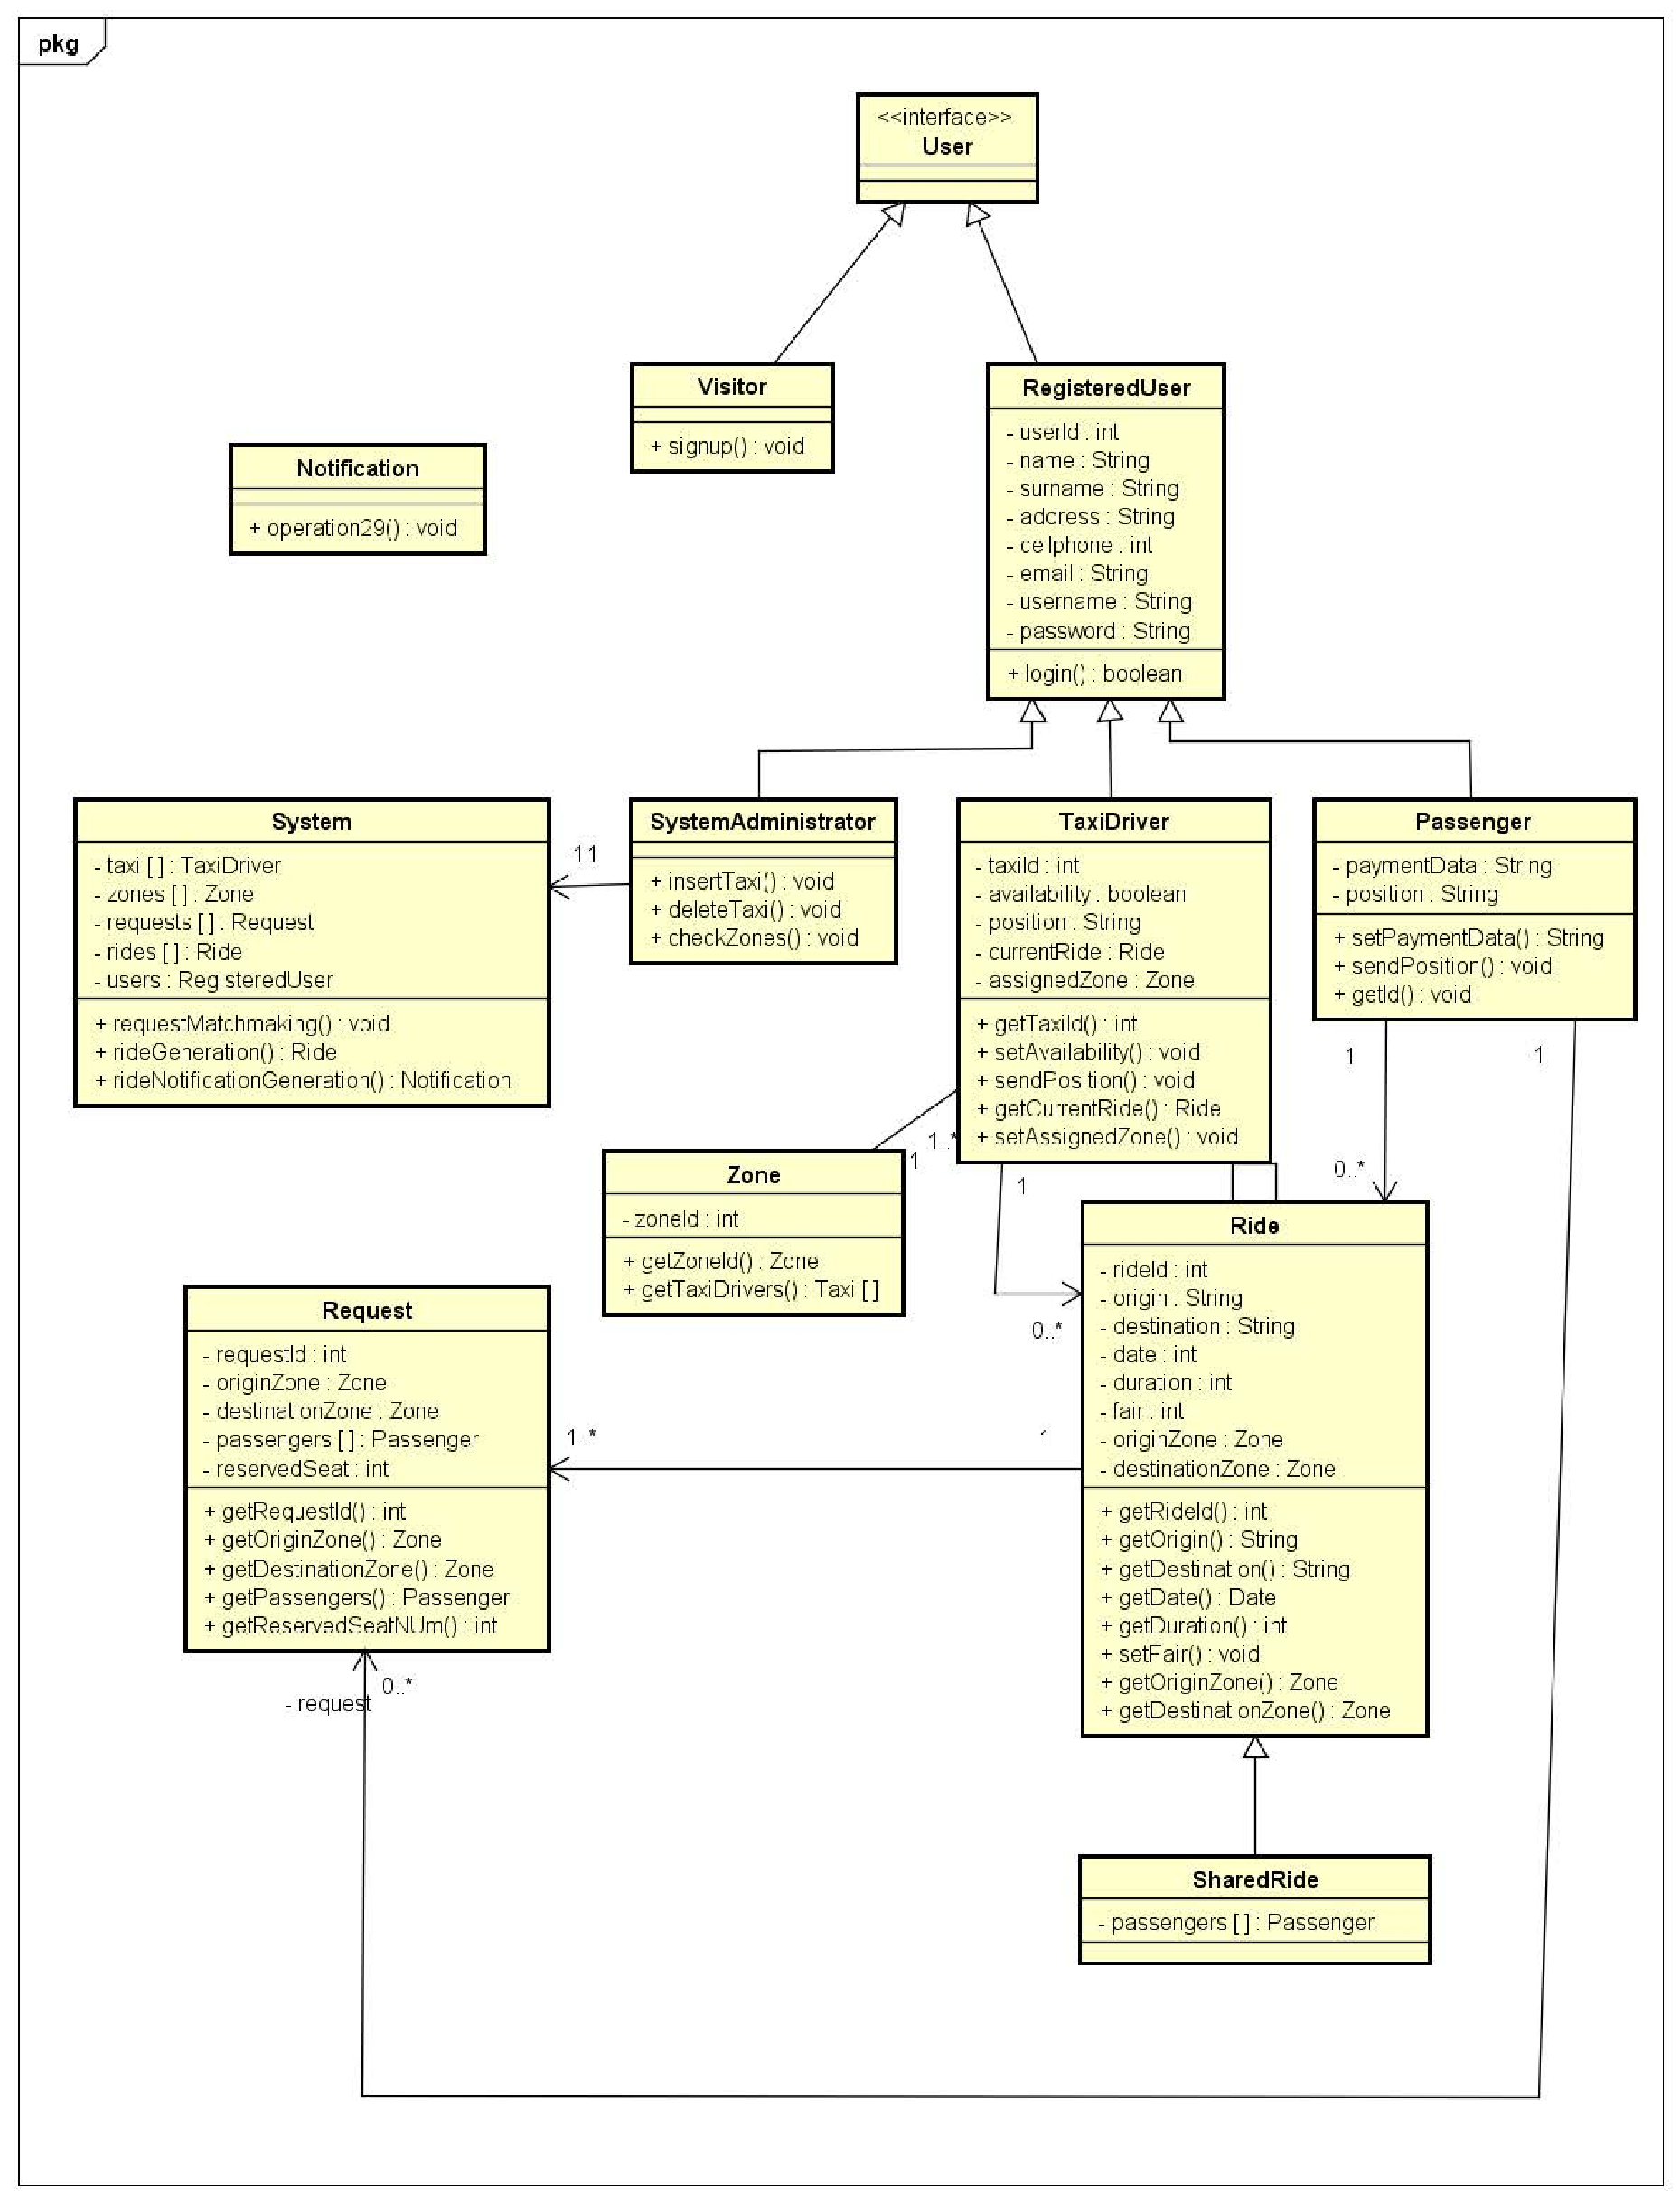
\includepdf{Pictures/ClassDiagram.pdf}
	\pagebreak
	\afterpage{}

%	\begin{figure}[p]
%		\begin{center}
%			\vspace*{-2.5cm}
%			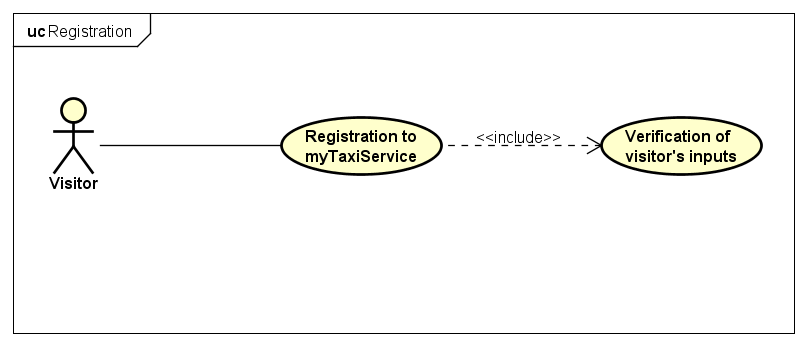
\includegraphics[width=0.95\linewidth]{Pictures/UCRegistration}
%			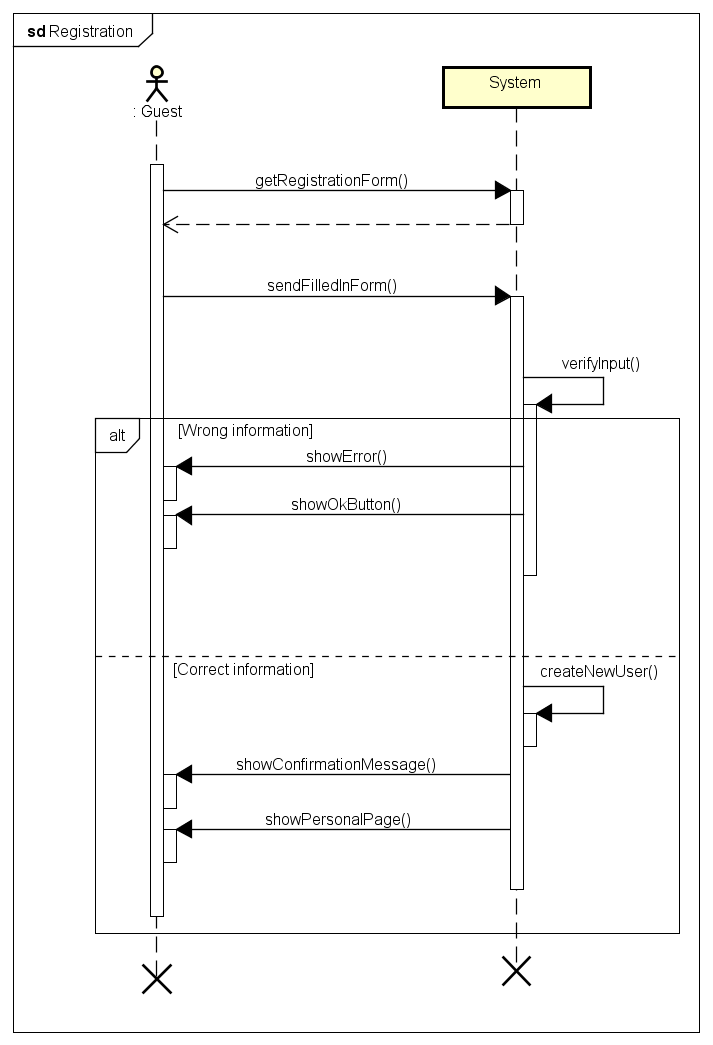
\includegraphics[width=0.95\linewidth]{Pictures/SDRegistration}
%		\end{center}
%	\end{figure}
	
		\noindent%
		\begin{minipage}{\linewidth}
			\vspace*{-0.7cm}
			\makebox[\linewidth]{
				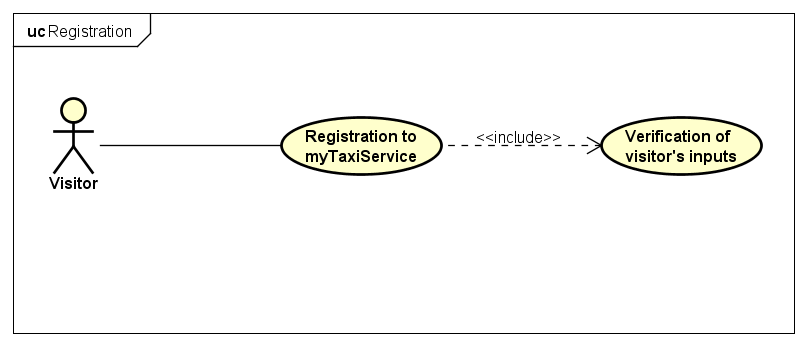
\includegraphics[keepaspectratio=true,scale=0.65]{Pictures/UCRegistration}}
		\end{minipage}
		
		\vspace*{0.5cm}
		
		\noindent%
		\begin{minipage}{\linewidth}
			\vspace*{-0.7cm}
			\makebox[\linewidth]{
				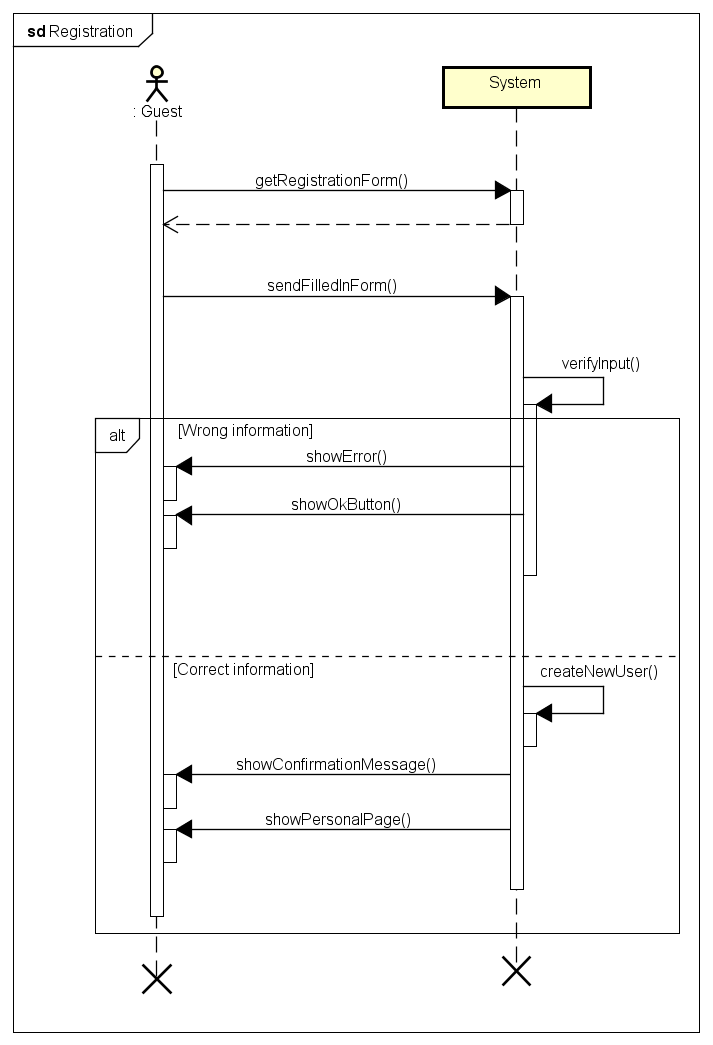
\includegraphics[keepaspectratio=true,scale=0.73]{Pictures/SDRegistration}}
		\end{minipage}
		
		
		
		


	\pagebreak	

	
	\paragraph{Guest logins to \mts{}}
	\begin{center}
		\begin{tabular}{| l | p{9cm} |}\hline
			Actor & Guest, Passenger\\\hline
			Goal & {[}G8{]} \\\hline
			Input Condition & The user must be already registered.\\\hline
			Event Flow & \begin{enumerate}
							\item \mts{} shows the login page.
							\item Guest completes the form inserting correct username and password.
						 \end{enumerate}\\\hline
			Output Condition & \begin{enumerate}
									\item \mts{} verifies the credentials of the guest and if correct shows the home page for the registered user.
									\item Guest is promoted to registered user.
							   \end{enumerate}\\\hline
			Exceptions & If username and/or password are incorrect the system notifies this to the guest through an error message.\\\hline
		\end{tabular}
	\end{center}
	
	\pagebreak
	\noindent%
	\begin{minipage}{\linewidth}
		\vspace*{-0.7cm}
		\makebox[\linewidth]{
			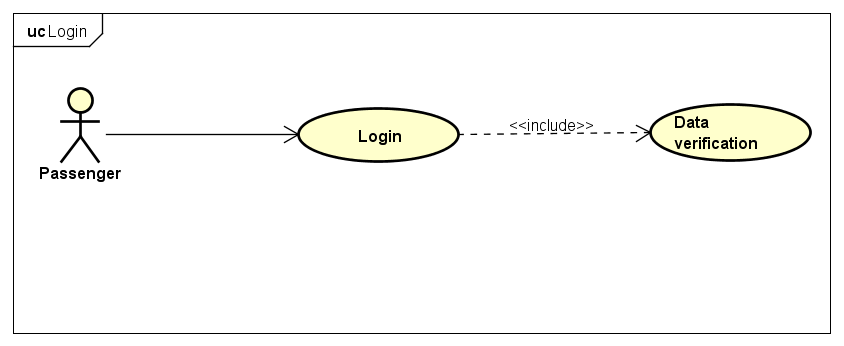
\includegraphics[keepaspectratio=true,scale=0.62]{Pictures/UCLogin}}
	\end{minipage}
		
	\vspace*{0.6cm}
		
	\noindent%
	\begin{minipage}{\linewidth}
		\vspace*{-0.75cm}
		\makebox[\linewidth]{
		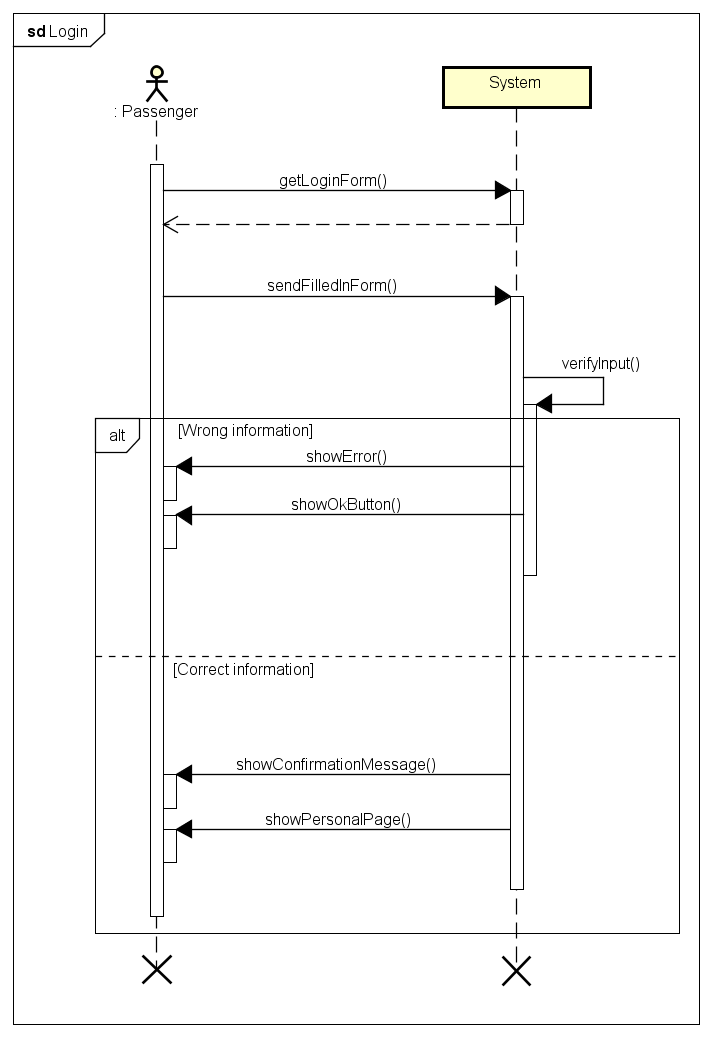
\includegraphics[keepaspectratio=true,scale=0.74]{Pictures/SDLogin}}
	\end{minipage}
		
	\pagebreak
	
	\paragraph{Passenger requests a taxi}
	\begin{center}
		\begin{tabular}{| l | p{9cm} |}\hline
			Actor & Passenger\\\hline
			Goal & {[}G9{]} \\\hline
			Input Condition & The user must be already logged in.\\\hline
			Event Flow & The user requests a taxi using any of the options to provide his/her own location.\\\hline
			Output Condition & \begin{enumerate}
									\item \mts{} starts the process in order to find a taxi for the user.
									\item Once the system has allocated a taxi it notifies the user.
							   \end{enumerate}\\\hline
			Exceptions & NULL\\\hline
		\end{tabular}
	\end{center}	
	
		\pagebreak
		\noindent%
		\begin{minipage}{\linewidth}
			\vspace*{0.5cm}
			\makebox[\linewidth]{
				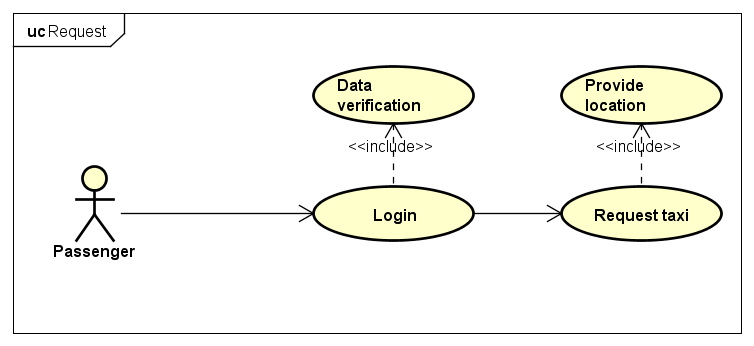
\includegraphics[keepaspectratio=true,scale=0.8]{Pictures/UCRequest}}
		\end{minipage}
		
		\vspace*{1.3cm}
		
		\noindent%
		\begin{minipage}{\linewidth}
			\vspace*{-0.7cm}
			\makebox[\linewidth]{
				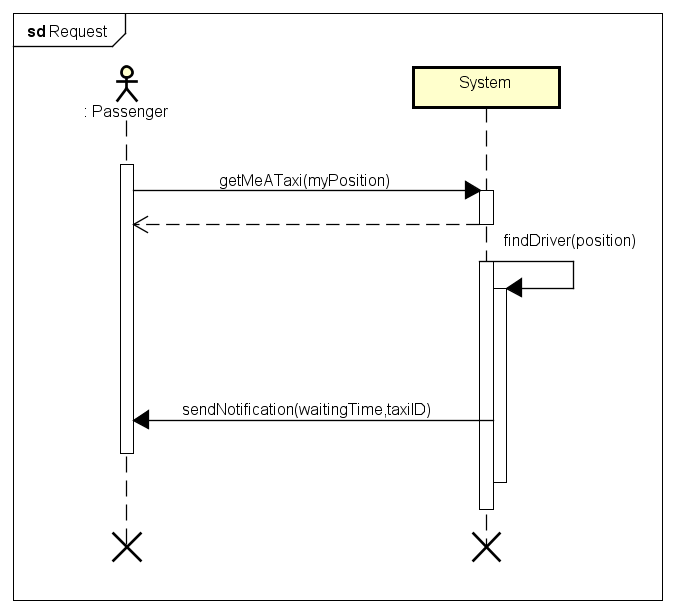
\includegraphics[keepaspectratio=true,scale=0.9]{Pictures/SDRequest}}
		\end{minipage}
	

	
	\pagebreak
	
	\paragraph{Passenger cancels a request for a taxi}
	\begin{center}
		\begin{tabular}{| l | p{9cm} |}\hline
			Actor & Passenger, Taxi driver\\\hline
			Goal & {[}G10{]} \\\hline
			Input Condition & \begin{enumerate}
								\item The user must be already logged in.
								\item The user must have a pending request for a taxi.
						   	  \end{enumerate} \\\hline
			Event Flow & The user deletes the pending ride.\\\hline
			Output Condition & \mts{} notifies the corresponding taxi driver that the job is canceled.\\\hline
			Exceptions & If the cancellation has been made after the allowed time frame the system applies a penalty fee to the user.\\\hline
		\end{tabular}
	\end{center}
	
	\pagebreak
	
	\paragraph{Passenger creates a reservation for a taxi}
	\begin{center}
		\begin{tabular}{| l | p{9cm} |}\hline
			Actor & Passenger\\\hline
			Goal & {[}G11{]} \\\hline
			Input Condition & The user must be already logged in.\\\hline
			Event Flow & The user fills in the form for the reservation of a ride customizing the parameters.\\\hline
			Output Condition & \begin{enumerate}
									\item \mts{} records the new reservation in its DB.
									\item The system notifies the user of the successful reservation.
							   \end{enumerate}\\\hline
			Exceptions & NULL\\\hline
		\end{tabular}
	\end{center}
	
	\pagebreak
	
	\paragraph{Passenger edits or deletes a reservation for a taxi}
	\begin{center}
		\begin{tabular}{| l | p{9cm} |}\hline
			Actor & Passenger\\\hline
			Goal & {[}G12{]} \\\hline
			Input Condition & \begin{enumerate}
									\item The user must be already logged in.
									\item The user must have an active reservation.
							  \end{enumerate}\\\hline
			Event Flow & The user modifies some parameters of his/her reservation, possibly also deleting it.\\\hline
			Output Condition & \begin{enumerate}
									\item \mts{} records the changes in the reservation in its DB.
									\item The system notifies the user of the successful changes.
						   	   \end{enumerate}\\\hline
			Exceptions & The system collects the penalty fee if the user deleted the ride beyond the allowed time-frame.\\\hline
		\end{tabular}
	\end{center}	
	
	\pagebreak
	
	\noindent%
	\begin{minipage}{\linewidth}
		\vspace*{-0.7cm}
		\makebox[\linewidth]{
			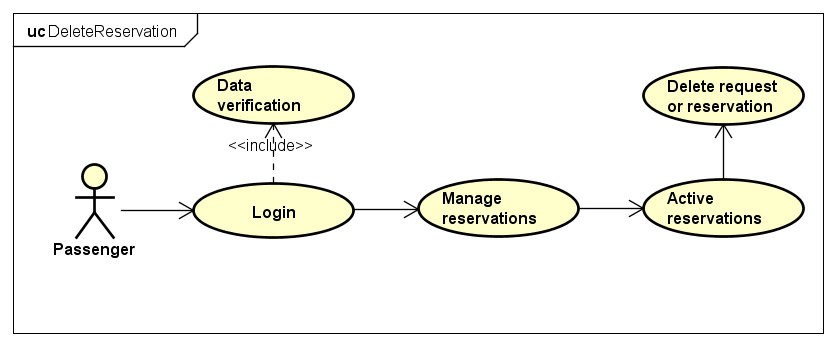
\includegraphics[keepaspectratio=true,scale=0.635]{Pictures/UCDeleteReservation}}
	\end{minipage}
	
	\vspace*{0.6cm}
	
	\noindent%
	\begin{minipage}{\linewidth}
		\vspace*{-0.75cm}
		\makebox[\linewidth]{
			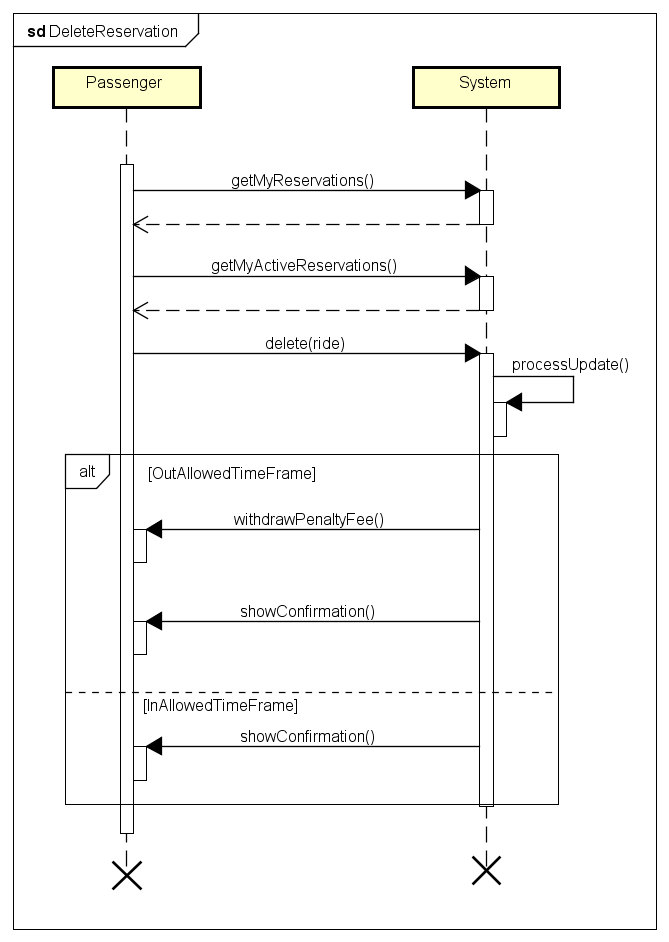
\includegraphics[keepaspectratio=true,scale=0.8]{Pictures/SDDeleteReservation}}
	\end{minipage}	

	\pagebreak
	
	\paragraph{Passenger reserves a ride with shared option}
	\begin{center}
		\begin{tabular}{| l | p{9cm} |}\hline
			Actor & Passenger\\\hline
			Goal & {[}G13{]} \\\hline
			Input Condition & The user must be already logged in.\\\hline
			Event Flow & The user fills in the form for the reservation of a ride customizing the parameters, in particular enabling the sharing of the ride.\\\hline
			Output Condition & \begin{enumerate}
				\item \mts{} records the changes in the reservation in its DB.
				\item The system notifies the user of the successful reservation.
			\end{enumerate}\\\hline
			Exceptions & NULL\\\hline
		\end{tabular}
	\end{center}	
	
	\pagebreak
	
	\paragraph{Passenger joins a shared ride}
	\begin{center}
		\begin{tabular}{| l | p{9cm} |}\hline
			Actor & Passenger\\\hline
			Goal & {[}G14{]} \\\hline
			Input Condition & \begin{enumerate}
				\item The users involved in the shared ride must be already logged in.
				\item The users must have an active reservation in which they have expressly accepted the shared ride option.
				\item The active reservation must have the same origin and destination for all the users.
			\end{enumerate}\\\hline
			Event Flow & The system recognizes the possible shared rides and insert them in the DB.\\\hline
			Output Condition & All the users involved are notified about the matching of users for shared rides, therefore they are updated on the situation of the shared ride.\\\hline
			Exceptions & NULL\\\hline
		\end{tabular}
	\end{center}	
	
	\pagebreak
	
	\paragraph{Passenger checks the history of his/her own requests}
	\begin{center}
		\begin{tabular}{| l | p{9cm} |}\hline
			Actor & Passenger\\\hline
			Goal & {[}G15{]} \\\hline
			Input Condition & The user must be already logged in.\\\hline
			Event Flow & The user accesses the page of the history of his/her own rides.\\\hline
			Output Condition & The system returns the result of the corresponding query on the DB to the user.\\\hline
			Exceptions & NULL\\\hline
		\end{tabular}
	\end{center}	
	
	\pagebreak
	
	\paragraph{Taxi driver logins to \mts{}}
	\begin{center}
		\begin{tabular}{| l | p{9cm} |}\hline
			Actor & Taxi driver\\\hline
			Goal & {[}G16{]} \\\hline
			Input Condition & The user must be already registered (inserted in the system by the administrator).\\\hline
			Event Flow & \begin{enumerate}
				\item \mts{} shows the login page.
				\item The user completes the form inserting correct username and password.
			\end{enumerate}\\\hline
			Output Condition & \begin{enumerate}
				\item \mts{} verifies the credentials of the employee and if correct shows the home page for the registered user.
				\item Guest is promoted to registered user.
			\end{enumerate}\\\hline
			Exceptions & If username and/or password are incorrect the system notifies this to the guest and shows the login page again.\\\hline
		\end{tabular}
	\end{center}
	
	\pagebreak
	
	\paragraph{Taxi driver sets his/her availability with the mobile application}
	\begin{center}
		\begin{tabular}{| l | p{9cm} |}\hline
			Actor & Taxi driver\\\hline
			Goal & {[}G17{]} \\\hline
			Input Condition & The user must be already logged in.\\\hline
			Event Flow & \begin{enumerate}
				\item \mts{} shows the home page for the driver.
				\item The user sets his/her own availability to receive job proposals as s/he prefers.
			\end{enumerate}\\\hline
			Output Condition & The system receives the setting of the user and operates accordingly.\\\hline
			Exceptions & NULL\\\hline
		\end{tabular}
	\end{center}
	
	\pagebreak
	
	\paragraph{Taxi driver accepts or rejects a job with the mobile application}
	\begin{center}
		\begin{tabular}{| l | p{9cm} |}\hline
			Actor & Taxi driver\\\hline
			Goal & {[}G18{]} \\\hline
			Input Condition & The user must be already logged in.\\\hline
			Event Flow & \begin{enumerate}
				\item \mts{} shows the home page for the driver.
				\item \mts{} notifies the user about a job proposal that could fit him/her.	
				\item The user chooses whether accepting or rejecting the proposal.
			\end{enumerate}\\\hline
			Output Condition & The system receives the setting of the user and operates accordingly.\\\hline
			Exceptions & NULL\\\hline
		\end{tabular}
	\end{center}
	
	
	\pagebreak
	\noindent%
	\begin{minipage}{\linewidth}
		\vspace*{-0.5cm}
		\makebox[\linewidth]{
			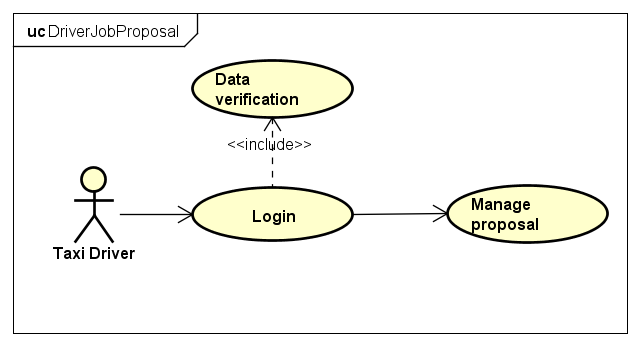
\includegraphics[keepaspectratio=true,scale=0.86]{Pictures/UCDriverJobProposal}}
	\end{minipage}
	
	\vspace*{0.5cm}
	
			\noindent%
			\begin{minipage}{\linewidth}
				\vspace*{-0.7cm}
				\makebox[\linewidth]{
					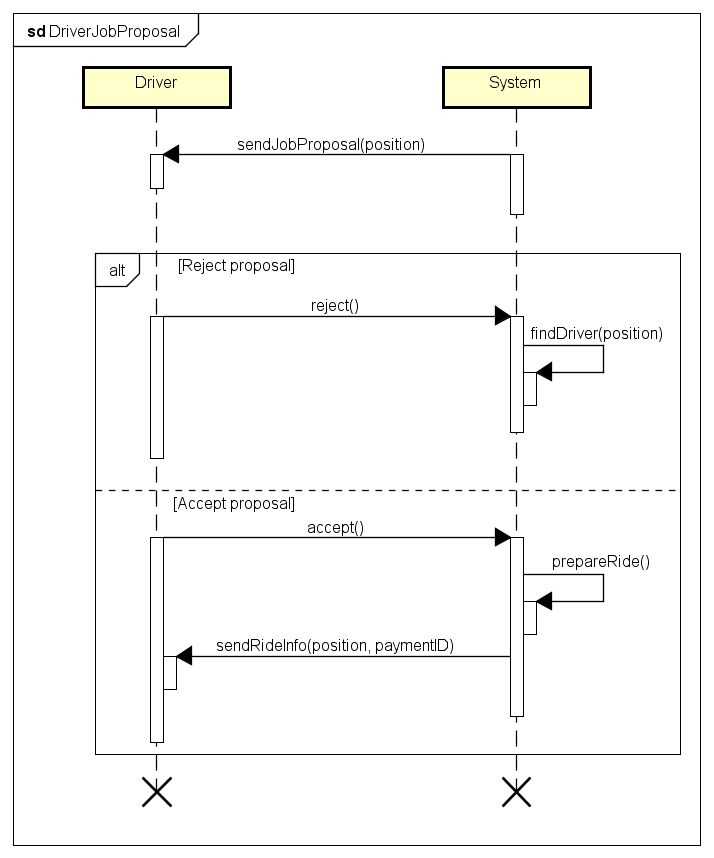
\includegraphics[keepaspectratio=true,scale=0.77]{Pictures/SDDriverJobProposal}}
			\end{minipage}	
	
	\pagebreak
	
	\paragraph{System administrator manages the drivers list}
	\begin{center}
		\begin{tabular}{| l | p{9cm} |}\hline
			Actor & Administrator\\\hline
			Goal & {[}G19{]} \\\hline
			Input Condition & The user must be already logged in.\\\hline
			Event Flow & \begin{enumerate}
				\item \mts{} shows the home page for the administrator.
				\item The user accesses the function to manage the taxi drivers.	
				\item The system shows the list of drivers.
				\item The user decides to add, modify or delete a driver.
			\end{enumerate}\\\hline
			Output Condition & The system receives the setting of the user and operates accordingly.\\\hline
			Exceptions & NULL\\\hline
		\end{tabular}
	\end{center}
	
		\pagebreak
		\noindent%
		\begin{minipage}{\linewidth}
			\vspace*{-0.2cm}
			\makebox[\linewidth]{
				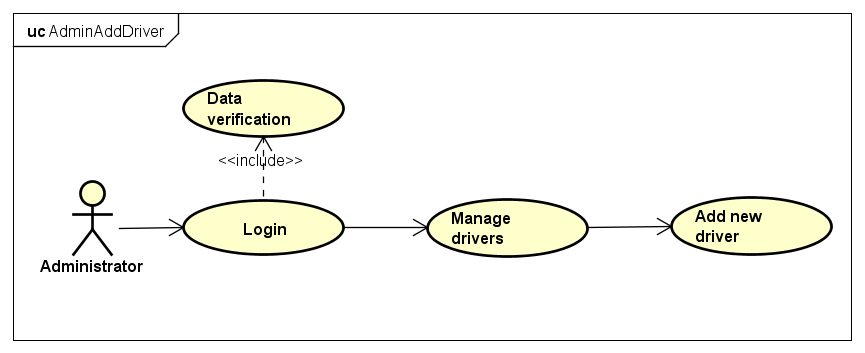
\includegraphics[keepaspectratio=true,scale=0.75]{Pictures/UCAdminAddDriver}}
		\end{minipage}
		
		\vspace*{1.1cm}
		
		\noindent%
		\begin{minipage}{\linewidth}
			\vspace*{-0.7cm}
			\makebox[\linewidth]{
				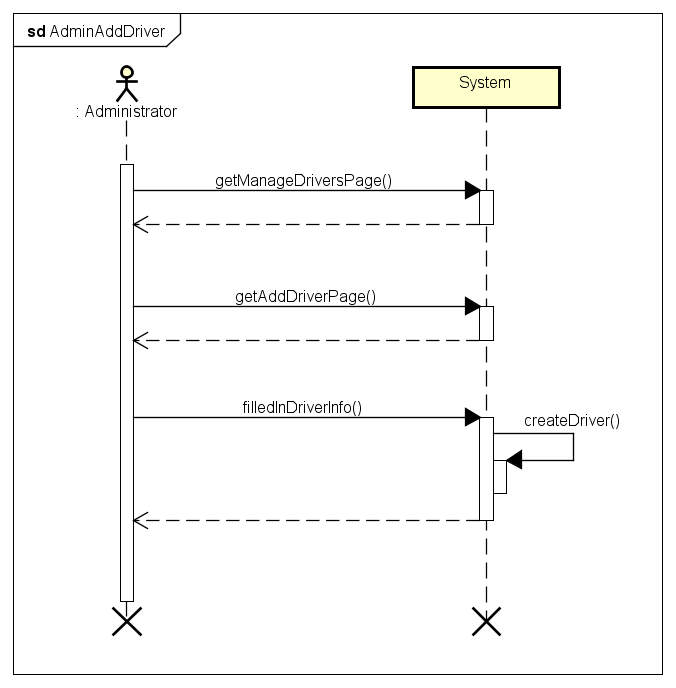
\includegraphics[keepaspectratio=true,scale=0.96]{Pictures/SDAdminAddDriver}}
		\end{minipage}	
	
	\pagebreak
	
	\paragraph{System administrator monitors the situation from the control center view}
	\begin{center}
		\begin{tabular}{| l | p{9cm} |}\hline
			Actor & Administrator\\\hline
			Goal & {[}G20{]} \\\hline
			Input Condition & The user must be already logged in.\\\hline
			Event Flow & \begin{enumerate}
				\item \mts{} shows the home page for the administrator.
				\item The user accesses system monitor.	
			\end{enumerate}\\\hline
			Output Condition & The system shows the current situation of the service.\\\hline
			Exceptions & NULL\\\hline
		\end{tabular}
	\end{center}
	
	\pagebreak		
	
	
	
%		\newgeometry{left=1cm,bottom=1cm,right=1cm,top=1cm}



%	\thispagestyle{empty}
%%	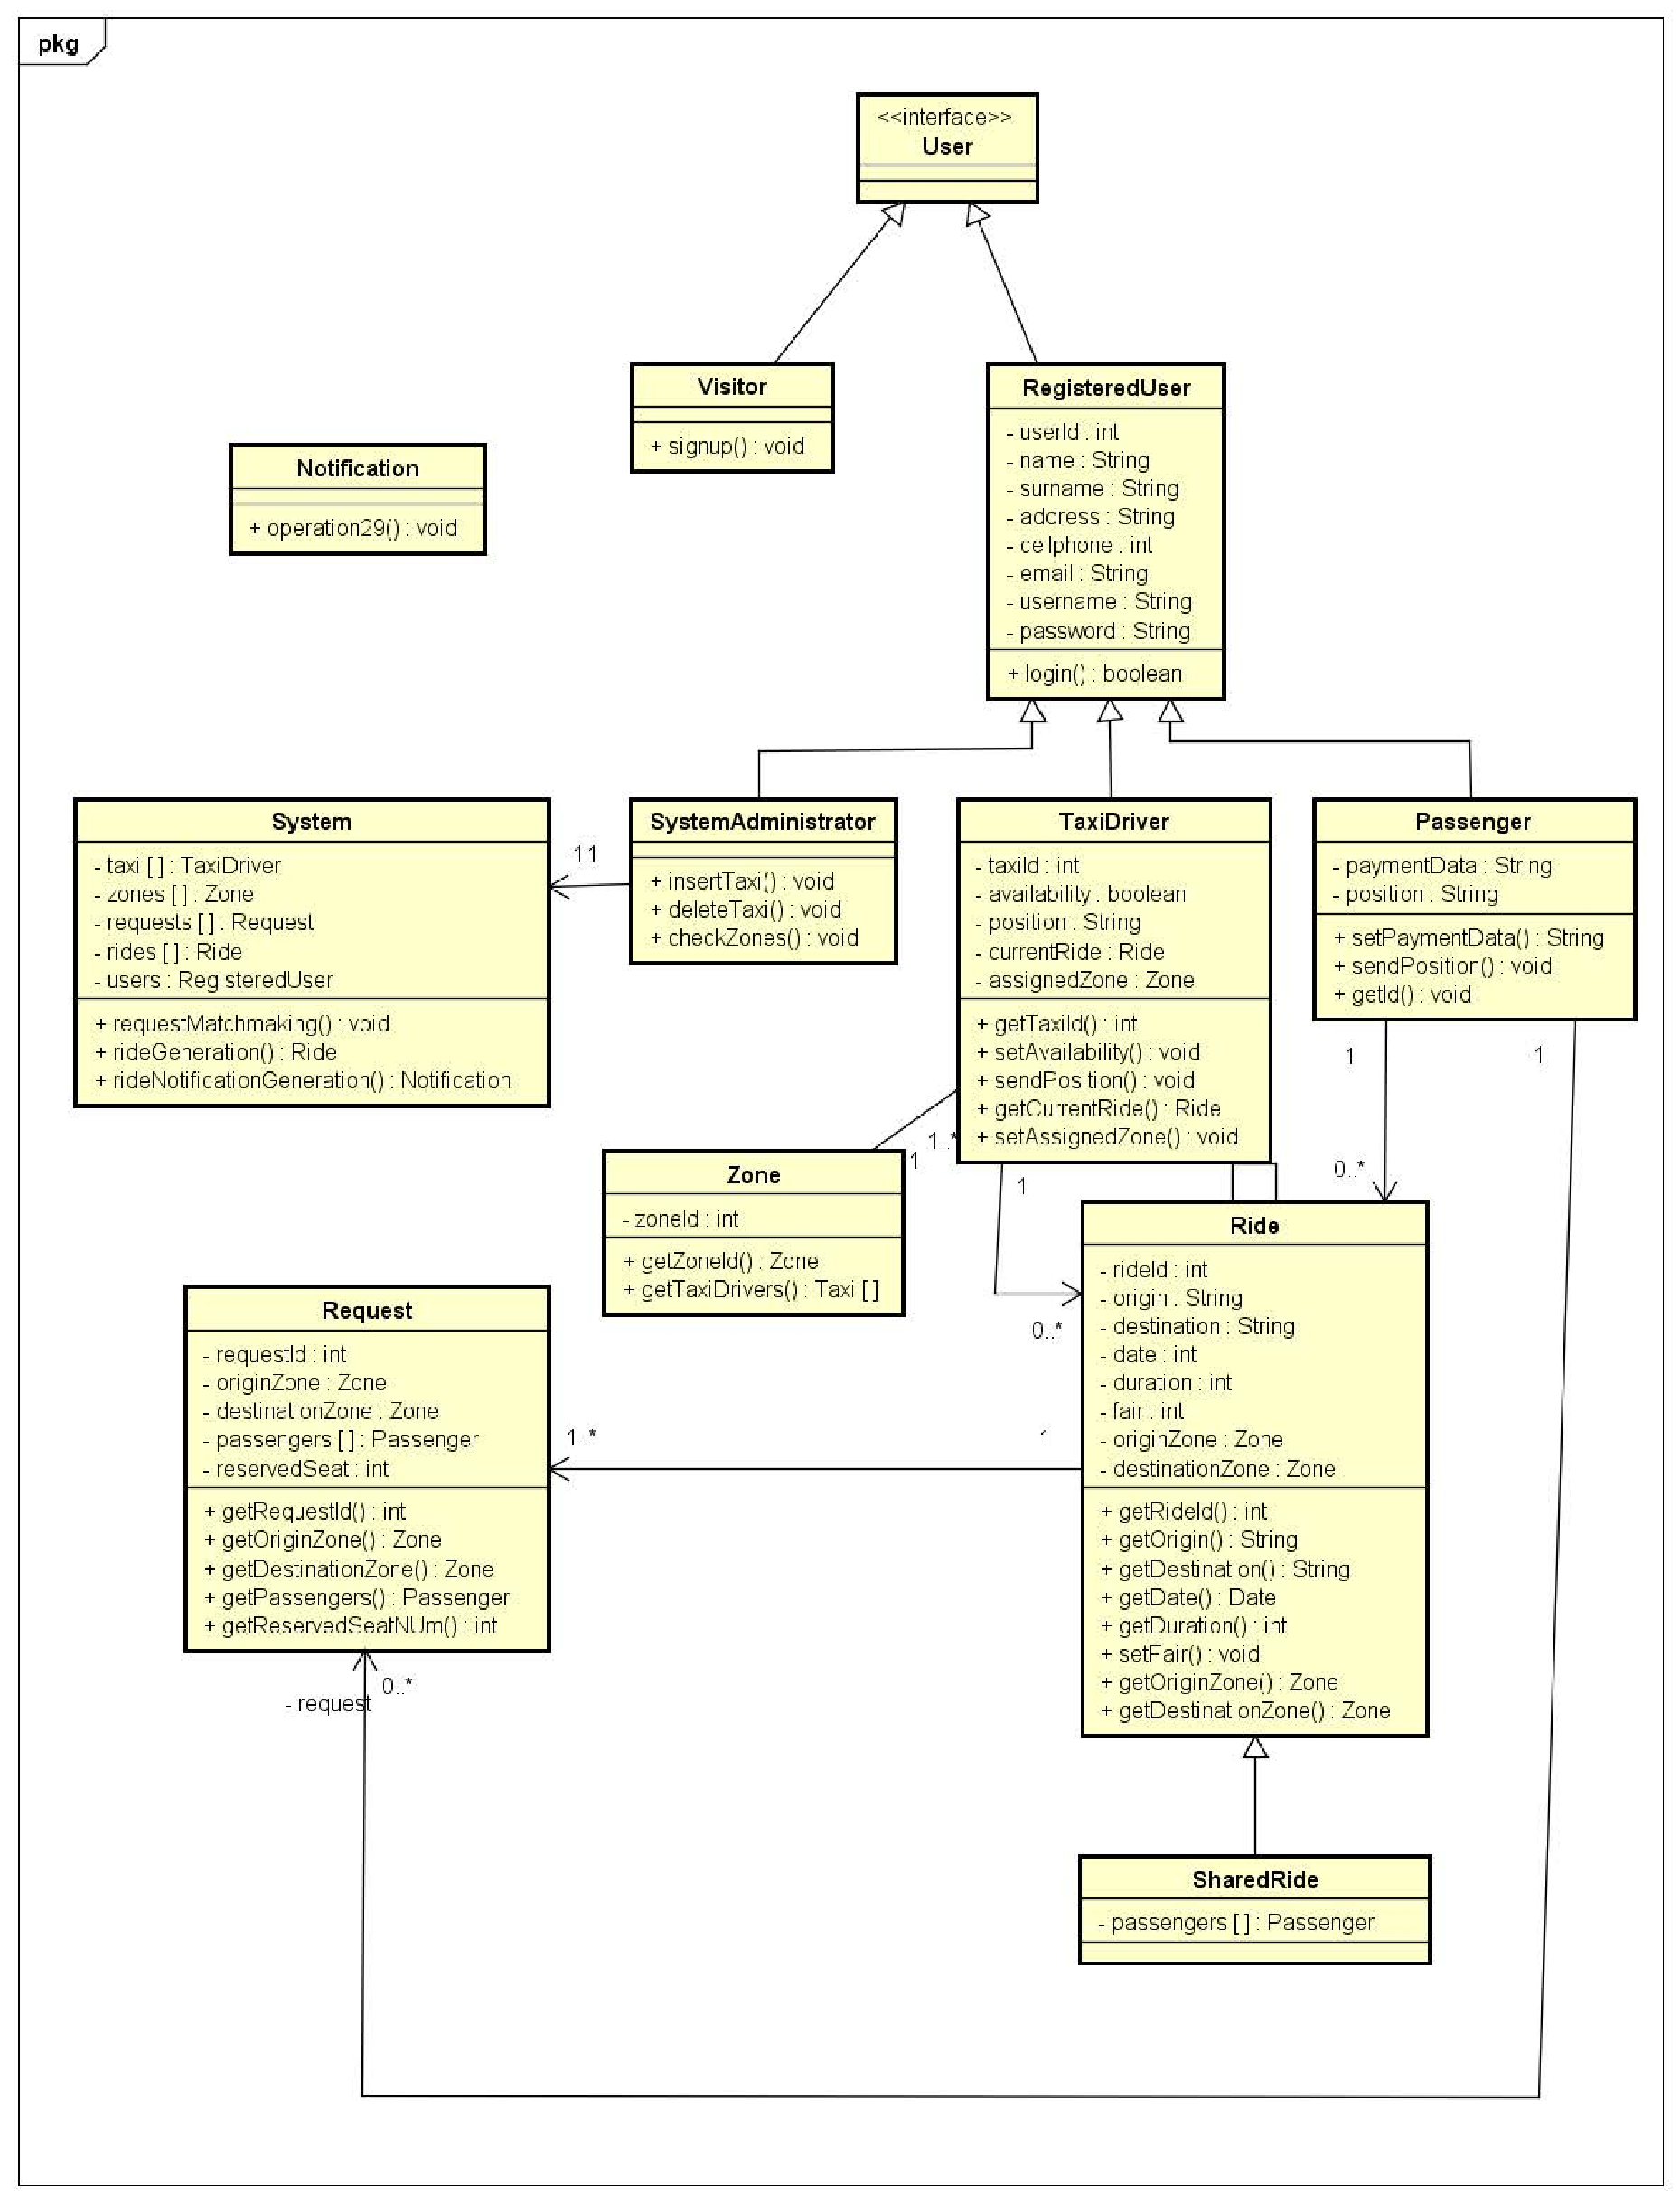
\includepdf{Pictures/ClassDiagram.pdf}
%	\AddToShipoutPictureBG*{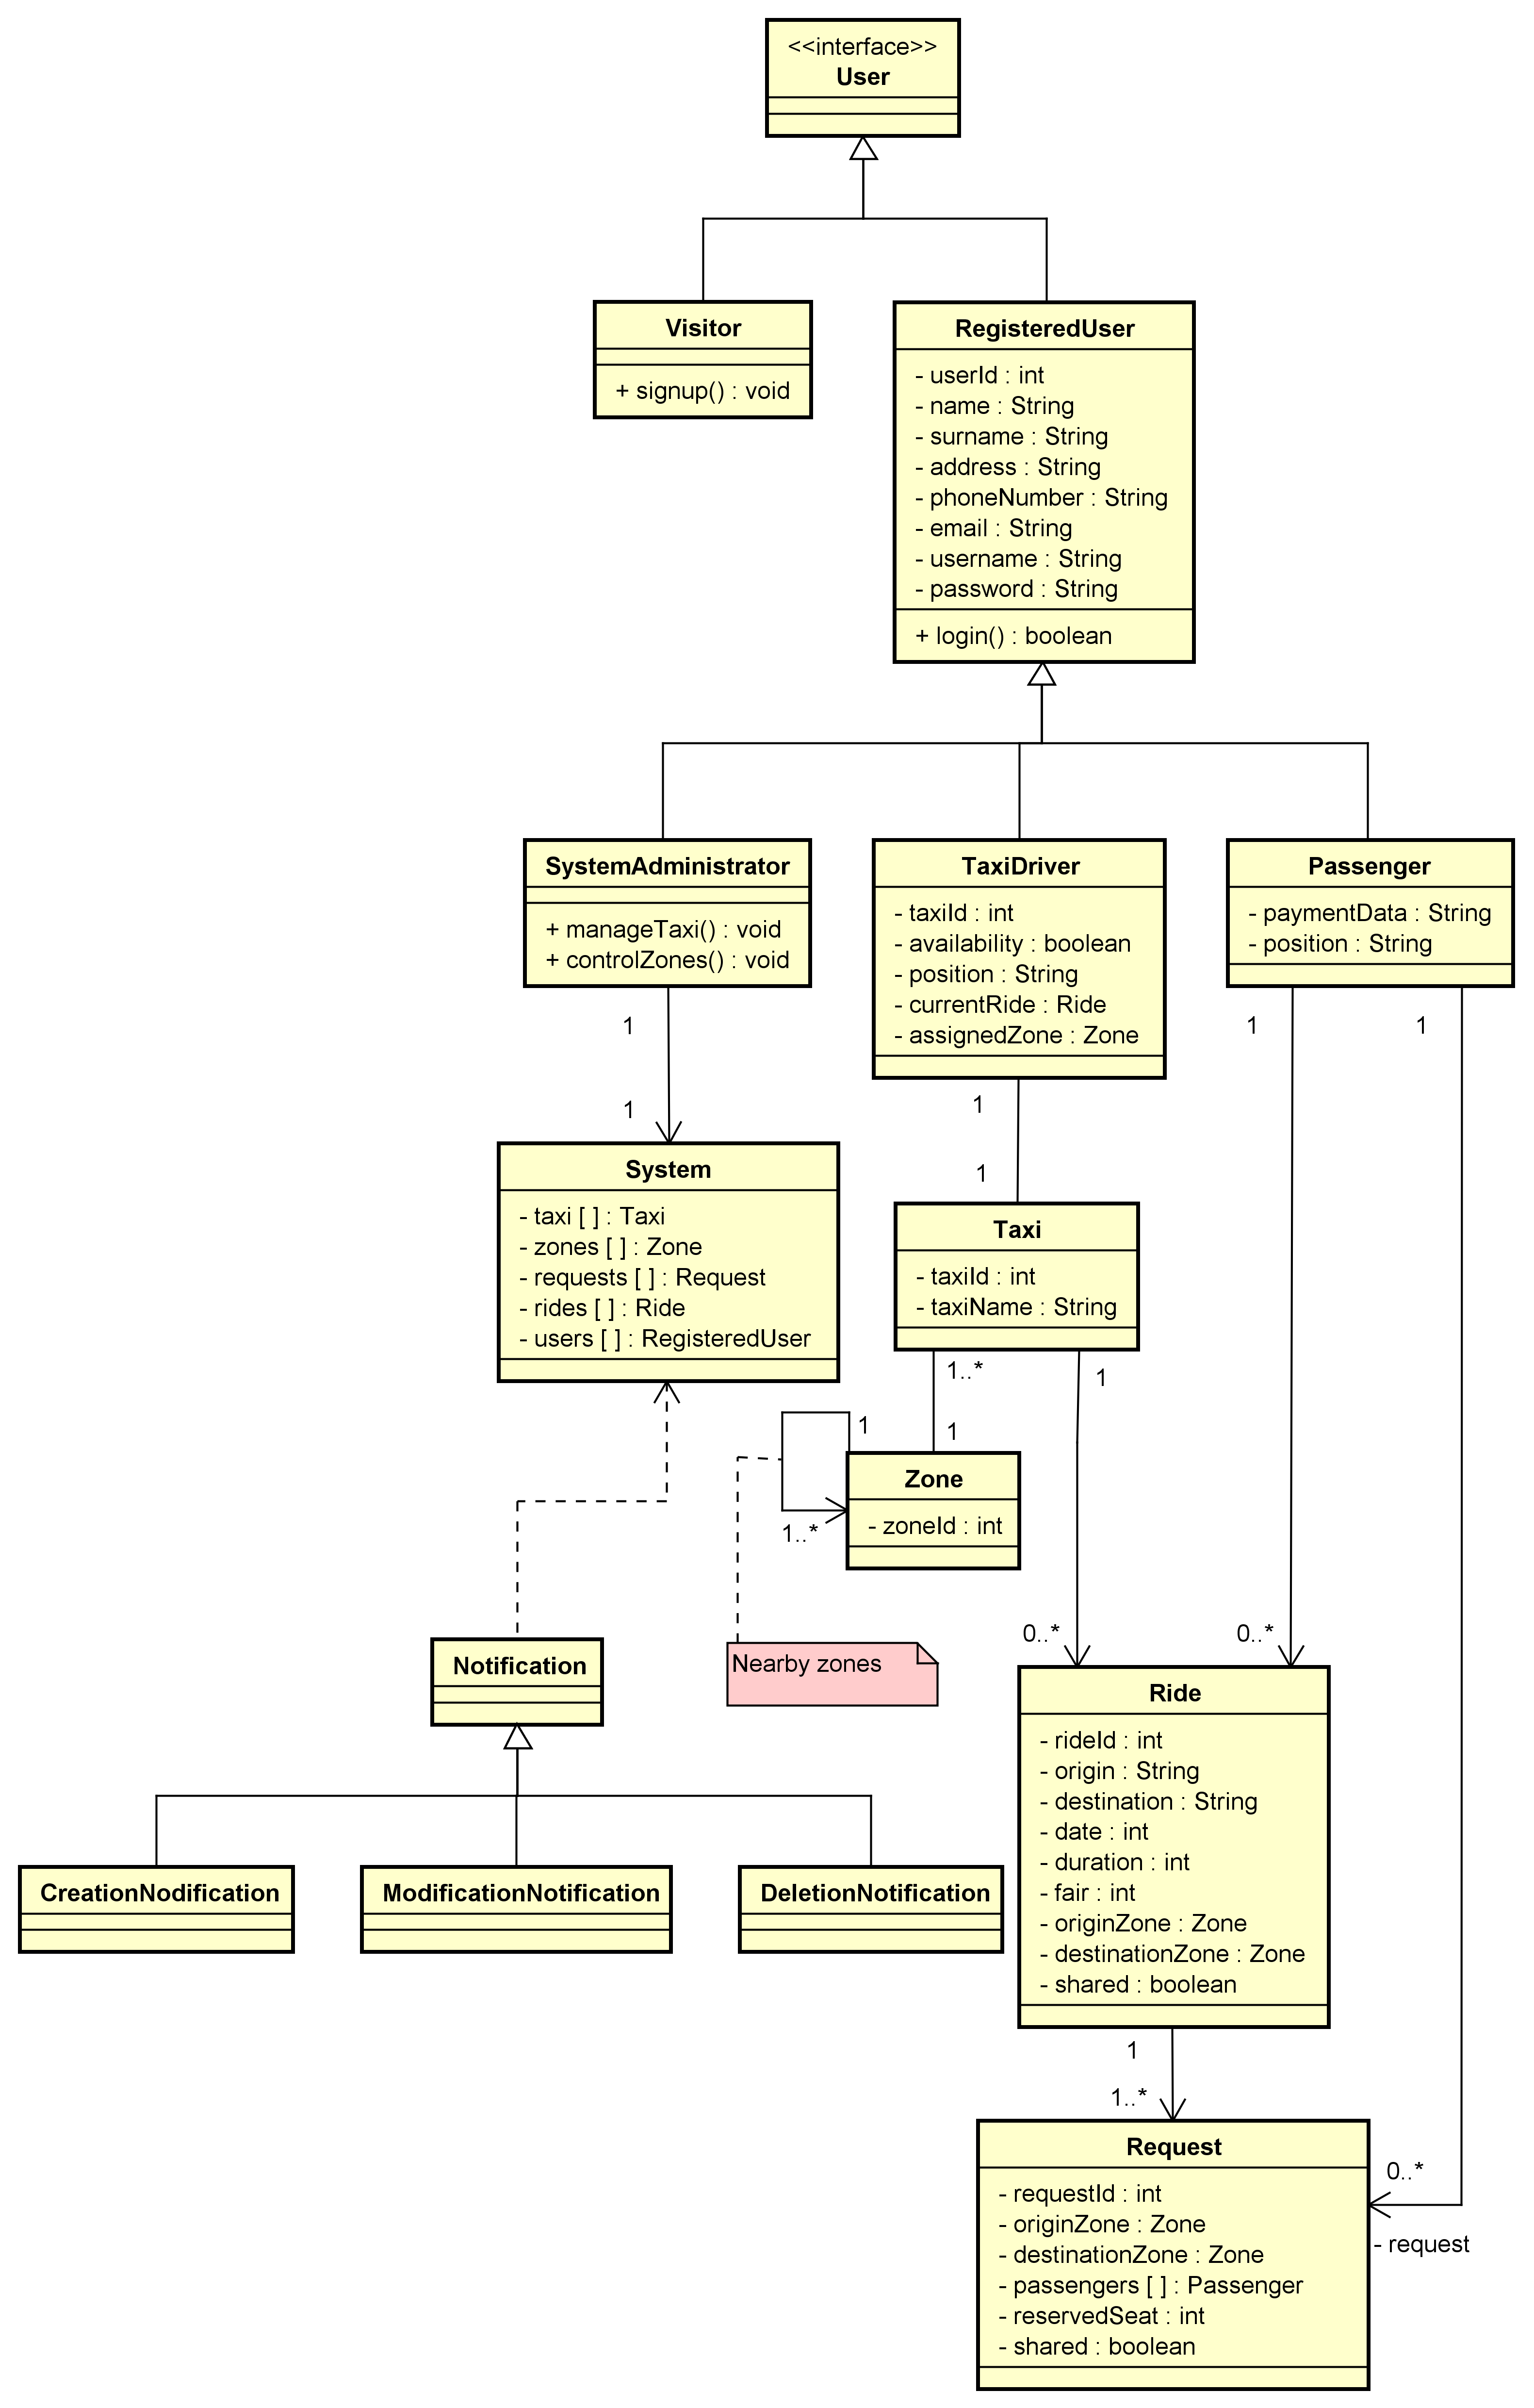
\includegraphics[width=\paperwidth,height=\paperheight]{Pictures/ClassDiagram}}
	
		\vspace*{-1.25cm}
	\subsubsection{Class Diagrams}		
		\noindent%
		\begin{minipage}{\linewidth}
			\vspace*{-0.35cm}
			\makebox[\linewidth]{
			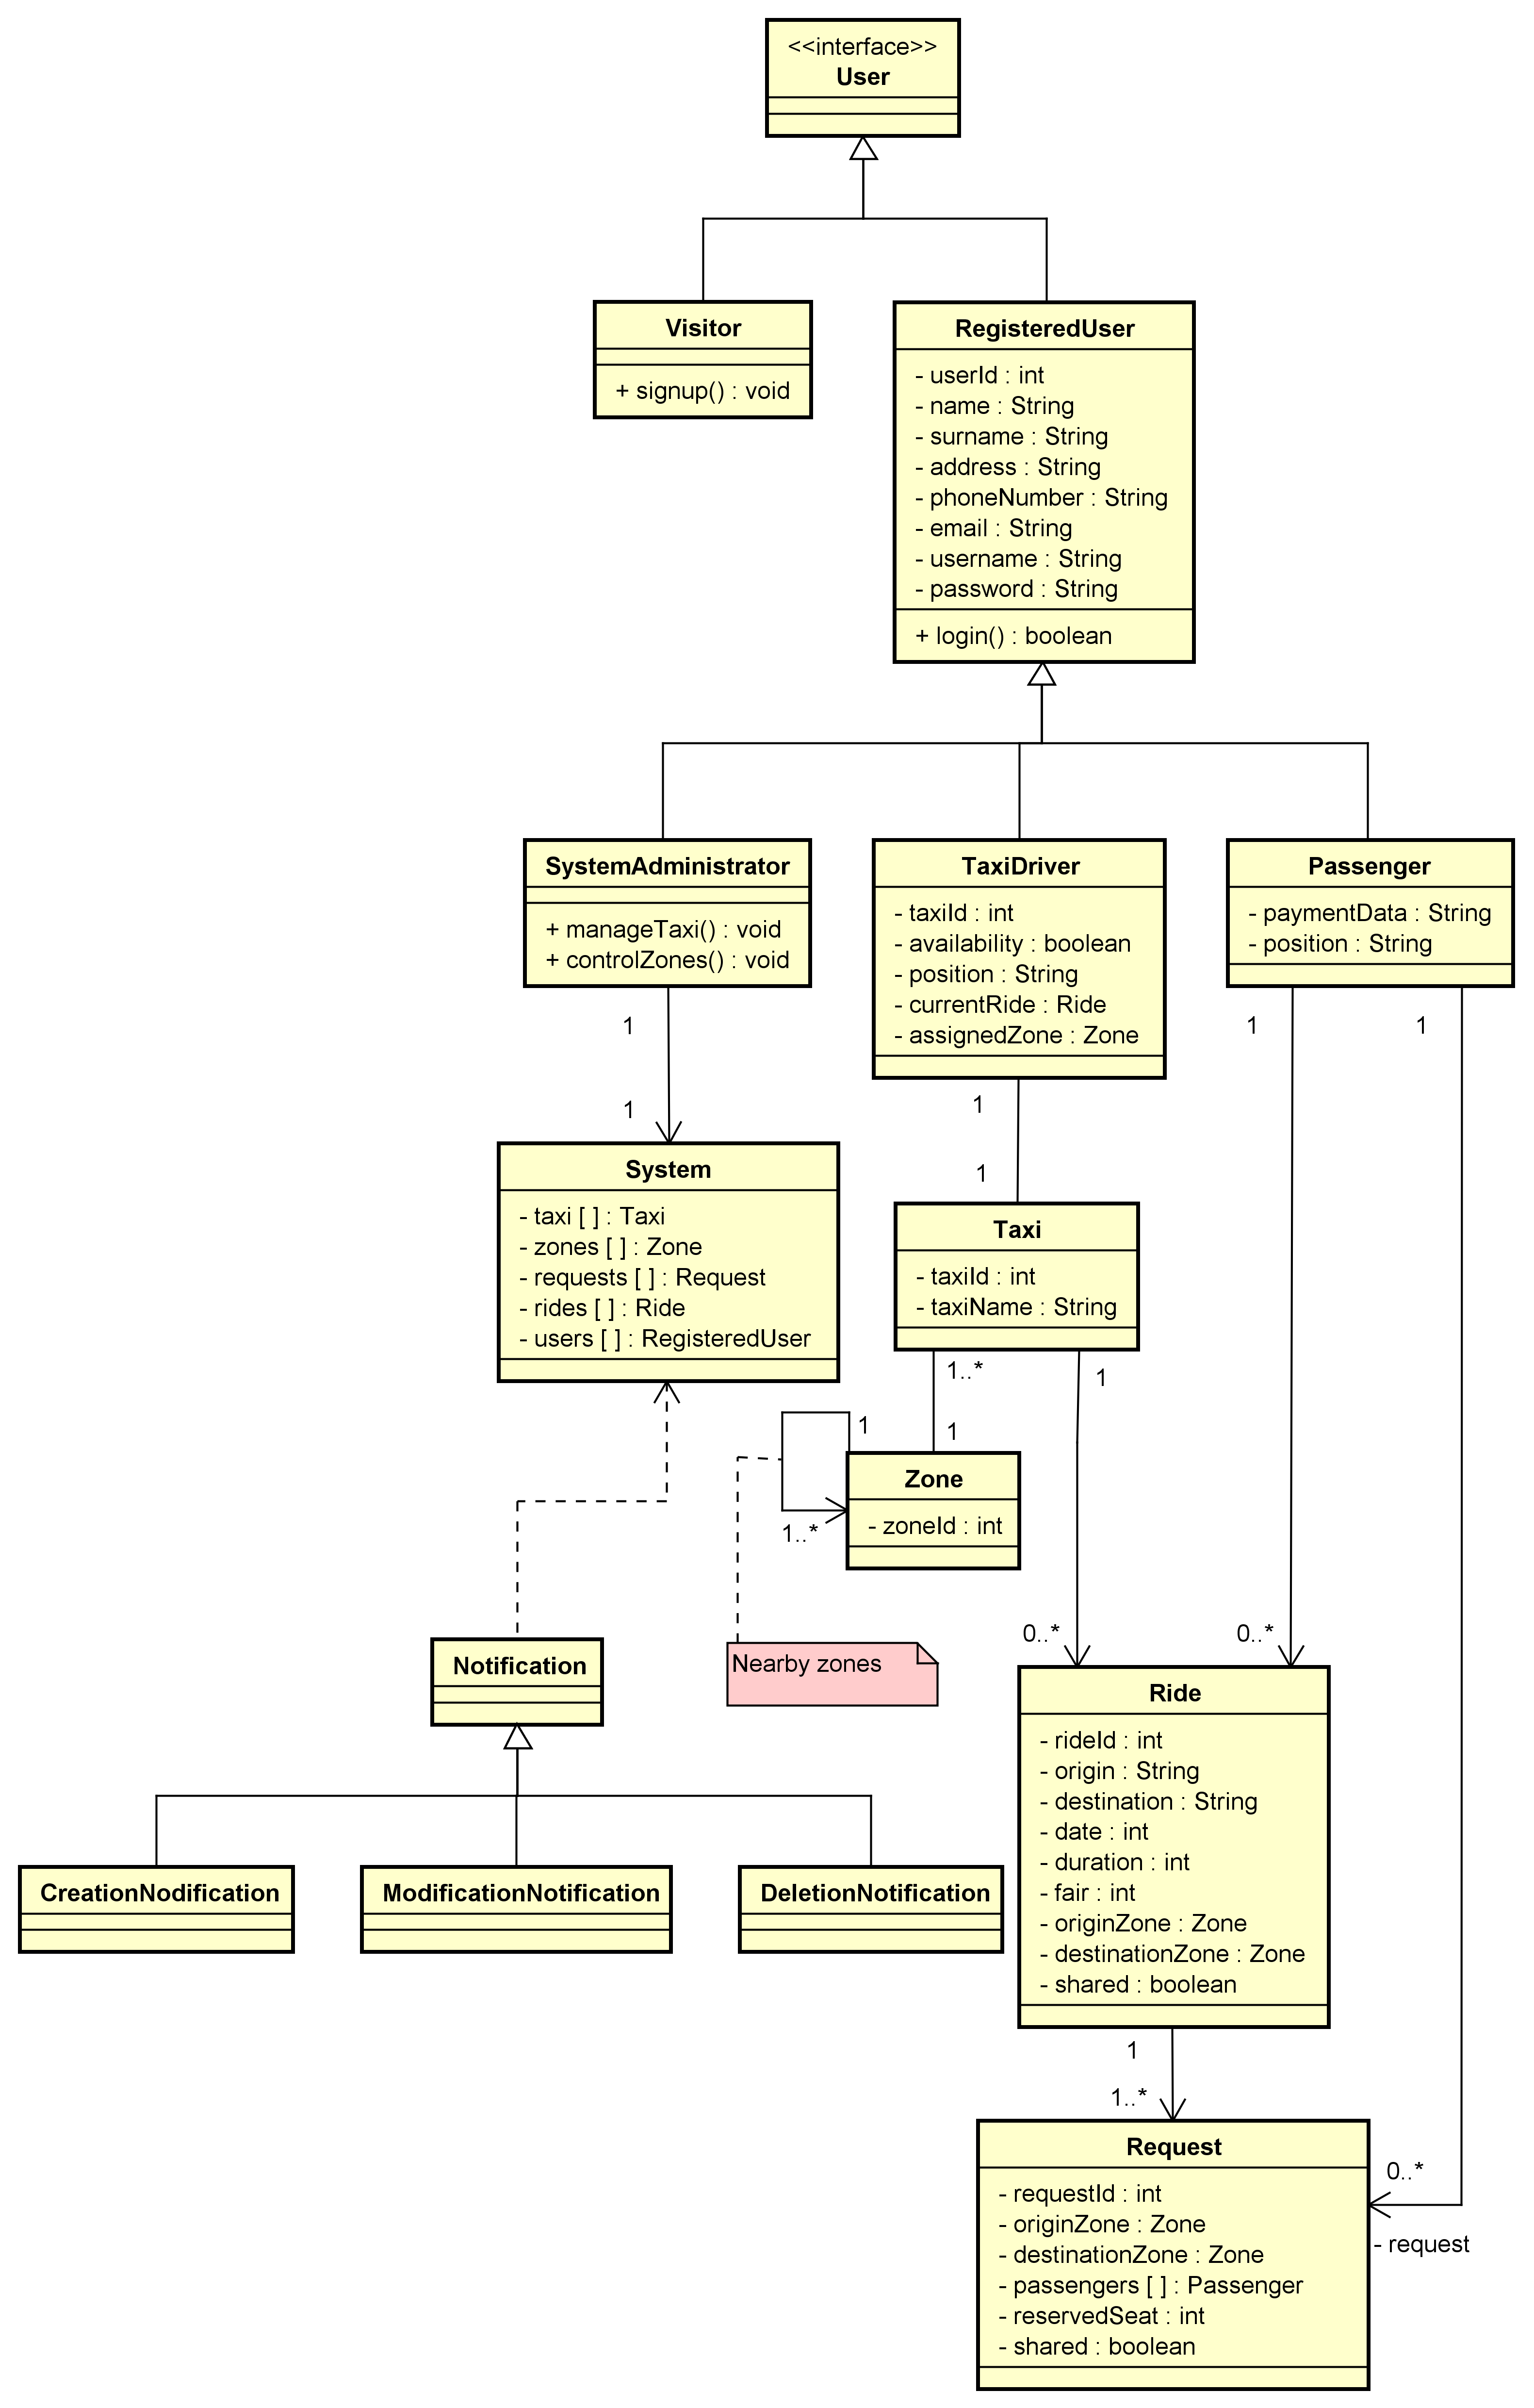
\includegraphics[keepaspectratio=true,scale=0.57]{Pictures/ClassDiagram}}
		\end{minipage}	

%\begin{figure}
%	
%	\begin{center}
%
%%		\subsubsection{Class Diagrams}
%%		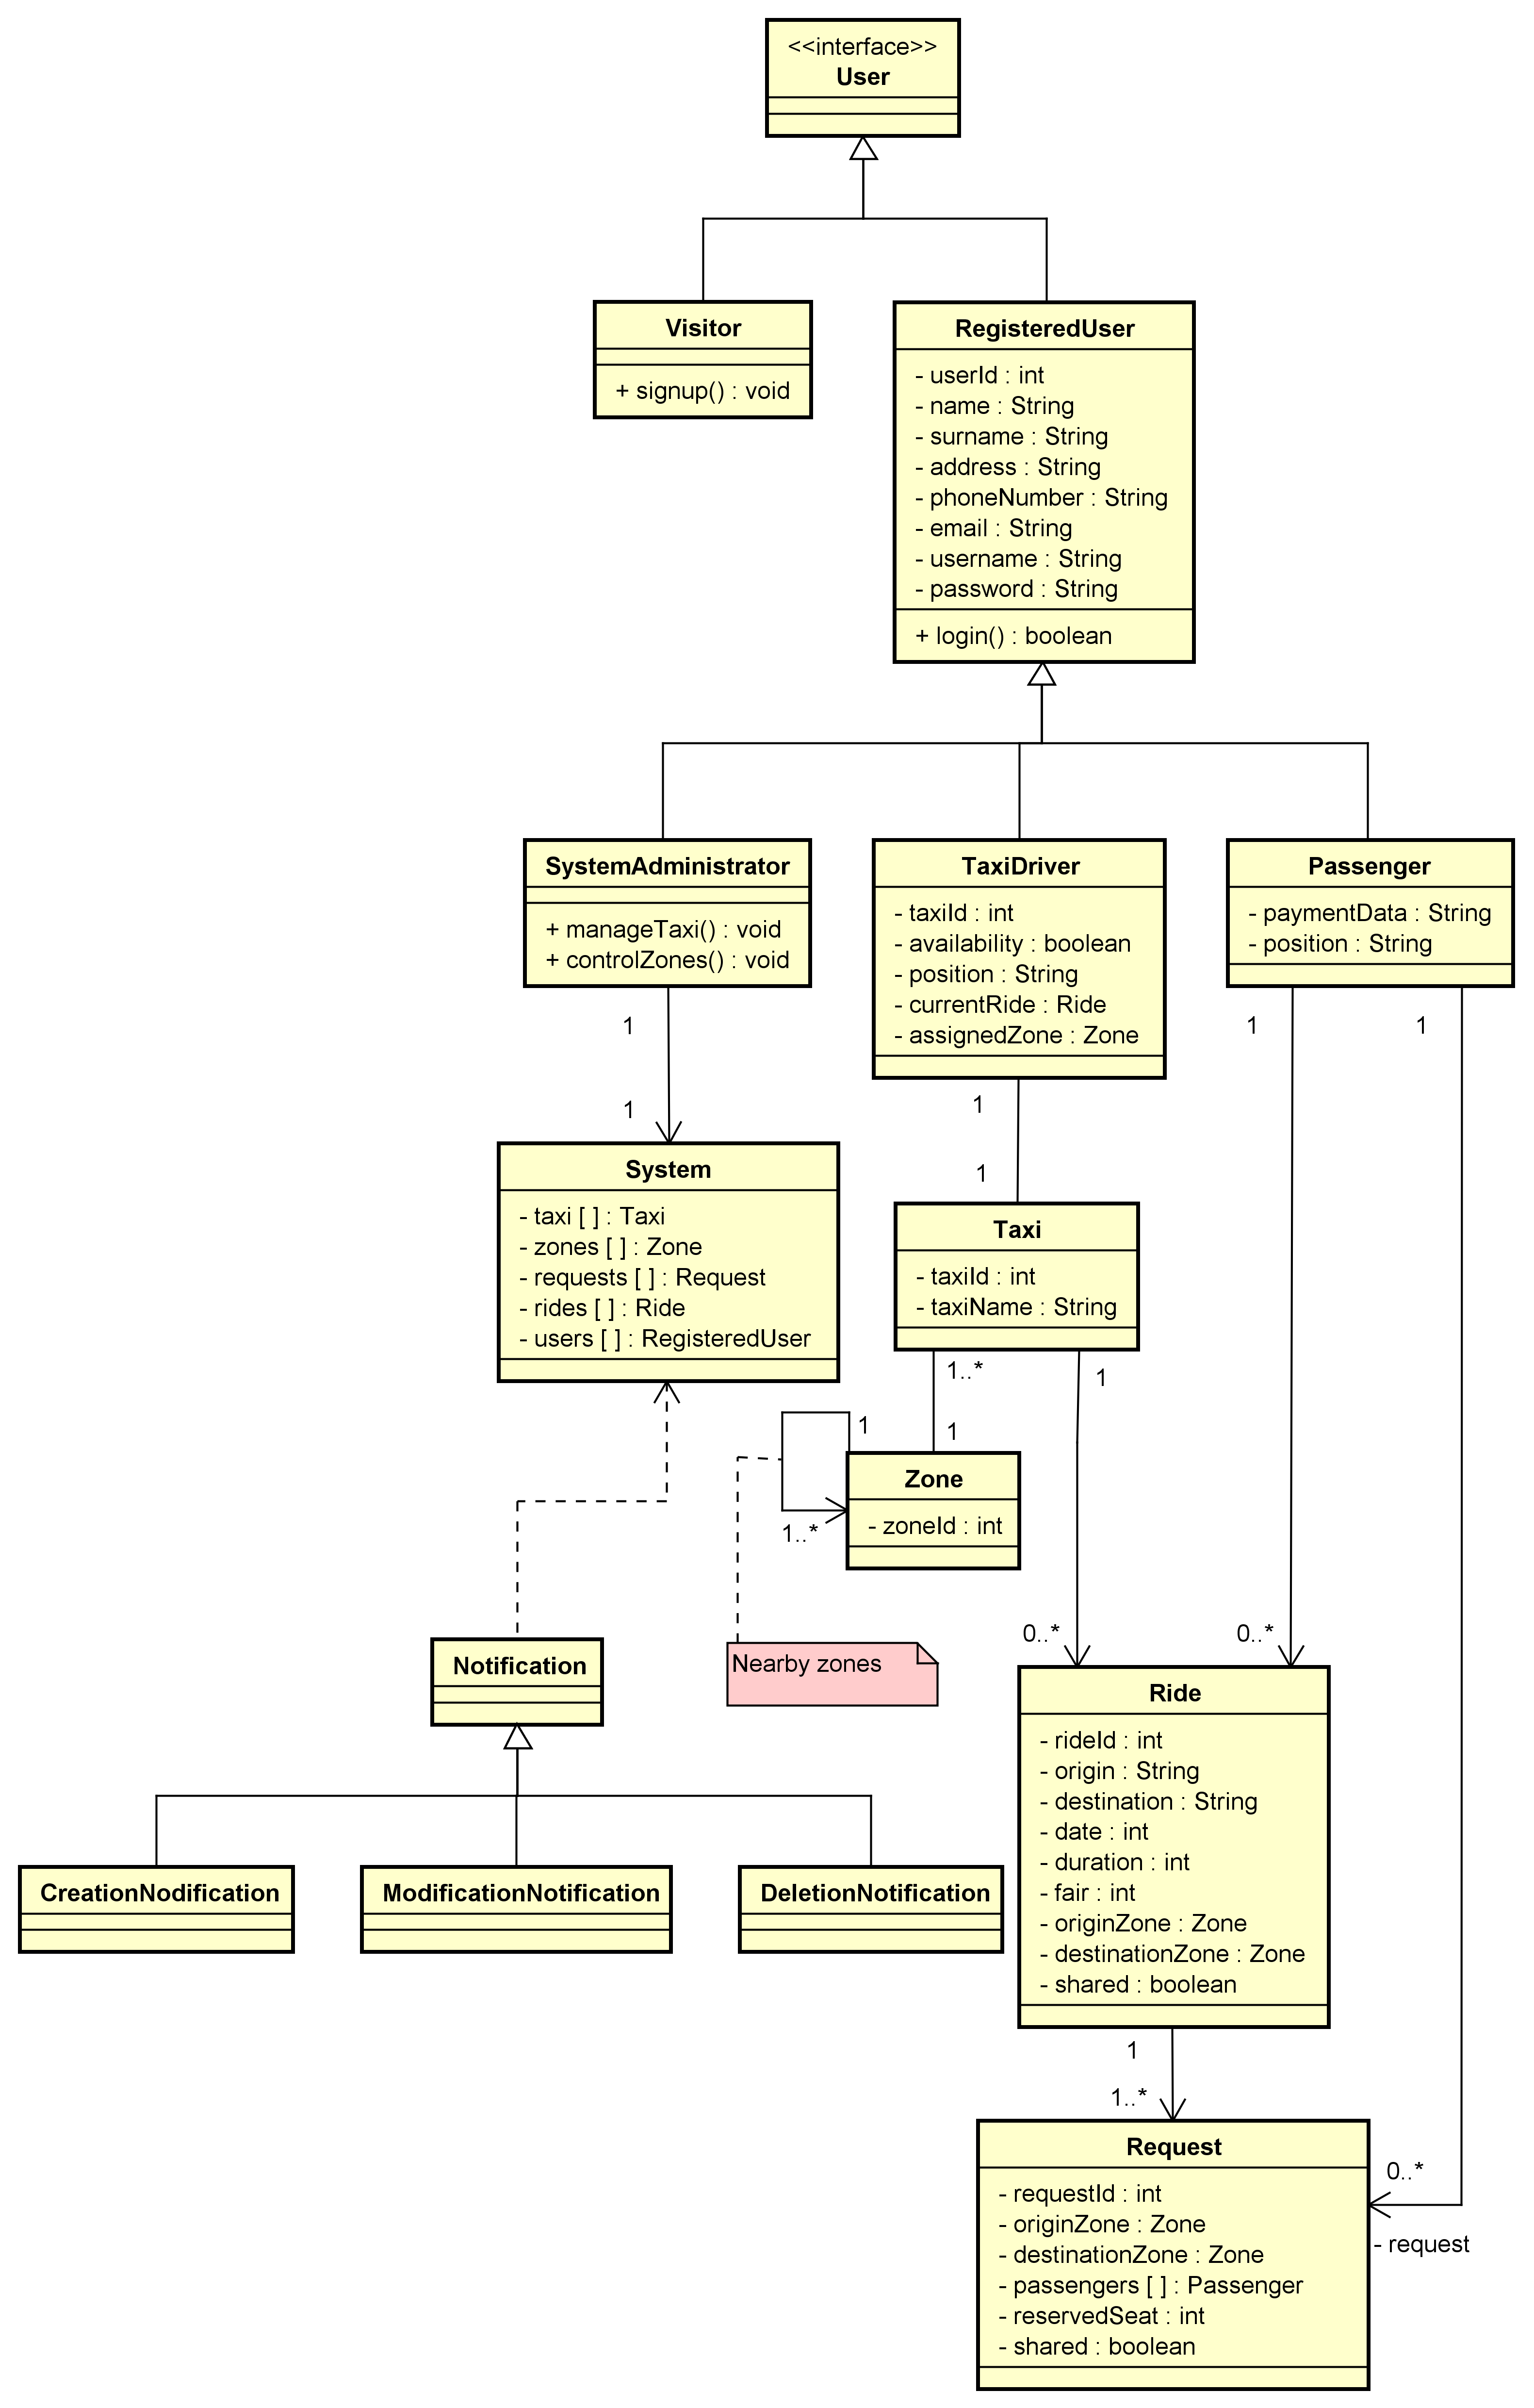
\includegraphics[width=\paperwidth,height=\paperheight]{Pictures/ClassDiagram}
%\makebox[\linewidth]{
%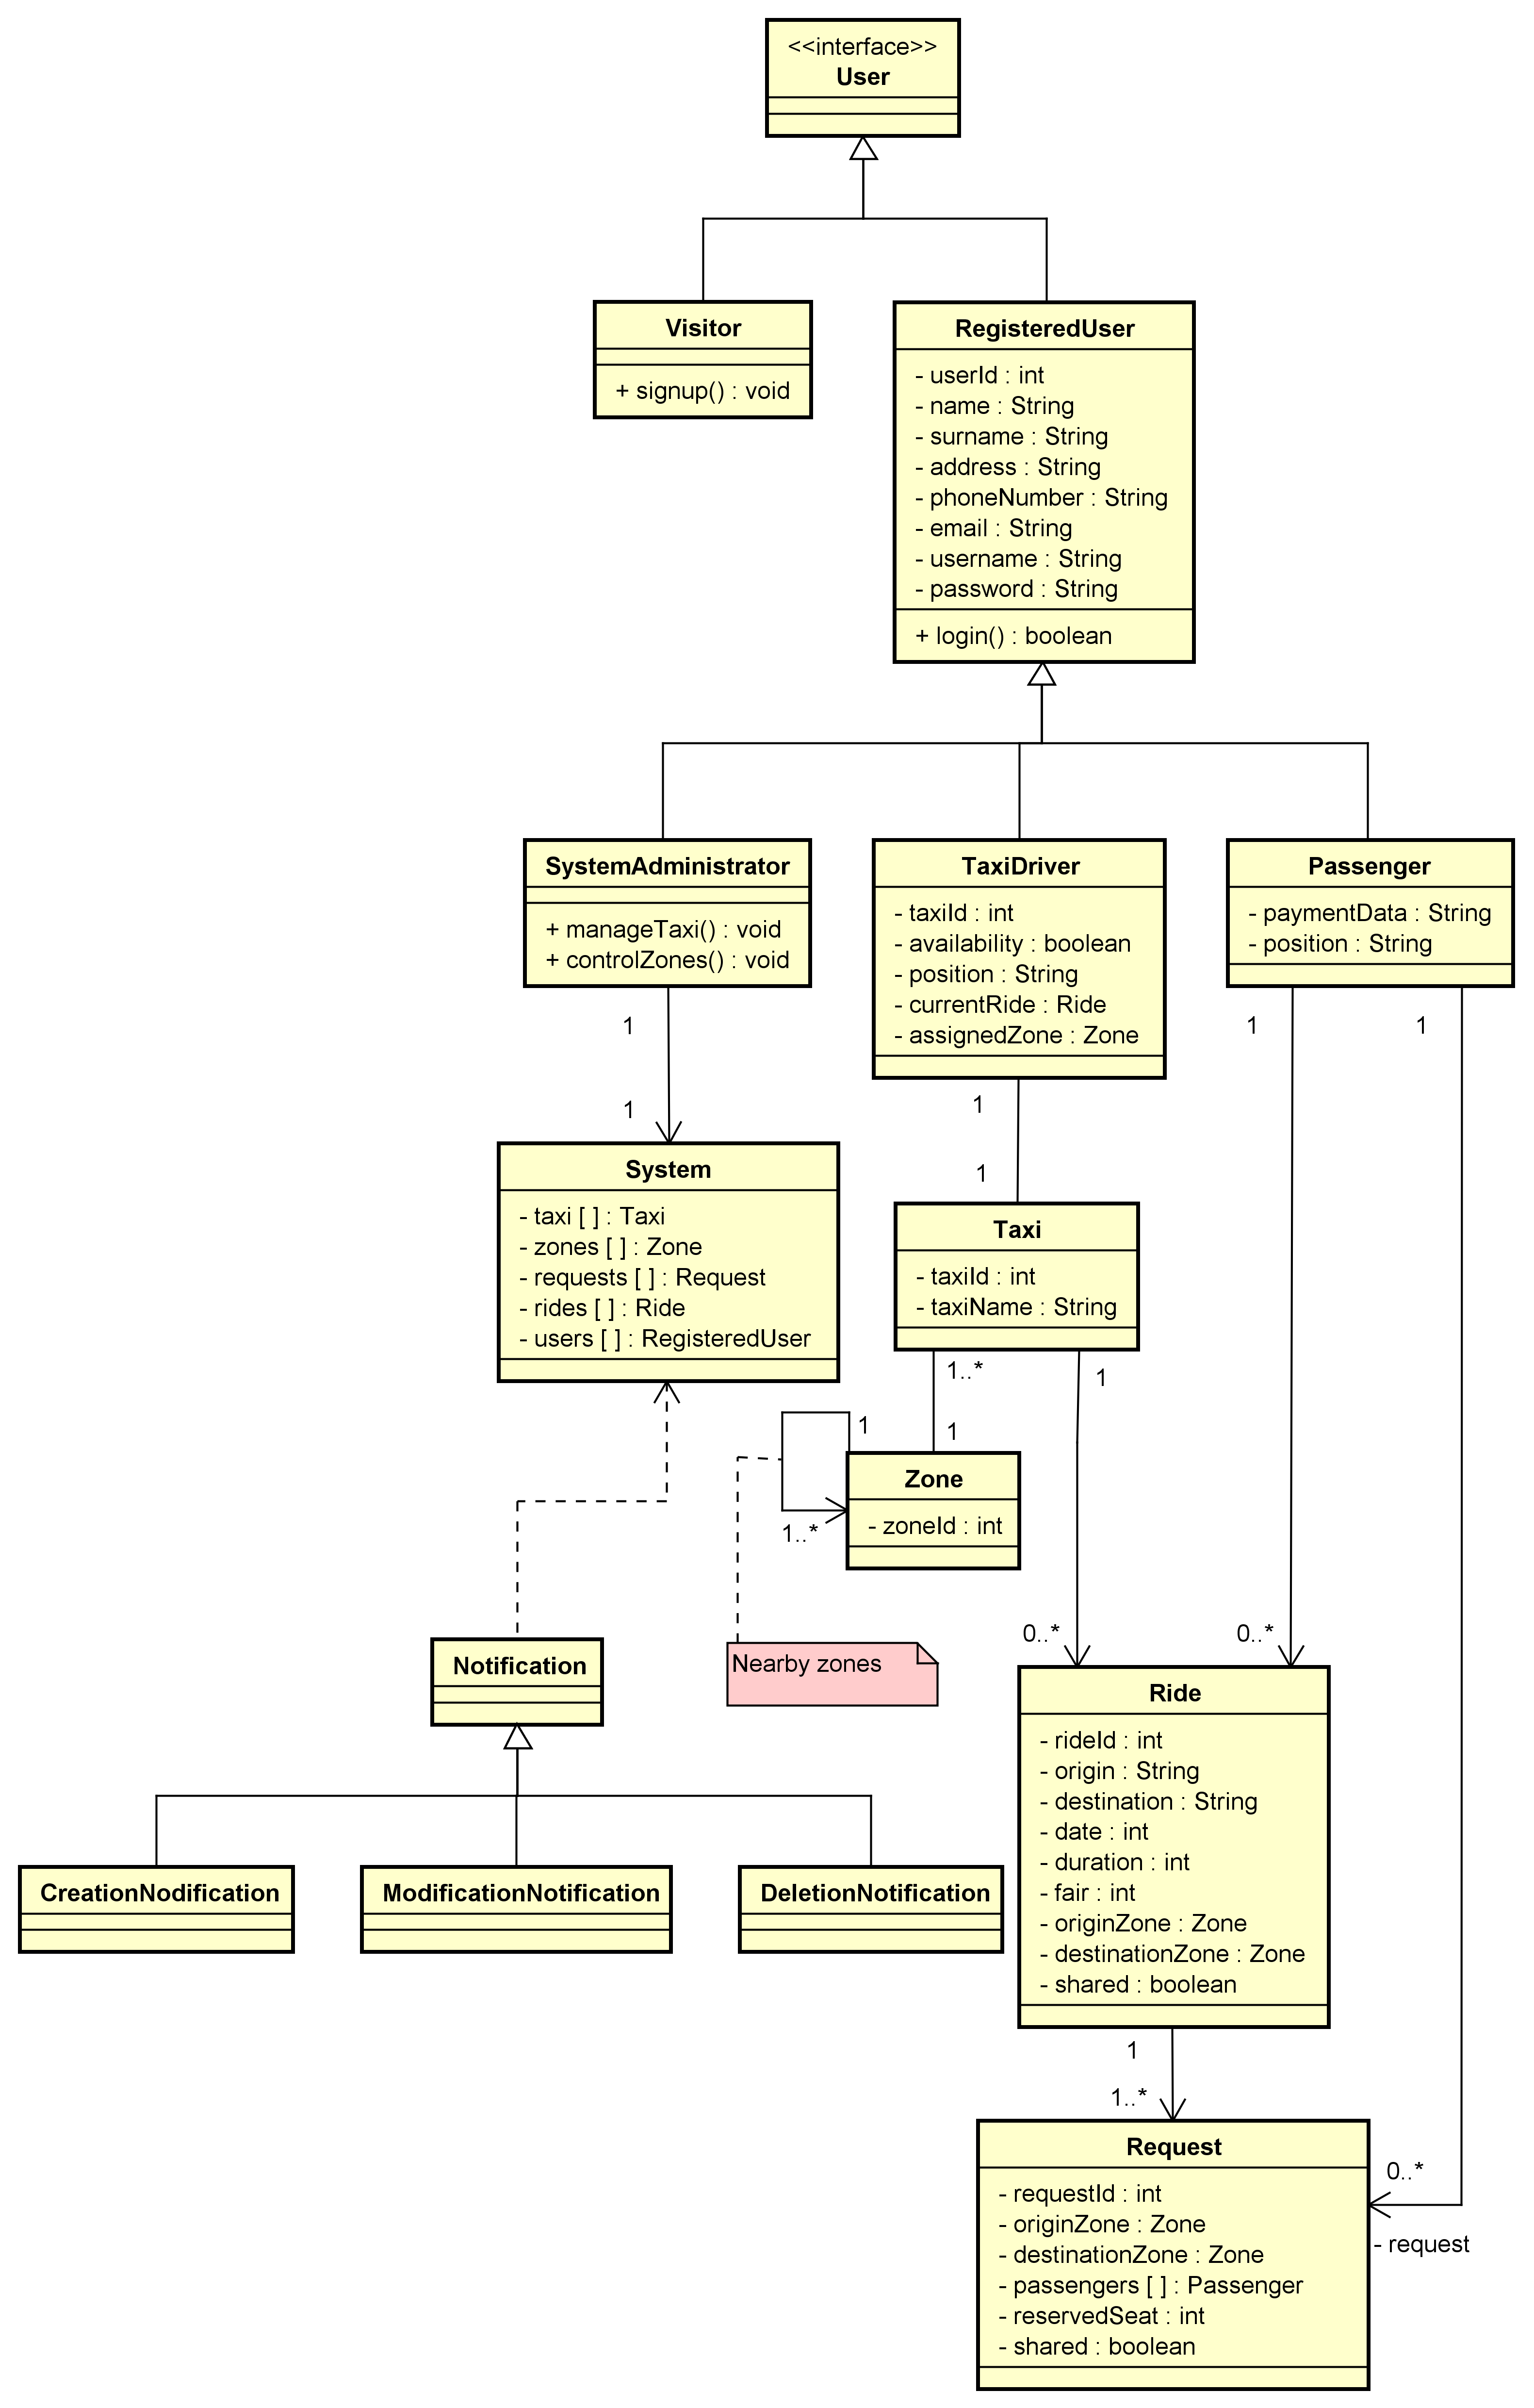
\includegraphics[keepaspectratio=true,scale=0.57]{Pictures/ClassDiagram}}
%	\end{center}
%\end{figure}	
	
	
%	\afterpage{\clearpage}
%	\vfill
%		\begin{center}
%%			\centerline{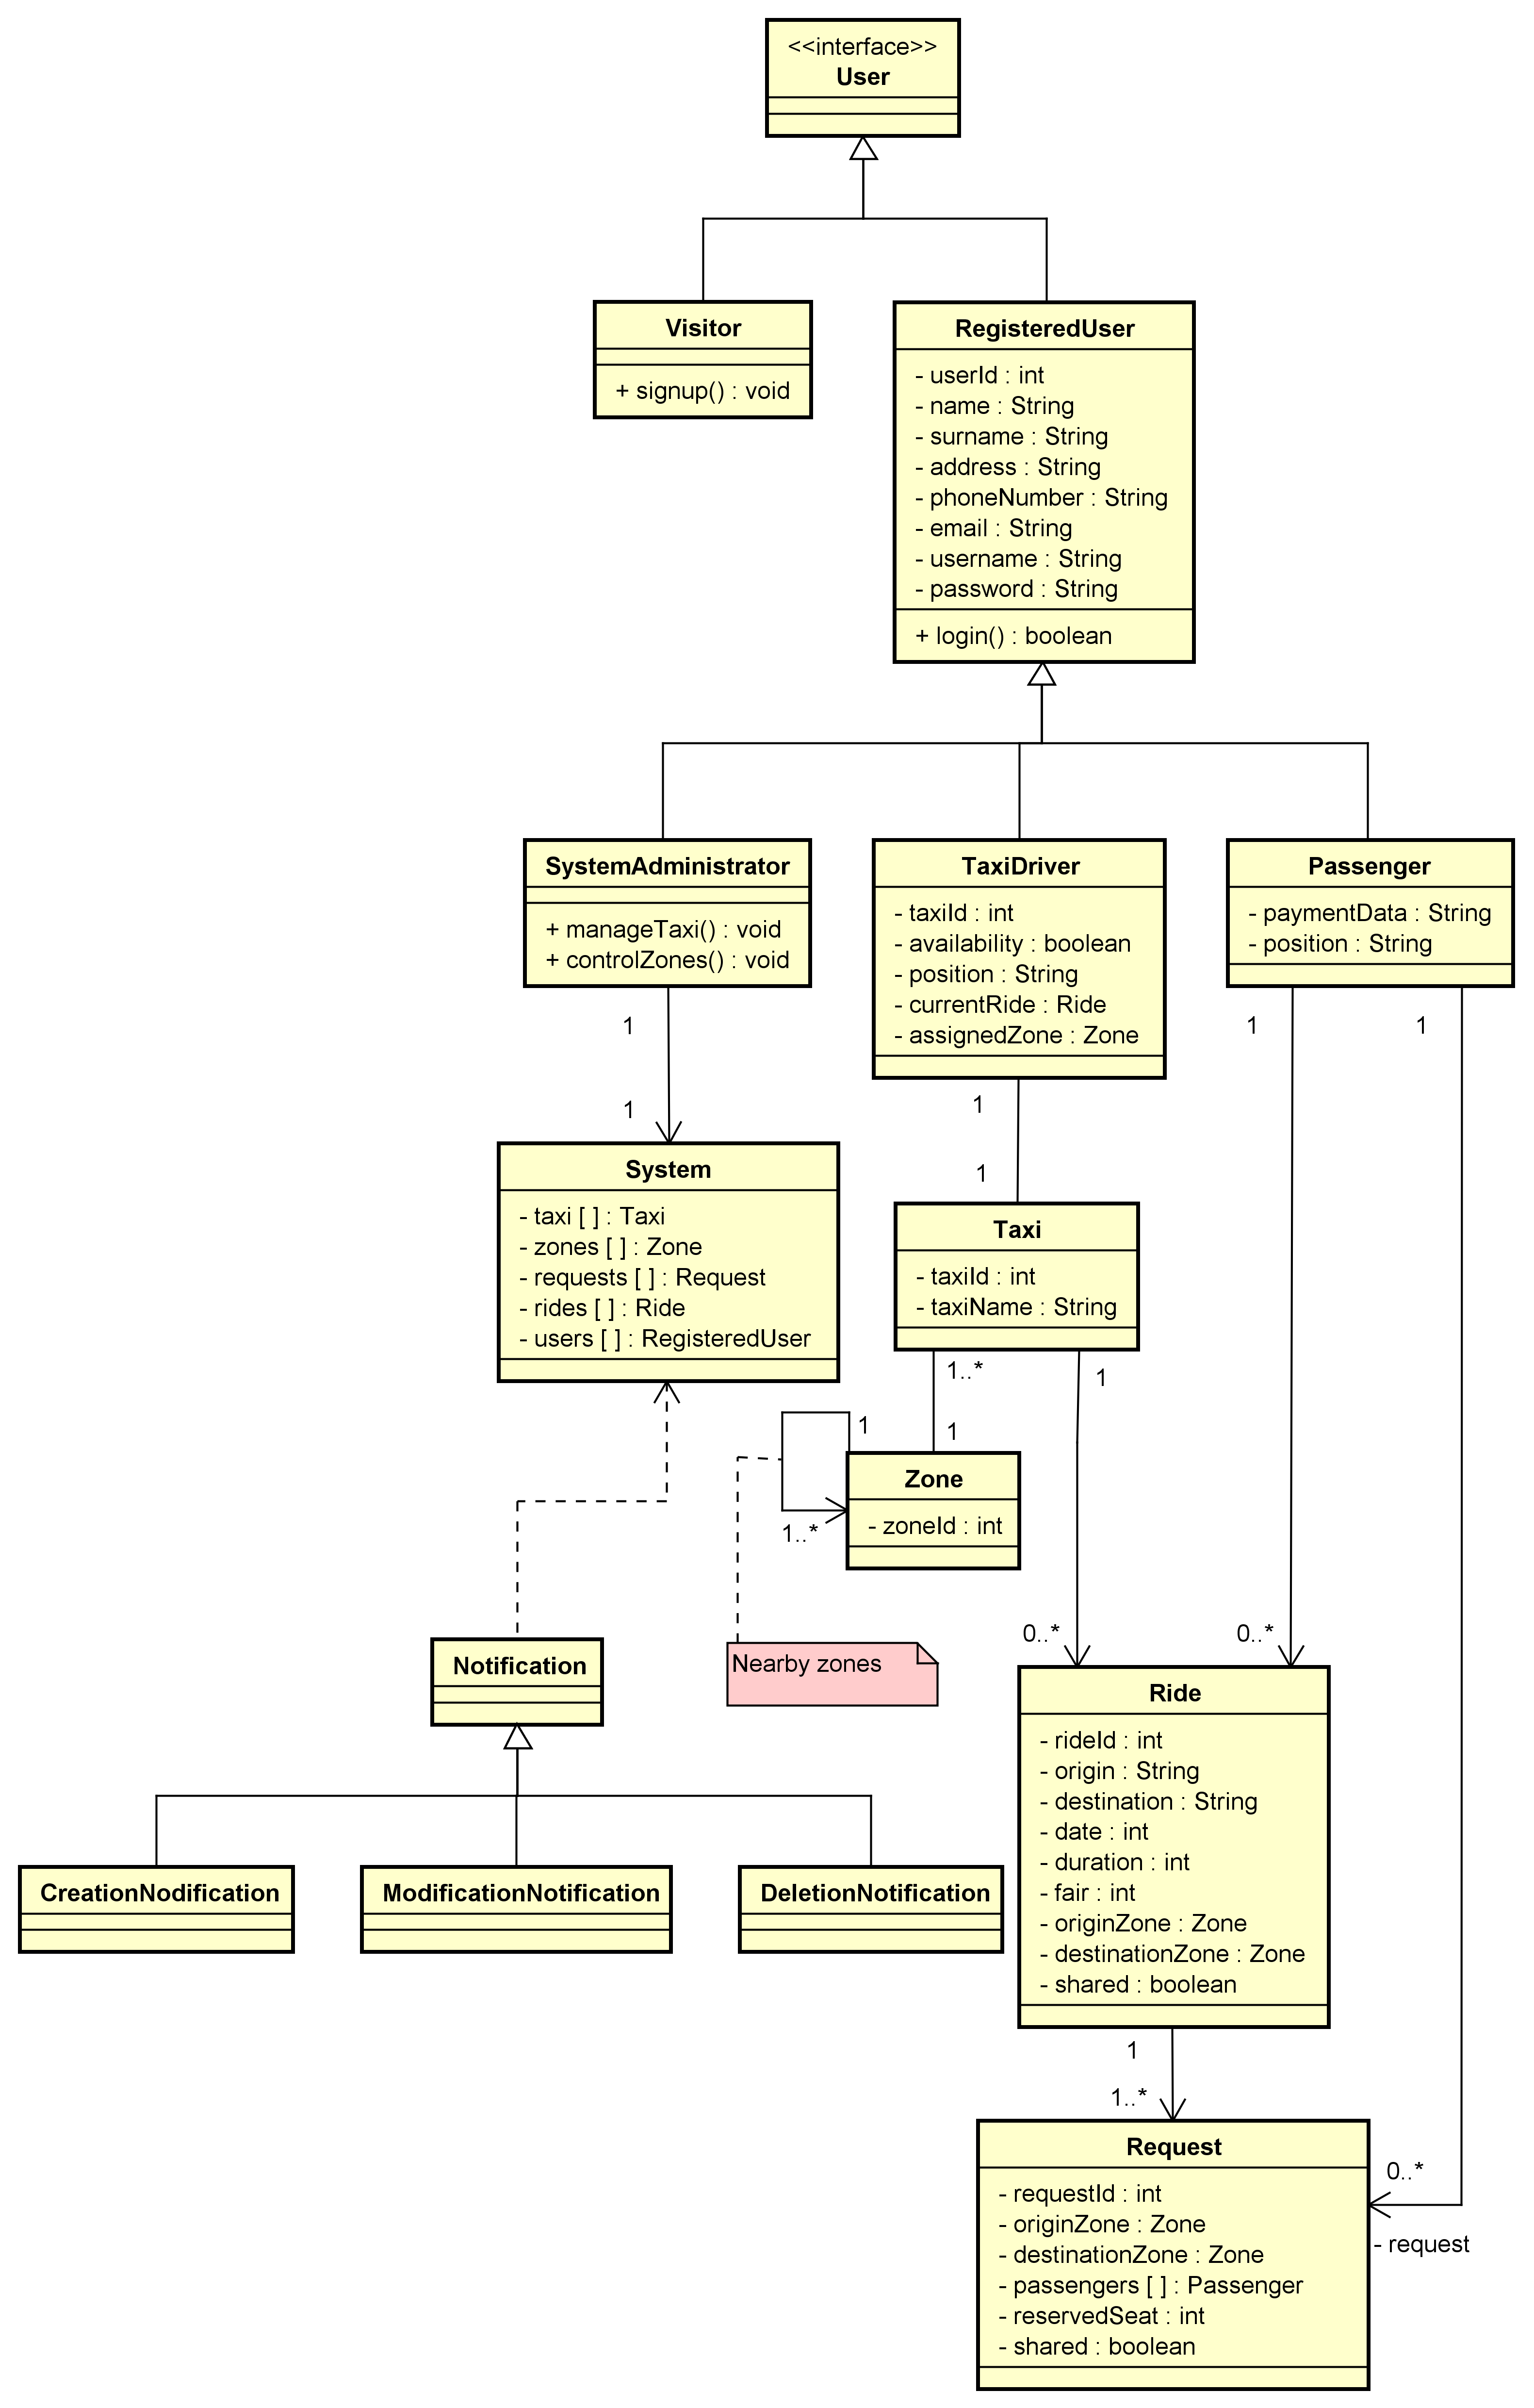
\includegraphics[width=1.4\linewidth]{Pictures/ClassDiagram}}
%			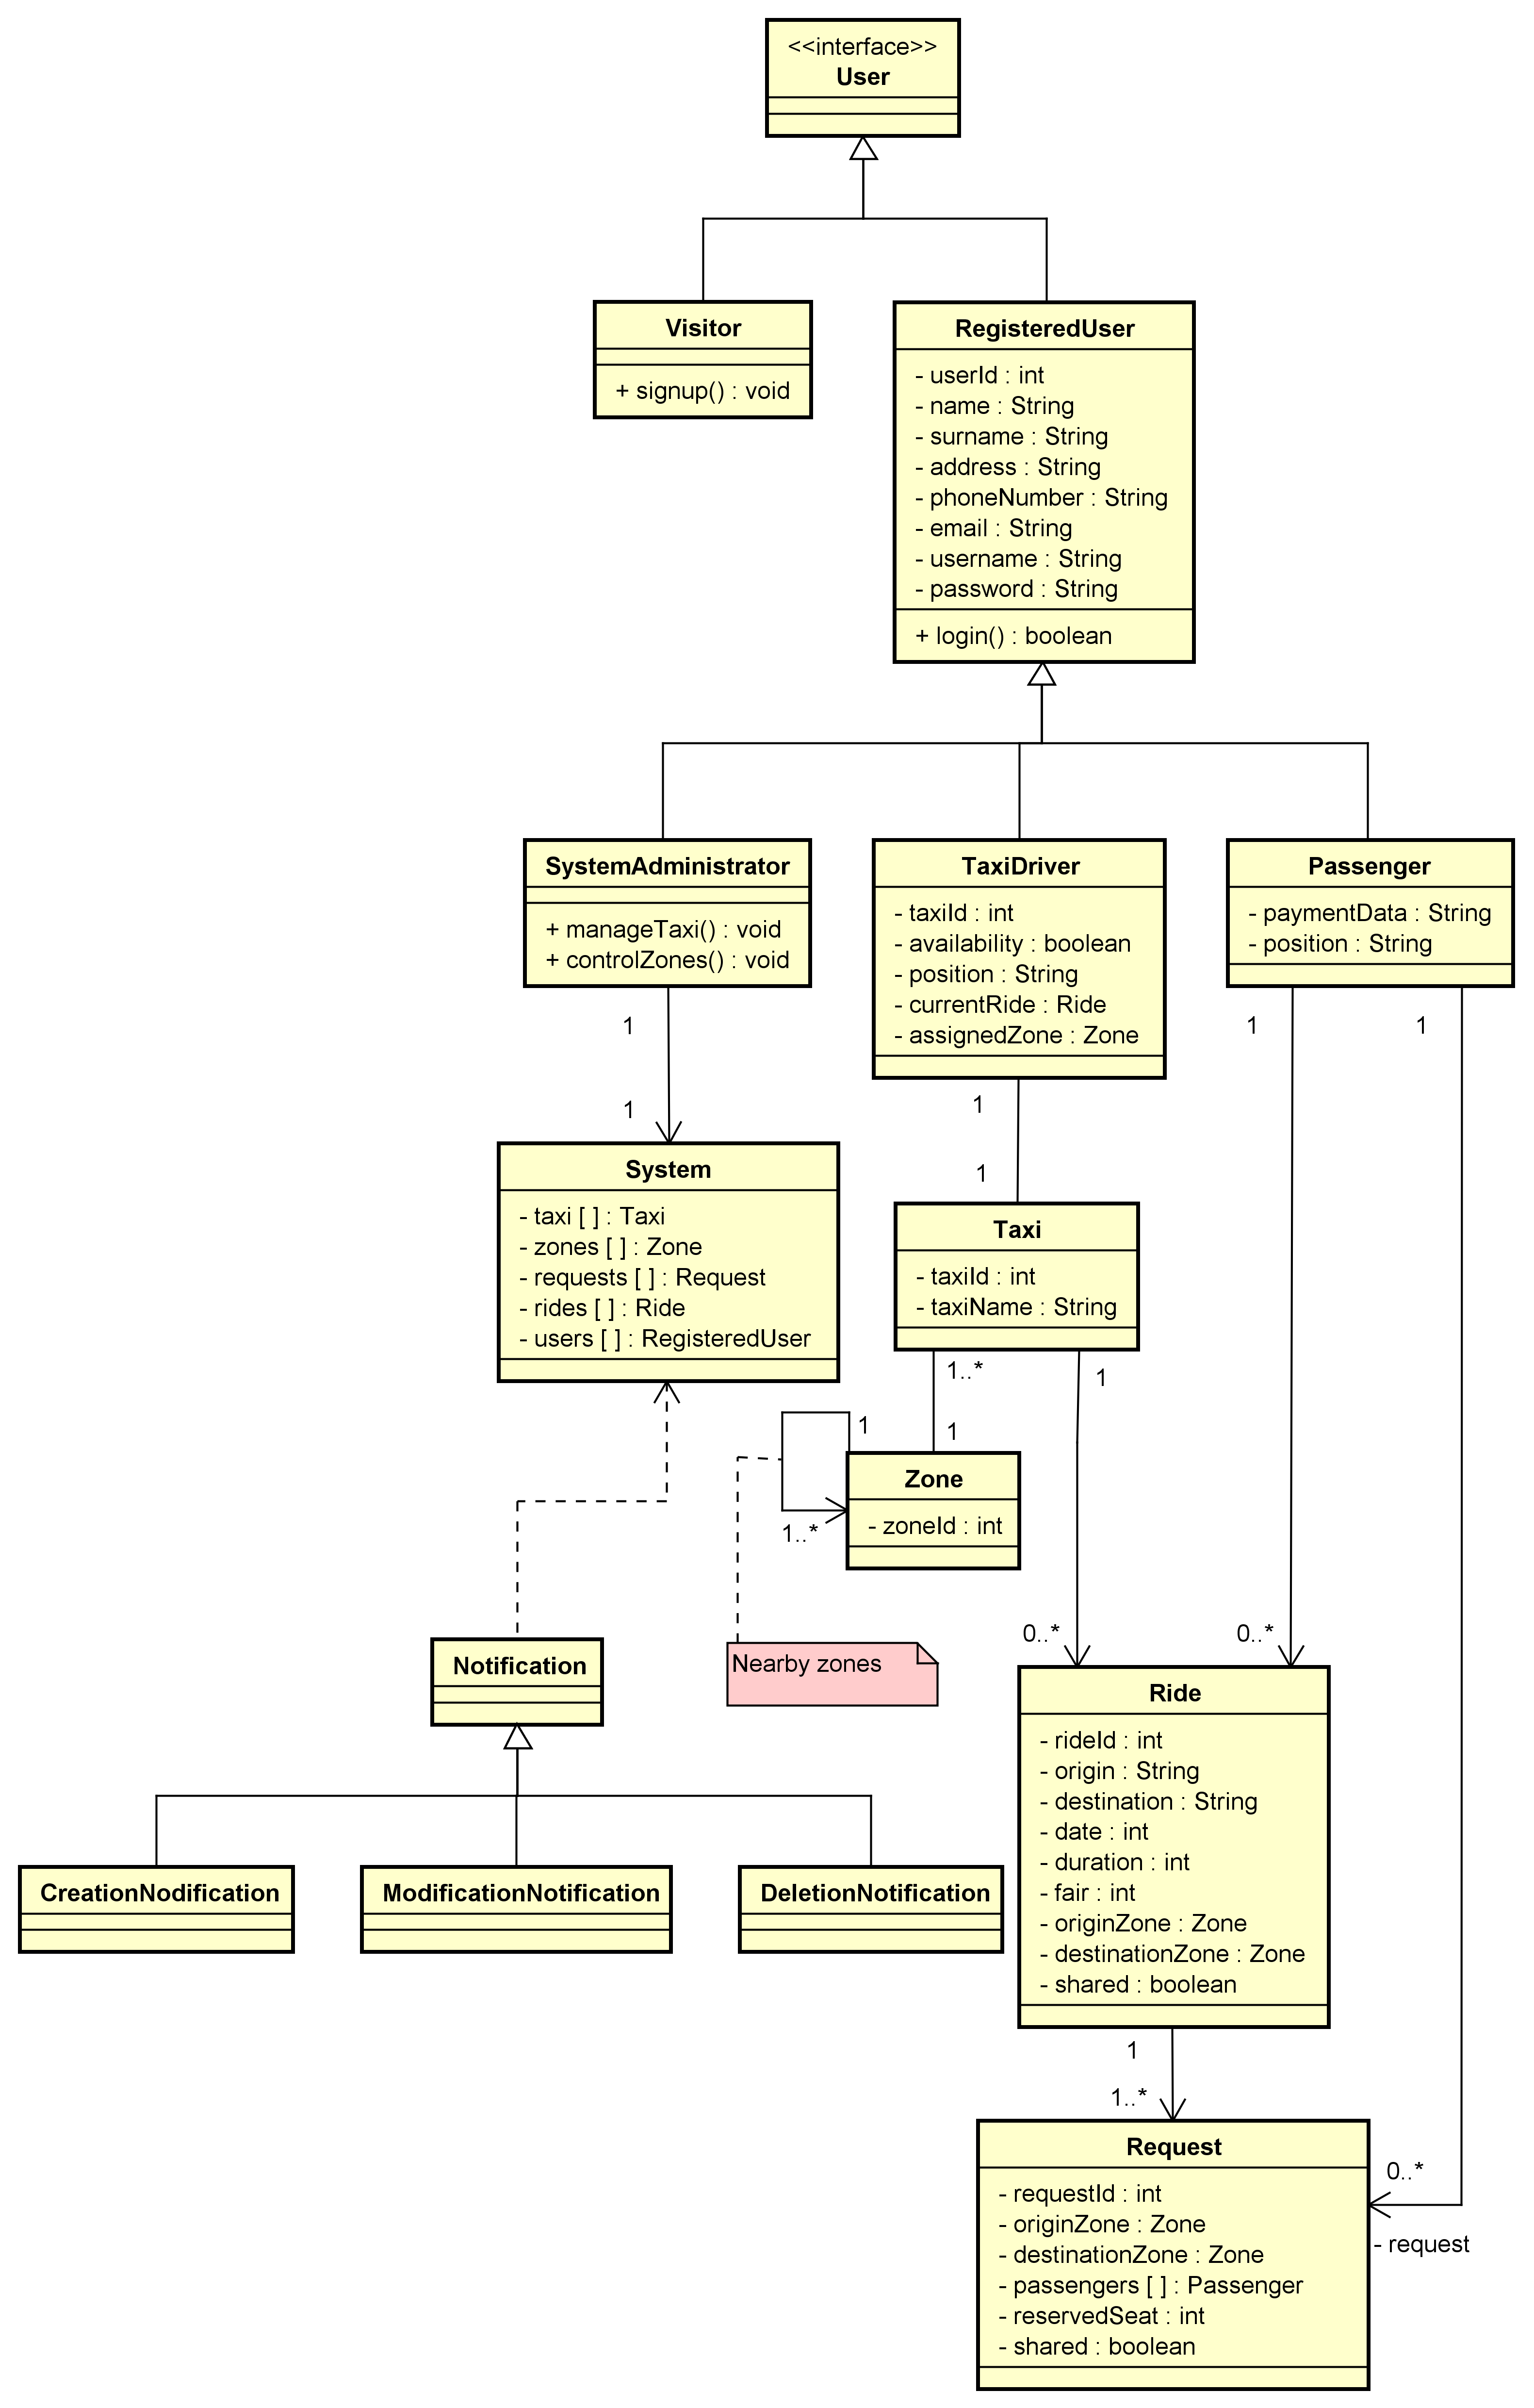
\includegraphics[width=1\linewidth]{Pictures/ClassDiagram}
%		\end{center}
%		\vfill

%	\begin{figure}[p]
%%		\vspace*{-3cm}
%%		\hspace*{-1cm}
%		\centering
%		\makebox[\linewidth]{
%		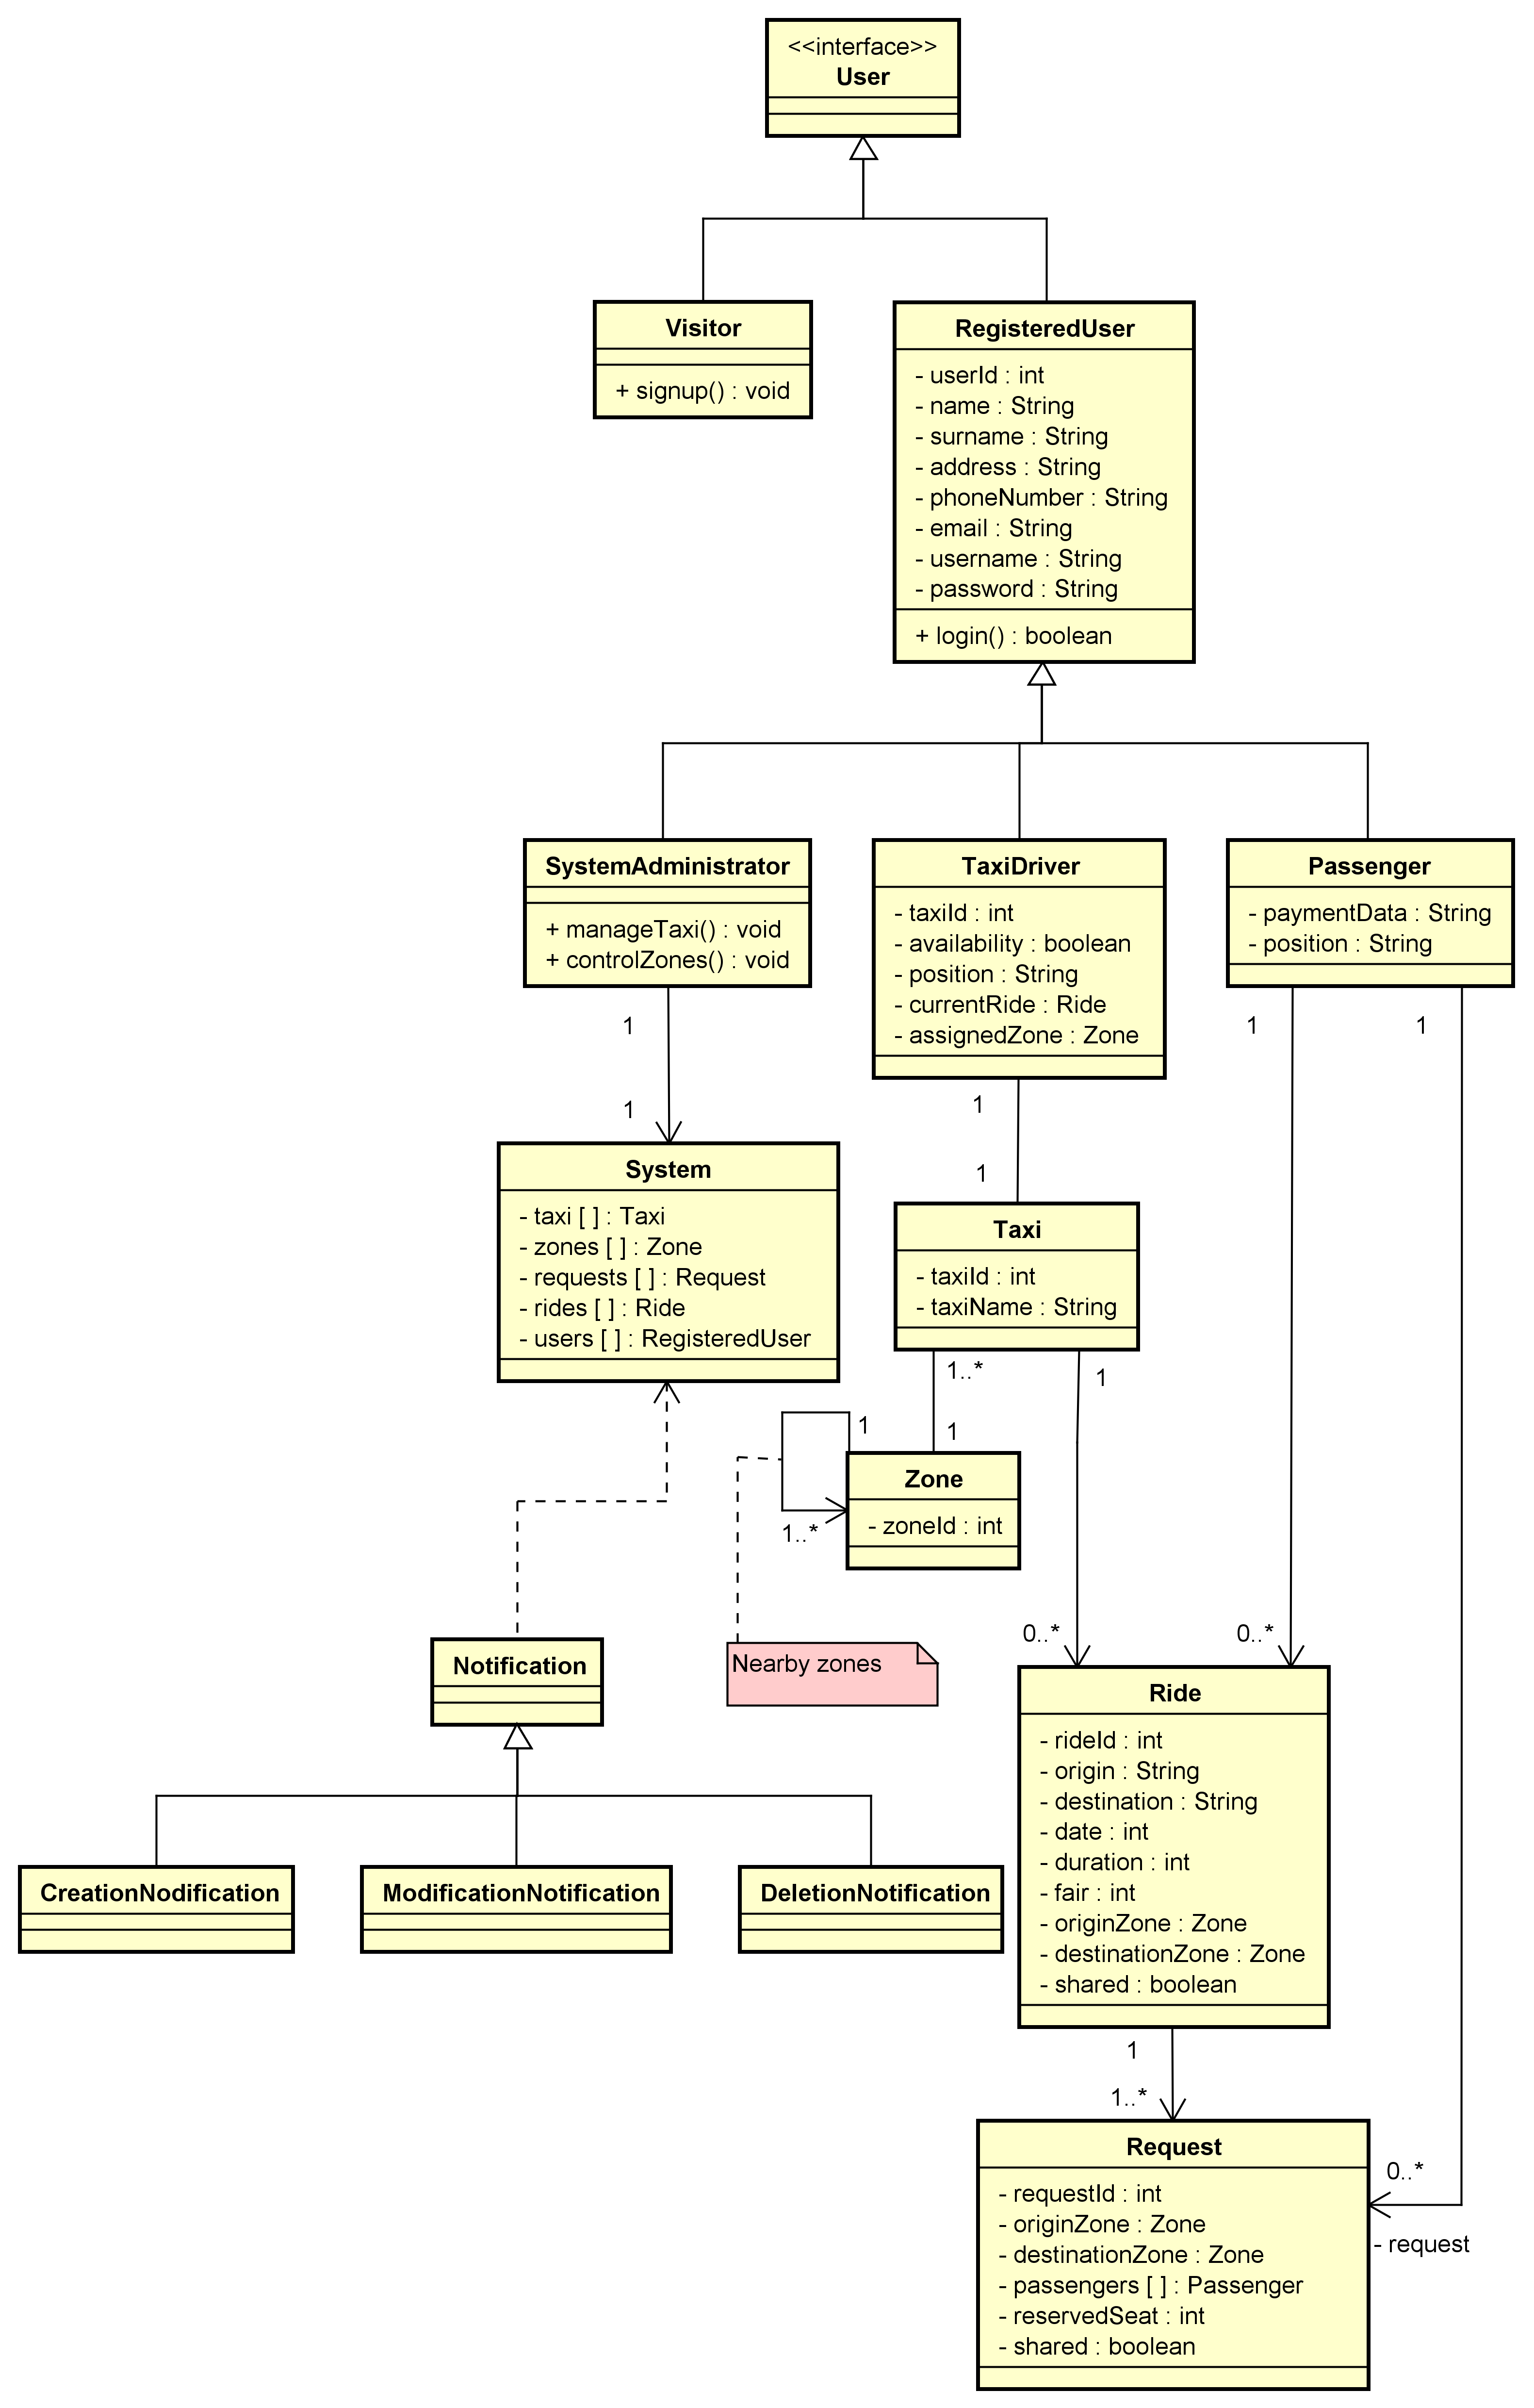
\includegraphics[width=1.3\linewidth]{Pictures/ClassDiagram}
%		}
%	\end{figure}
%	\restoregeometry
	
	
	\pagebreak
	
	\subsubsection{State Machine Diagrams} 
%		\noindent%
%		\begin{minipage}{\linewidth}
%%			\vspace*{-0.35cm}
%			\makebox[\linewidth]{
%				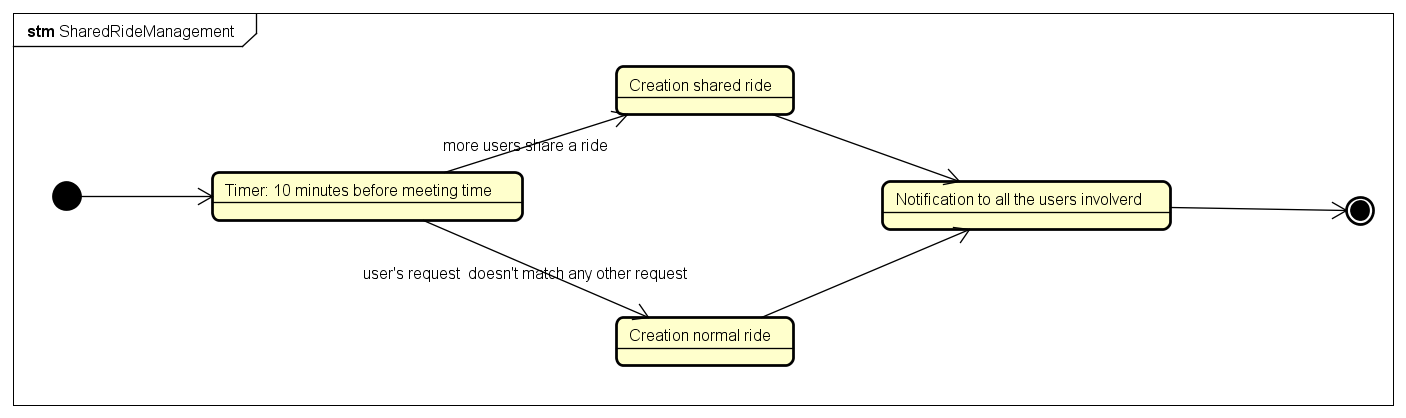
\includegraphics[keepaspectratio=true,scale=0.56]{Pictures/STMSharedRideManagement}}
%		\end{minipage}		
	
	\pagebreak
		
	\subsection{Non Functional Requirements}
	
	\subsubsection{Performance Requirements} The service must guarantee an high level of usability, also in terms of processing and response time of the several functions. The objective is to avoid the situation in which the server represents the bottleneck of the entire system when there are many connections at the same time. To prevent this the server must be correctly chosen and calibrated to handle a large amount of connections in situations of heavy loads. 
	
	\subsubsection{Design Constraints}
		
	\subsubsection{Standards compliance}
	
	\subsubsection{Hardware limitations}
	
	\subsubsection{Software System Attributes}
	
	\paragraph{Availability \& Reliability} \mts{} system must be always accessible. The server that hosts the service is online 24/7 and is equipped with an autonomous power supply backup system.
	
	\paragraph{Security} \mts{} offers a high grade of privacy and security thanks to the protocols that it enforces. As already stated above it requires a 2-factor verification process during the registration; in this way the account is confirmed by two codes that are sent to both the provided email address and phone number. In this way it's verified that  all the means used to communicate with the user really belong to him/her. The application also guarantees an appropriate level of confidentiality and integrity of the sensitive data exchanged on the Web with the server. The DB on the server is behind a DMZ in which is located the web server; firewalls with different rules are used to separate the different ``zones'' of access rights and permissions in the network.
	
	\paragraph{Maintainability} The software itself does not require any particular periodic update, unless the taxi company wants to add some functionalities. The only feature that could require some maintenance are the APIs offered by the system, but again, in this document and all the other ones related to \mts{} that will be attached, future developers can find all what they could need to understand how the system works and then how to update some sections of the software. 

	\paragraph{Portability}
	
	\subsection{Other Requirements}
	
	\pagebreak

	\section{Alloy}
	\lstinputlisting[language=alloy,basicstyle=\normalsize]{Alloy/myTaxyService.als}
	
	\pagebreak
	
	\section{Appendix}
	
	\subsection{Software and tools used}
	\begin{itemize}
		\item TeXstudio 2.10.4 (http://www.texstudio.org/) to redact and format this document.
		\item Astah Professional 7.0 (http://astah.net/editions/professional): to create Use
		Cases Diagrams, Sequence Diagrams, Class Diagrams and State Machine	Diagrams.
		\item Alloy Analyzer 4.2 (http://alloy.mit.edu/alloy/) to prove the consistency of
		the model.
		\item Balsamiq Mockups 3.2.4 (http://balsamiq.com/products/mockups/) to create the mockups.
	\end{itemize}
	
	\subsection{Hours of work} The time spent to redact this document:
	\begin{itemize}
		\item Baldassari Alessandro: xx hours.
		\item Bendin Alberto: xx hours.
		\item Giarola Francesco: xx hours.
	\end{itemize}
	
	
\end{document}